\subsection{Implementation Details}
\begin{itemize}
  \item Number of bins used, depth range, laser parameters, use of intensity
    image.
  \item Using
\end{itemize}
\paragraph{NYU Depth v2}
The NYU Depth v2 Dataset consists of 249 training and 215 testing scenes of
RGB-D data captured using a Microsoft Kinect. We used a version of DORN
<<<<<<< HEAD
pretrained according to \cite{Fu. et al} as our CNN.
=======
pretrained according to \cite{Fu2018} as our CNN.
>>>>>>> ac23c73116b7fdd108ca4951a414a00ea9b25df3
\newpage
% \begin{table*}
% \begin{center}
% \begin{tabular}{lccc|ccc}
%   \toprule
%     & $\delta^1 \uparrow$ & $\delta^2\uparrow$ & $\delta^3 \uparrow$ & RMSE $\downarrow$ & rel $\downarrow$ & $log_{10} \downarrow$ \\
%   \midrule
% Eigen et. al. & 0.769 & 0.950 & 0.988 & 0.641 & 0.158 & - \\ 
% Laina et. al.&0.811&0.953&0.988&0.573&0.127&0.055 \\
% DORN&0.818&0.950&0.982&0.620&0.137&0.063 \\
%   DORN (rescaled) & 0.872 & 0.967 & 0.989 & 0.548 & 0.111 & 0.048 \\
% Alhashim, Wonka (2019)&0.847&0.973&0.994&0.548(0.461)&0.123&0.053 \\
% Alhashim, Wonka (2019) rescaled using GT depth"&0.888&\textbf{0.978}&\textbf{0.995}&\textbf{0.499}(0.409)&\textbf{0.106}&\textbf{0.045} \\
%   \midrule
%   Ours (raw depth counts) & \textbf{0.899} & 0.970 & 0.990 & 0.529 & 0.199 & 0.055 \\
%   Ours (DORN) (intensity/falloff) & 0.835 & 0.953 & 0.984 & 0.521 & 0.129 & 0.060 \\
%   Ours (DenseDepth) (intensity/falloff) & 0.867 & 0.974 & 0.994 & 0.445 & 0.114 & 0.050 \\
%   \bottomrule
% \end{tabular} 
% \end{center}
% \caption{Results on the NYU Depth v2 test set \cite{nyudepth}.}
% \end{table*}
%%%
\begin{table*}
\begin{center}
\begin{tabular}{llrrr|rrr}
\toprule
           &                & $\delta1 \uparrow$ & $\delta2 \uparrow$ & $\delta3 \uparrow$ & $rel \downarrow$ & $rmse \downarrow$ & $log10 \downarrow$ \\
model & hyperparams &                    &                    &                    &                  &                   &                    \\
\midrule
\multirow{6}{*}{dorn} & CNN &              0.846 &              0.954 &              0.983 &            0.120 &             0.501 &              0.053 \\
           & CNN + median rescaling &              0.871 &              0.964 &              0.988 &            0.111 &             0.473 &              0.048 \\
           & CNN + GT histogram matching &              0.906 &              0.972 &              0.990 &            0.095 &             0.419 &              0.040 \\
           & Ours (SBR=10) &              0.903 &              0.970 &              0.989 &            0.091 &             0.422 &              0.040 \\
           & Ours (SBR=50) &              0.906 &              0.971 &              0.990 &            0.089 &             0.410 &              0.039 \\
           & Ours (SBR=100) &              0.906 &              0.971 &              0.990 &            0.090 &             0.408 &              0.039 \\
\cline{1-8}
\multirow{6}{*}{densedepth} & CNN &              0.847 &              0.973 &              0.994 &            0.123 &             0.461 &              0.053 \\
           & CNN + median rescaling &              0.888 &              0.978 &              0.995 &            0.106 &             0.409 &              0.045 \\
           & CNN + GT histogram matching &              0.930 &              0.984 &              0.995 &            0.079 &             0.338 &              0.034 \\
           & Ours (SBR=10) &              0.922 &              0.982 &              0.994 &            0.082 &             0.361 &              0.036 \\
           & Ours (SBR=50) &              0.925 &              0.983 &              0.995 &            0.081 &             0.348 &              0.035 \\
           & Ours (SBR=100) &              0.926 &              0.983 &              0.995 &            0.081 &             0.346 &              0.035 \\
\bottomrule
\end{tabular}

\caption{Simulated Results on NYU Depth v2. Bold indicates best performance for
<<<<<<< HEAD
  that metric, while underline indicates second best.}
\end{center}
\end{table*}

=======
  that metric, while underline indicates second best. The proposed scheme
  outperforms DenseDepth and DORN on all metrics, and even outperforms the
  median rescaling scheme, which has access to the true median depth value.}
\end{center}
\end{table*}


\begin{figure*}
  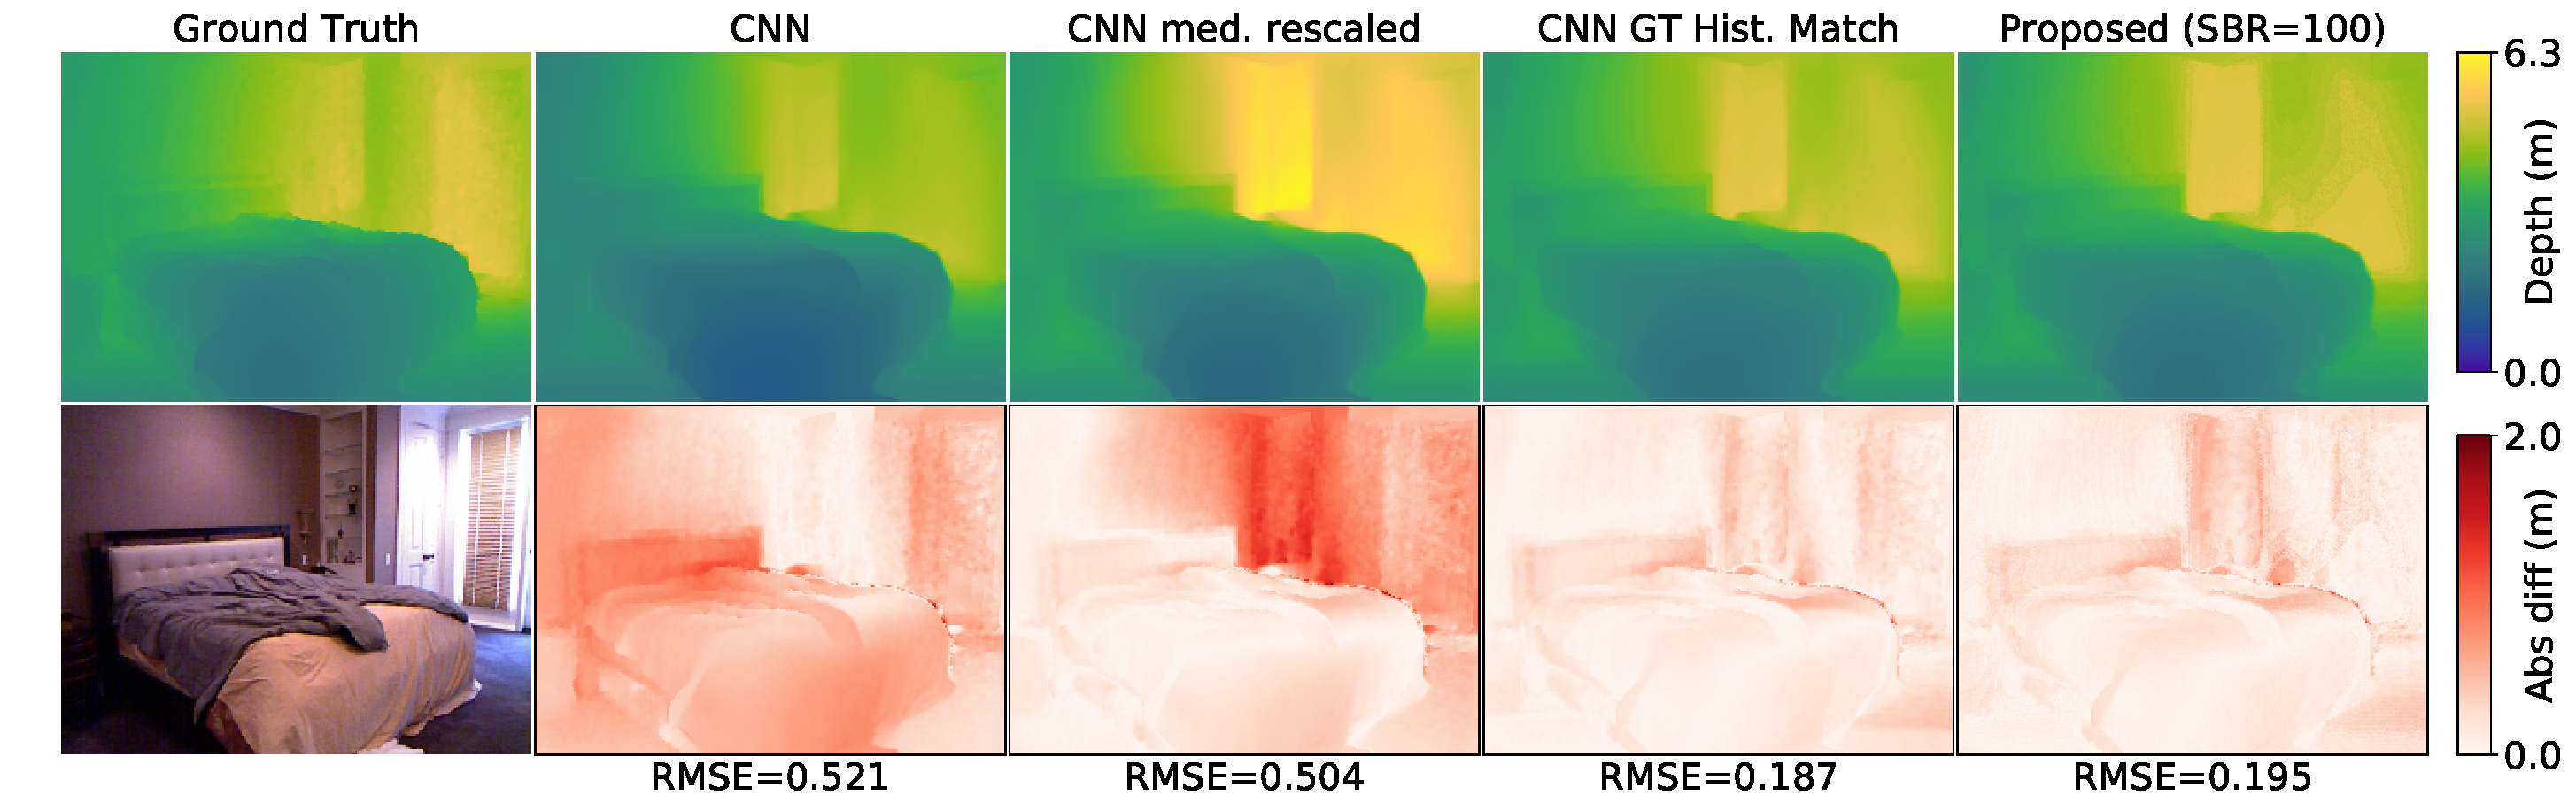
\includegraphics[width=\textwidth]{sections/figures/comparison/densedepth_468_comparison.png}
  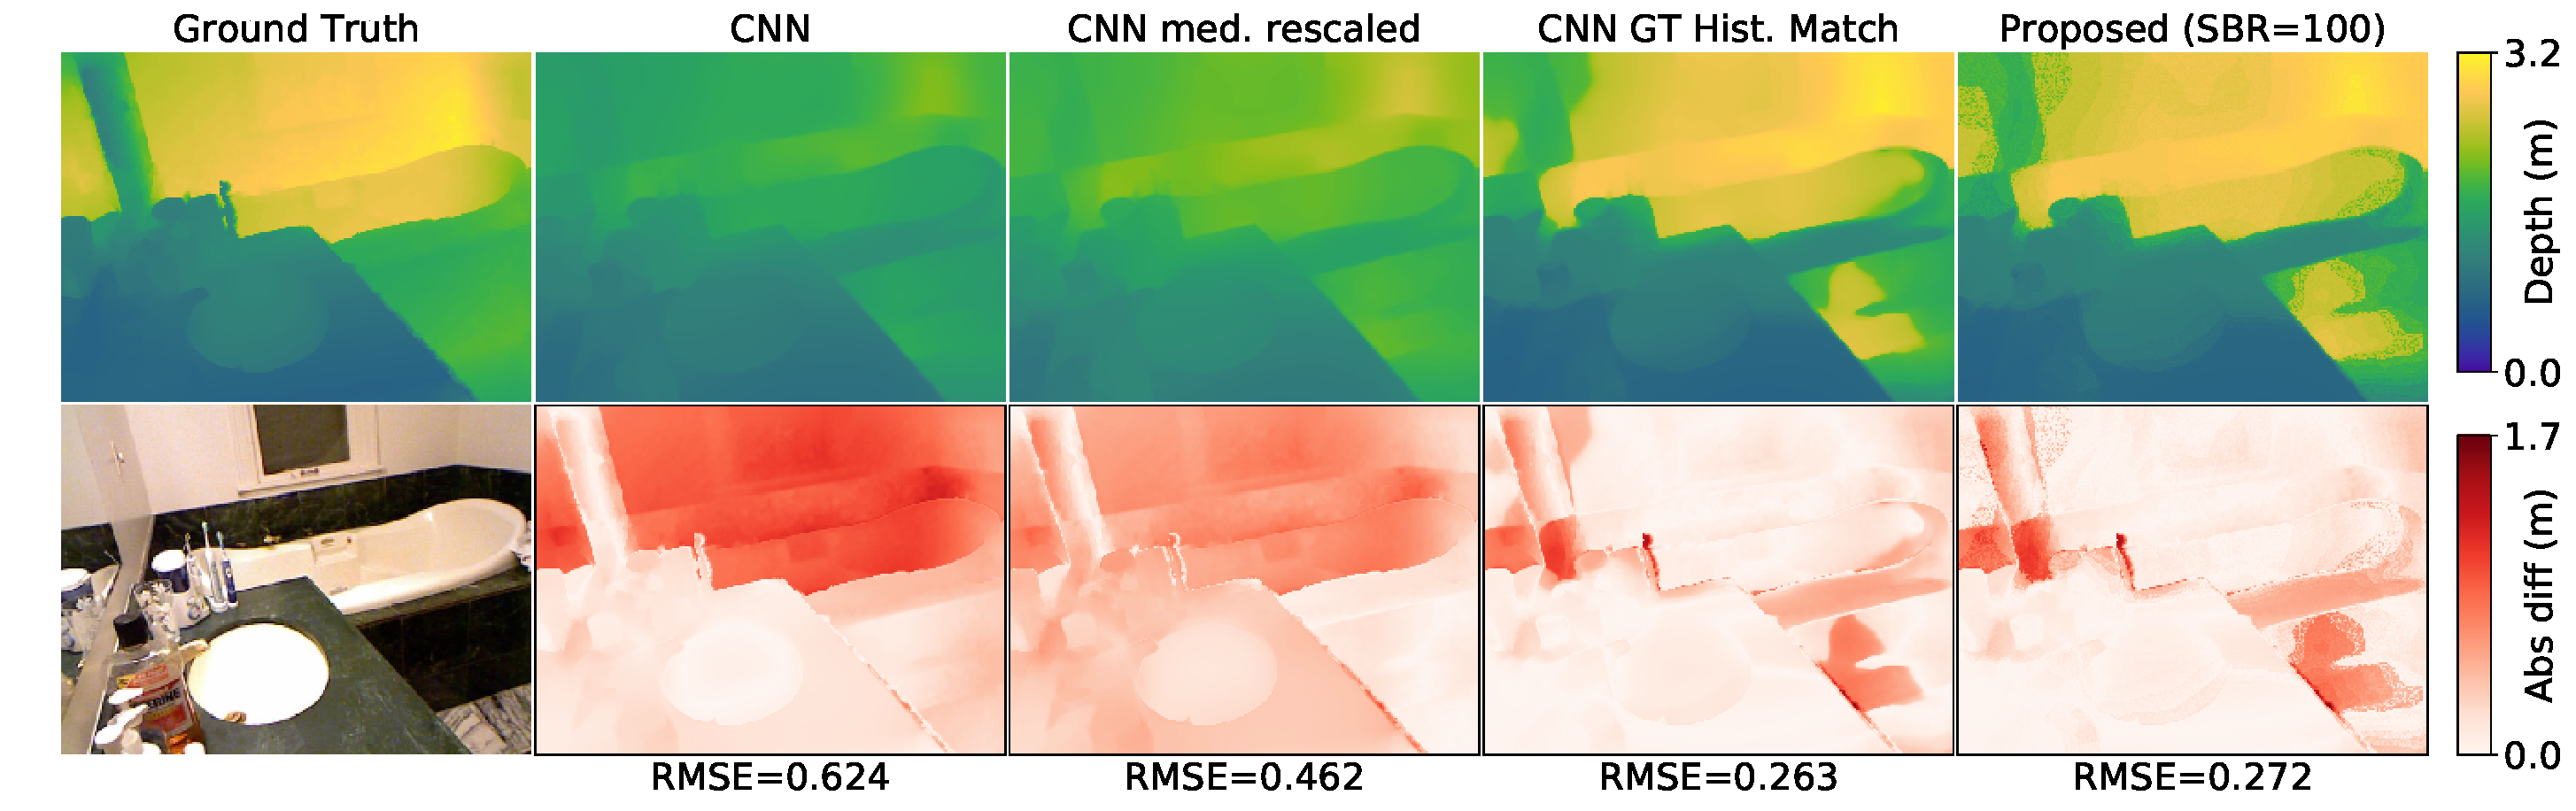
\includegraphics[width=\textwidth]{sections/figures/comparison/densedepth_194_comparison.png}
  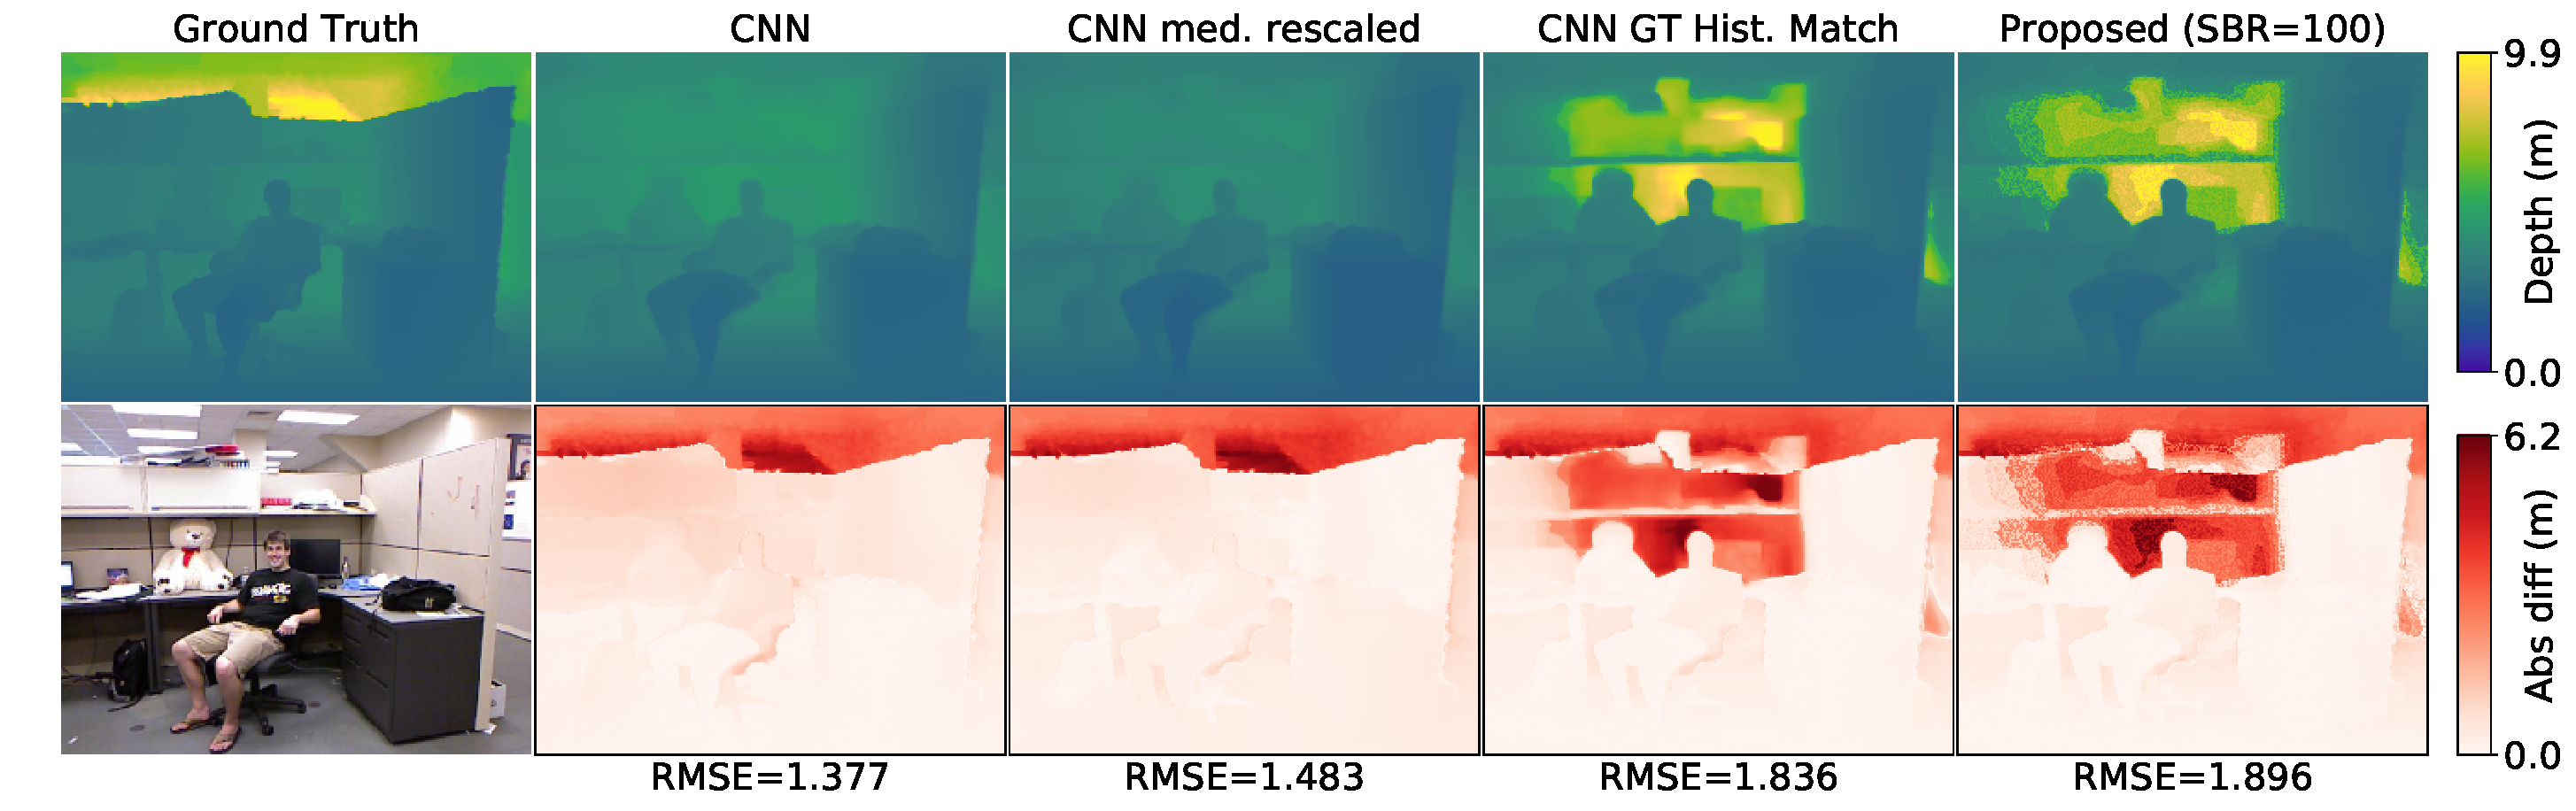
\includegraphics[width=\textwidth]{sections/figures/comparison/densedepth_258_comparison.png}
  \caption{Selected Results on DenseDepth. First two examples demonstrate
    capability of proposed method to correct initial scaling/translation errors.
    Last example shows potential pitfall when ordinal depth is predicted incorrectly.}
\end{figure*}

>>>>>>> ac23c73116b7fdd108ca4951a414a00ea9b25df3
\begin{figure*}
  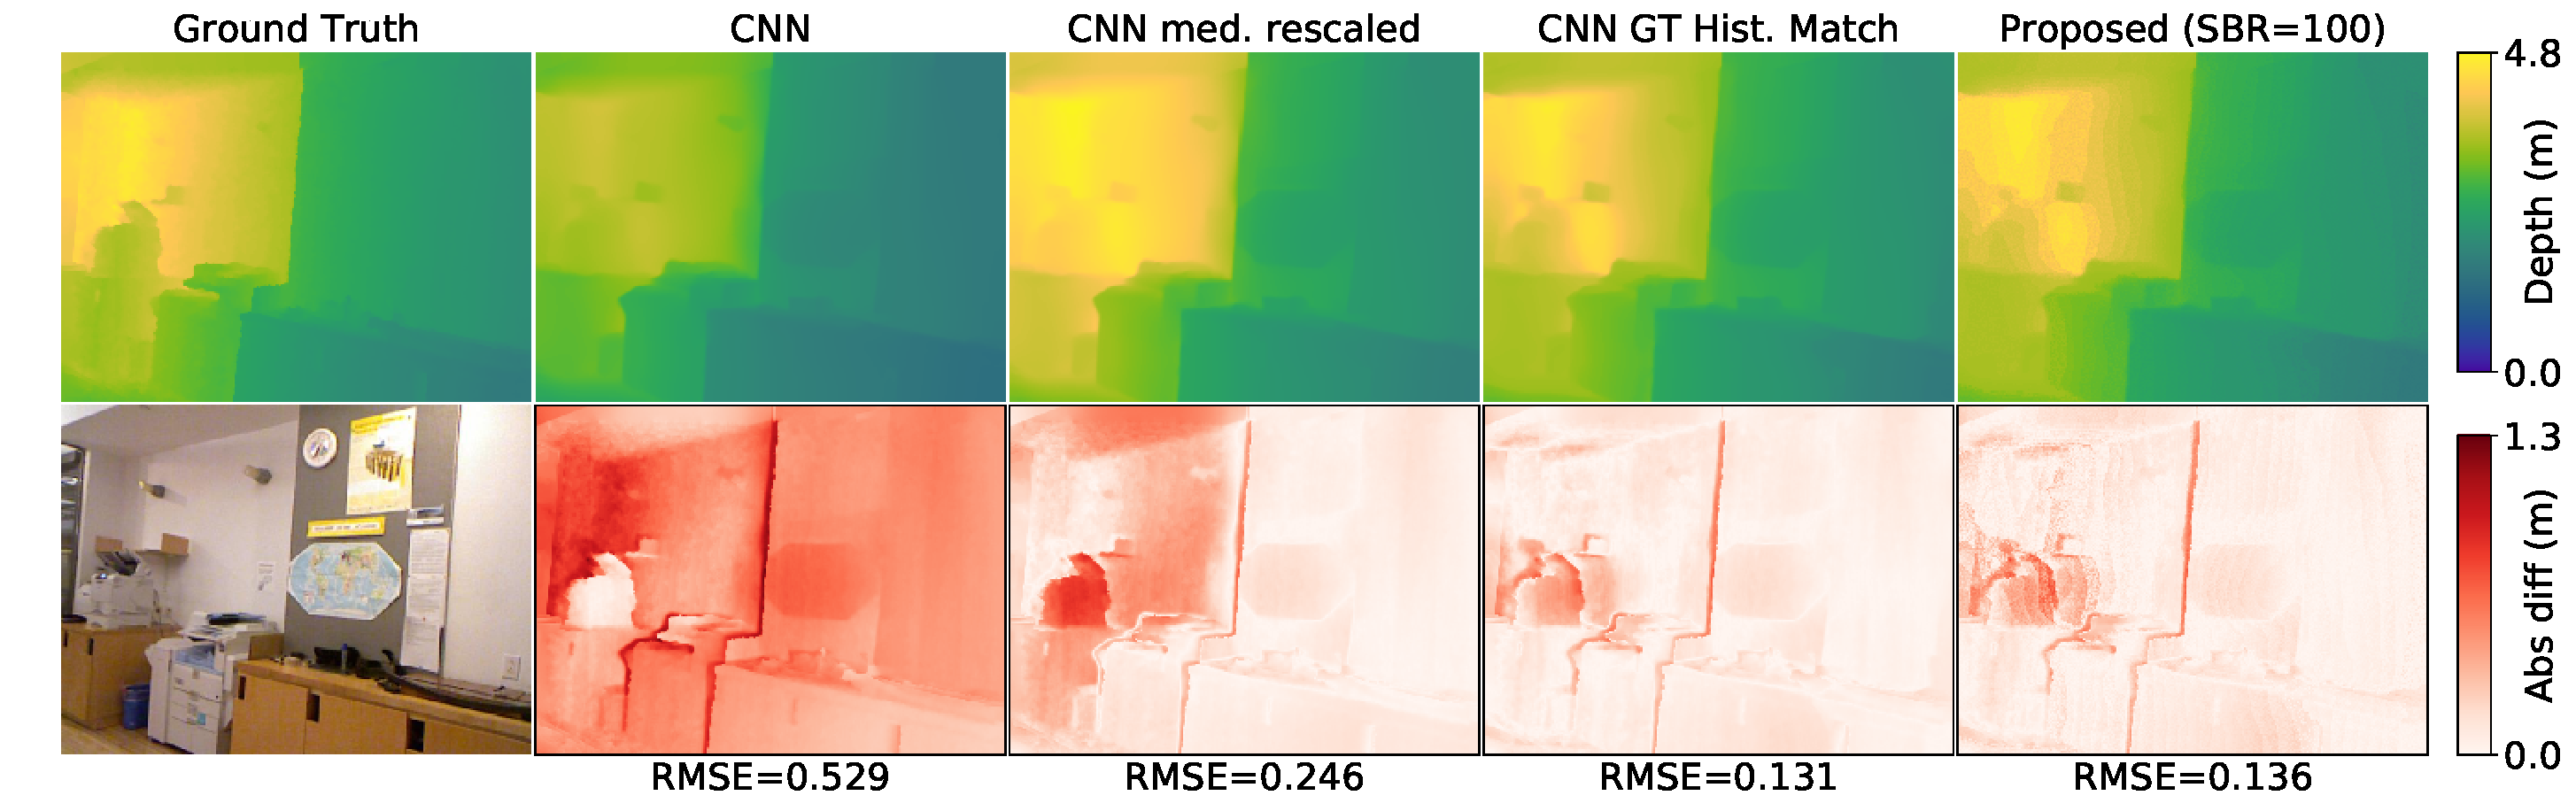
\includegraphics[width=\textwidth]{sections/figures/comparison/densedepth_18_comparison.png}
  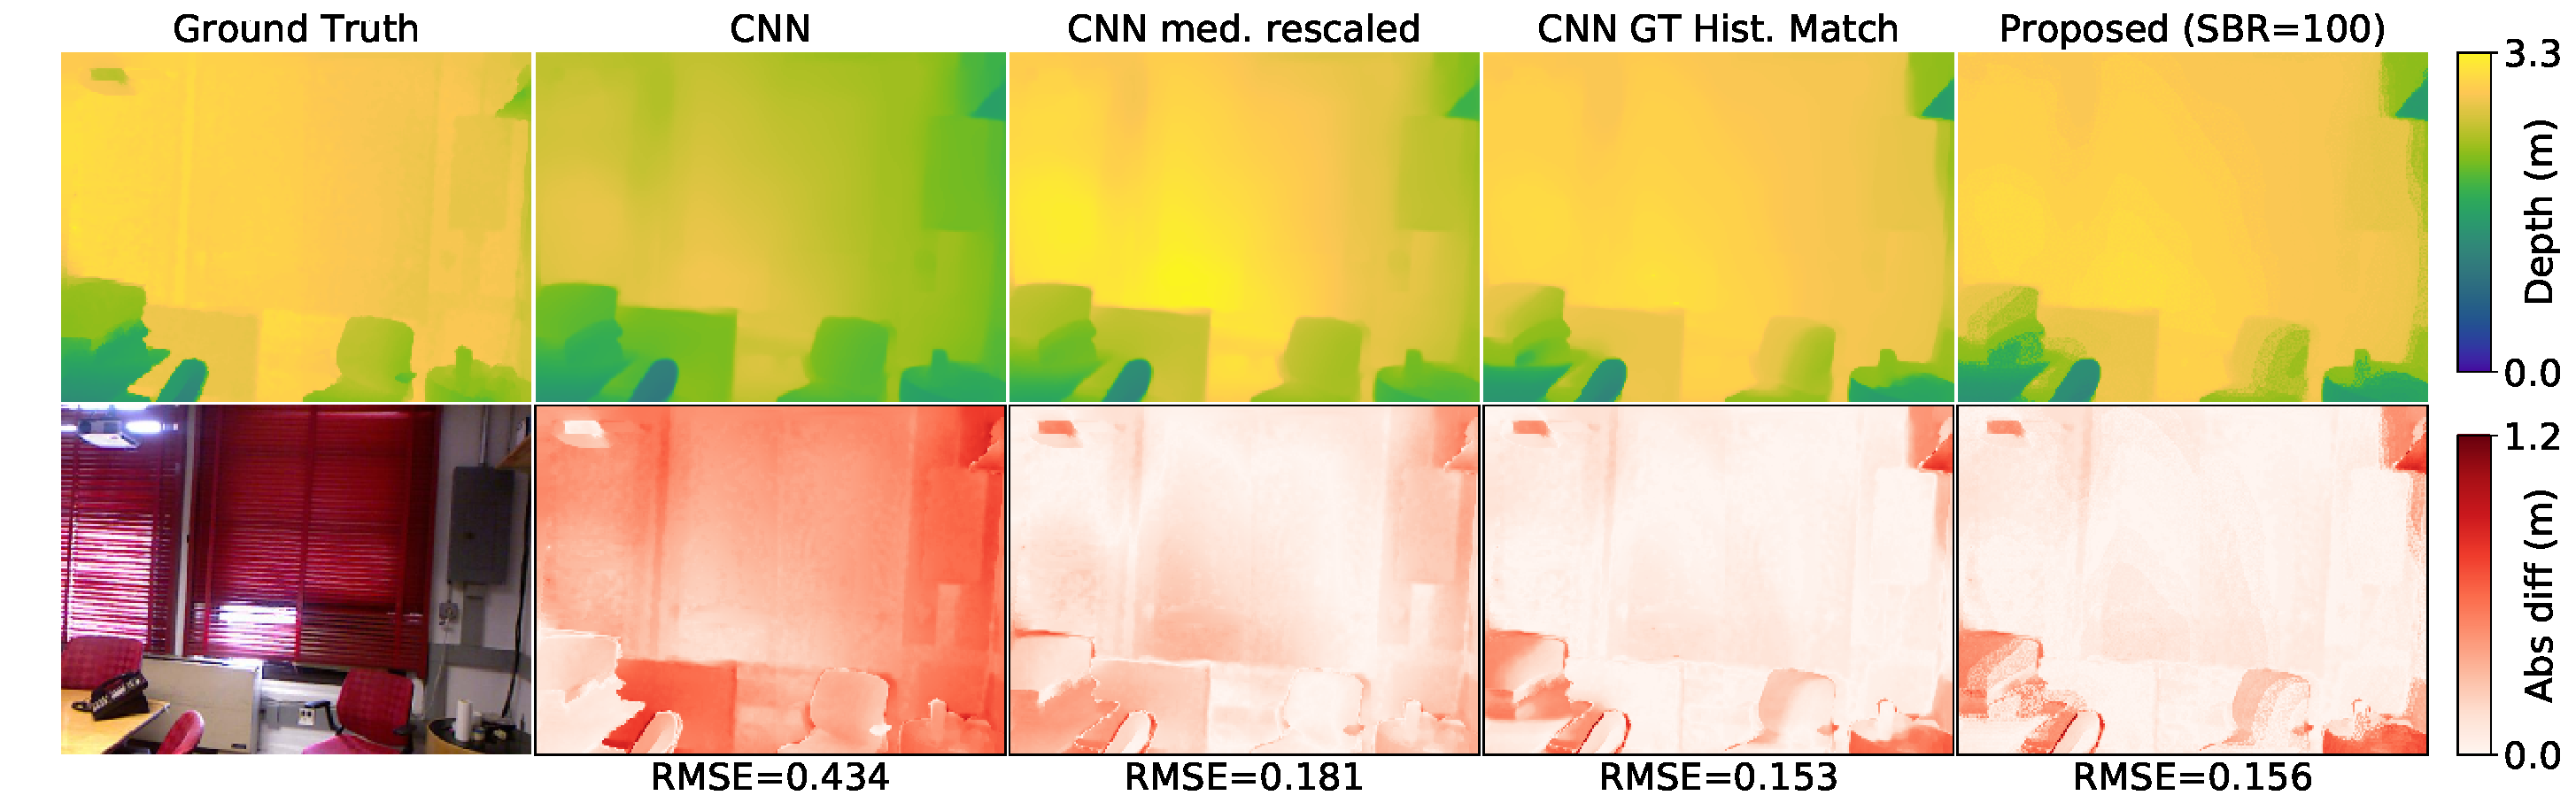
\includegraphics[width=\textwidth]{sections/figures/comparison/densedepth_21_comparison.png}
  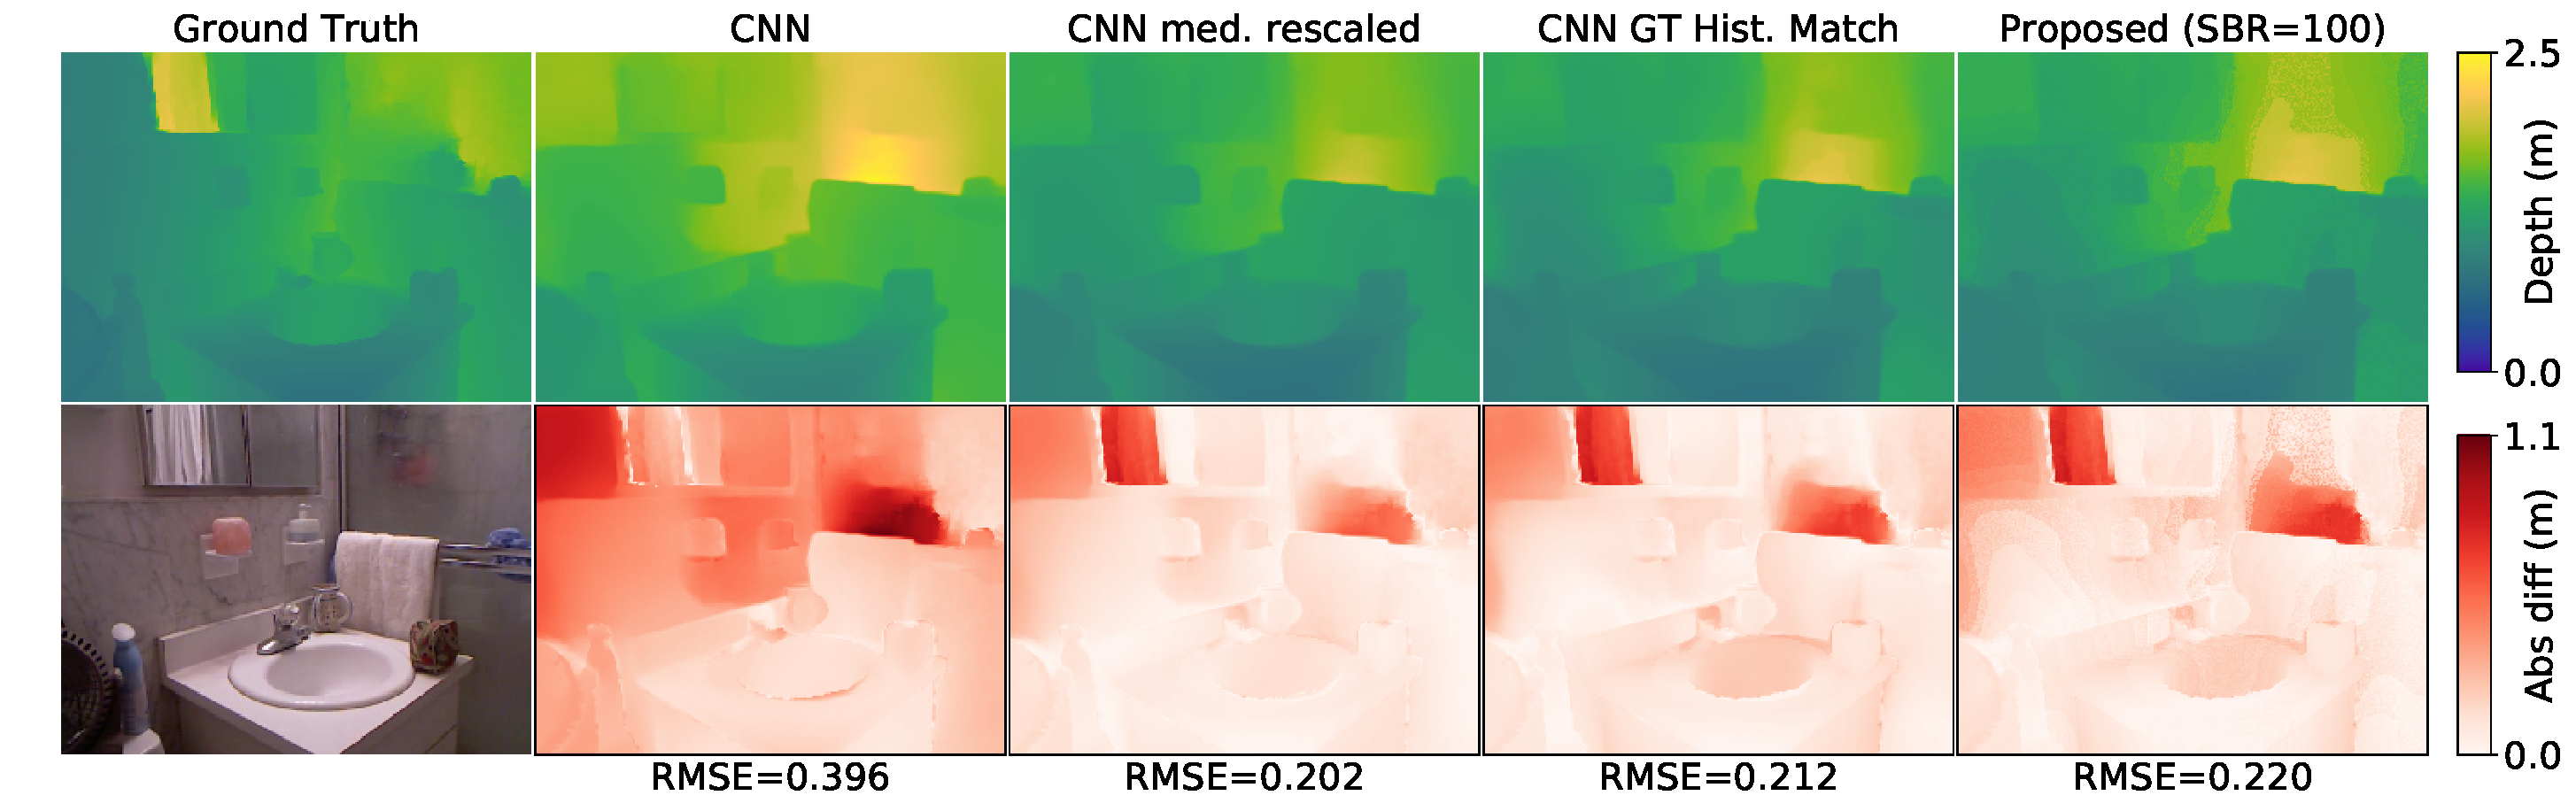
\includegraphics[width=\textwidth]{sections/figures/comparison/densedepth_25_comparison.png}
  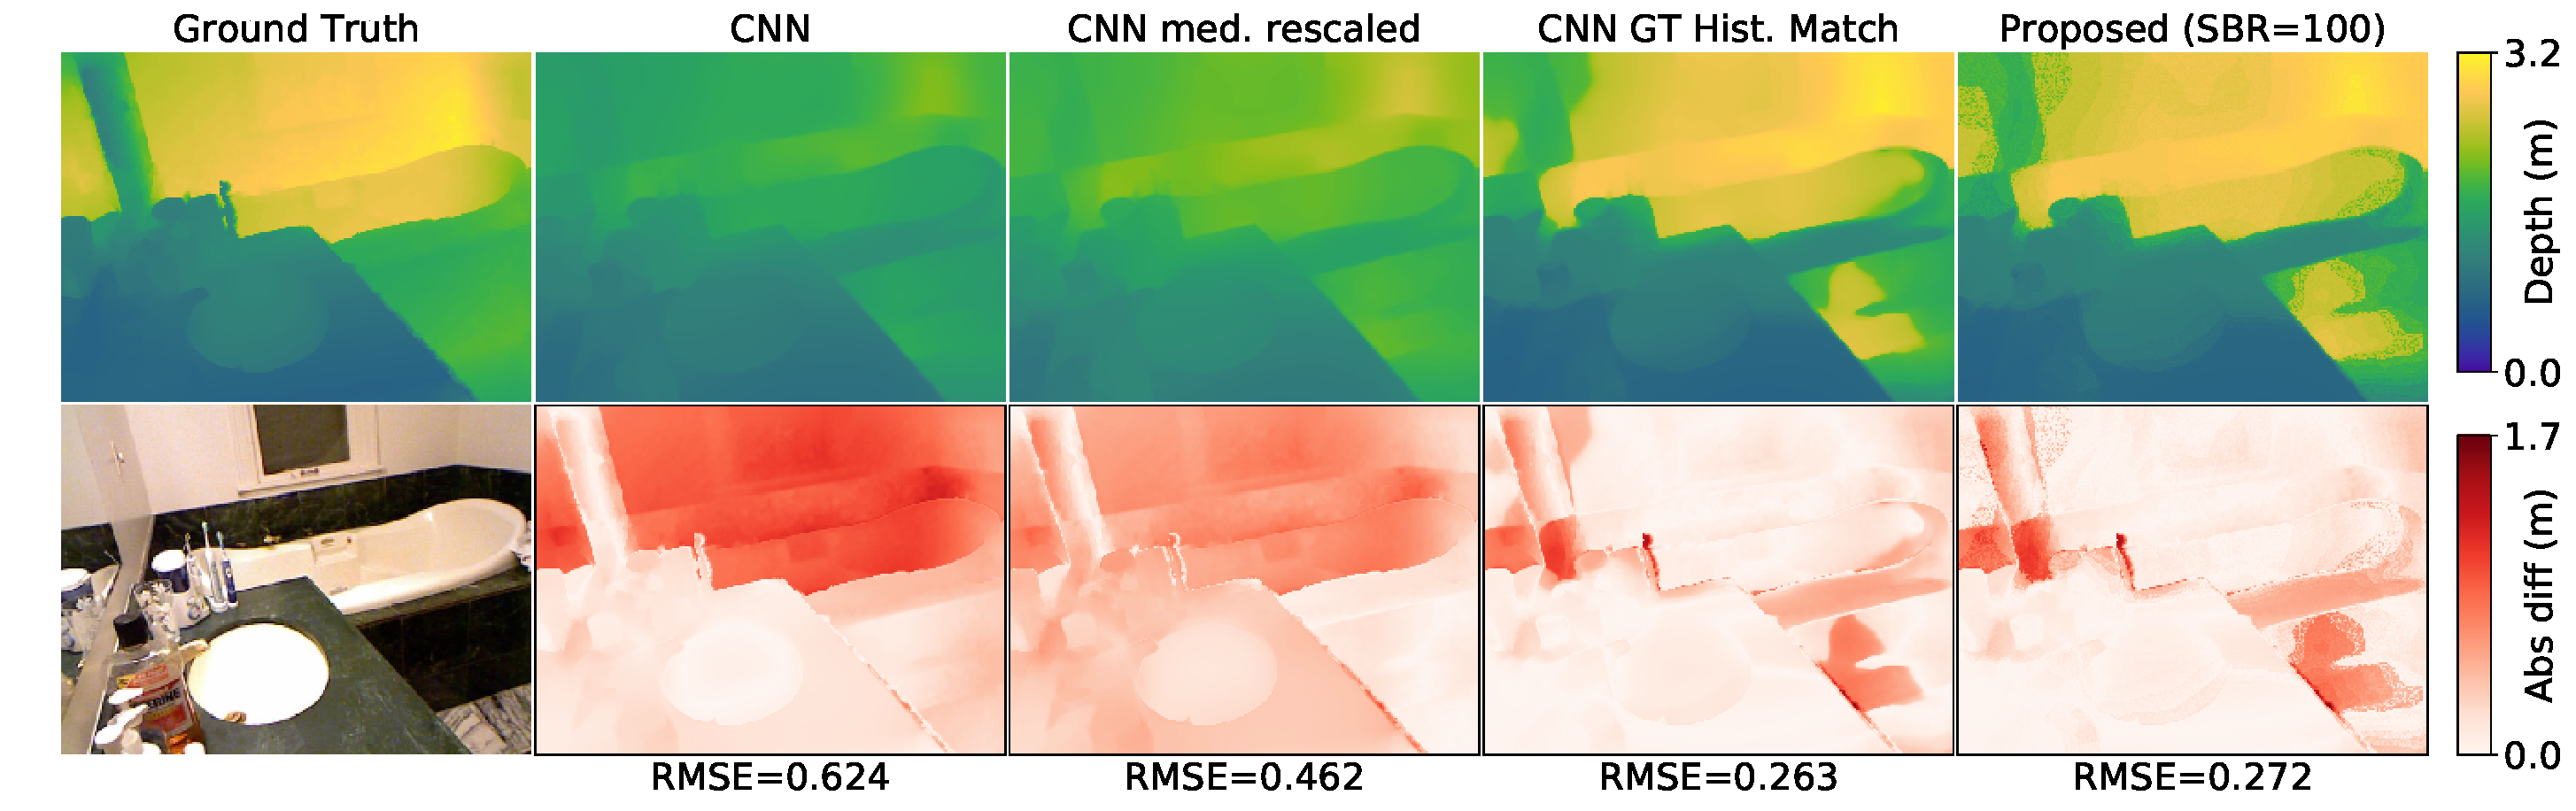
\includegraphics[width=\textwidth]{sections/figures/comparison/densedepth_194_comparison.png}
  \caption{Results on DenseDepth}
\end{figure*}
\begin{figure*}
  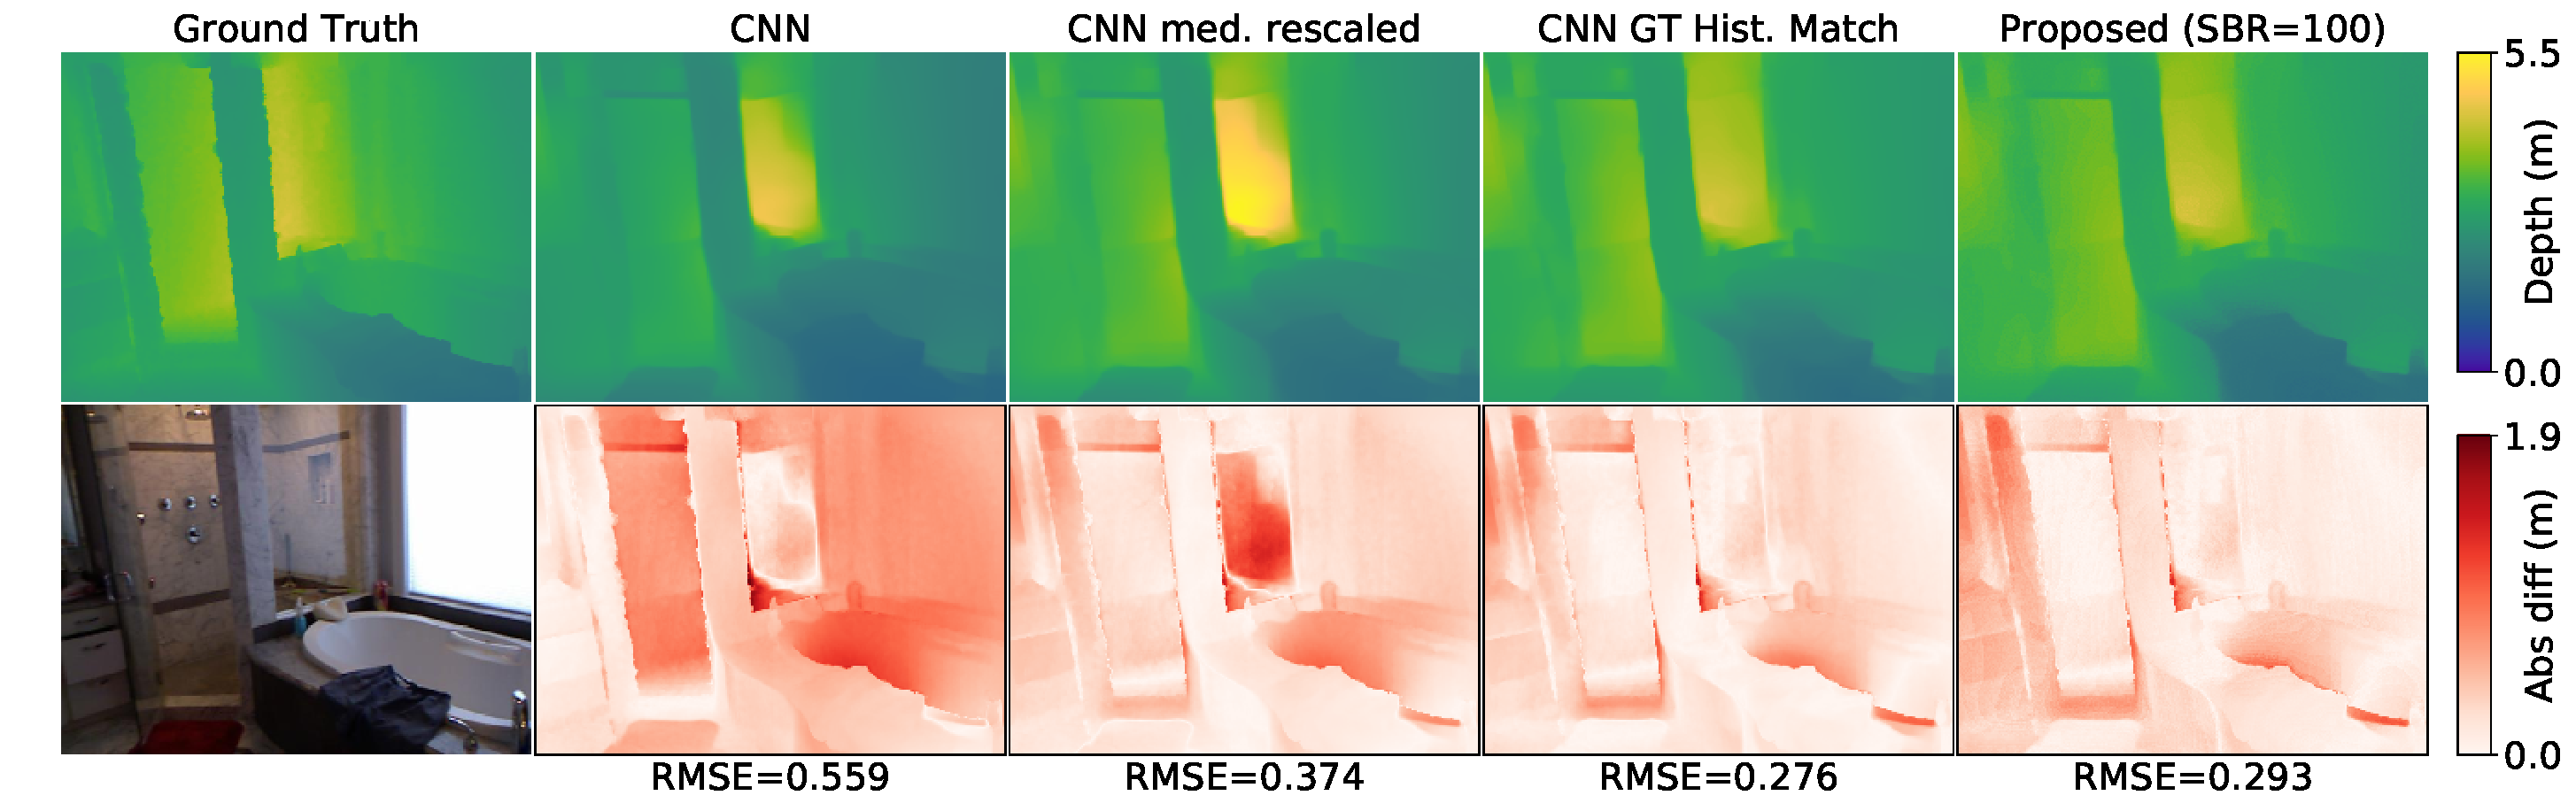
\includegraphics[width=\textwidth]{sections/figures/comparison/densedepth_285_comparison.png}
  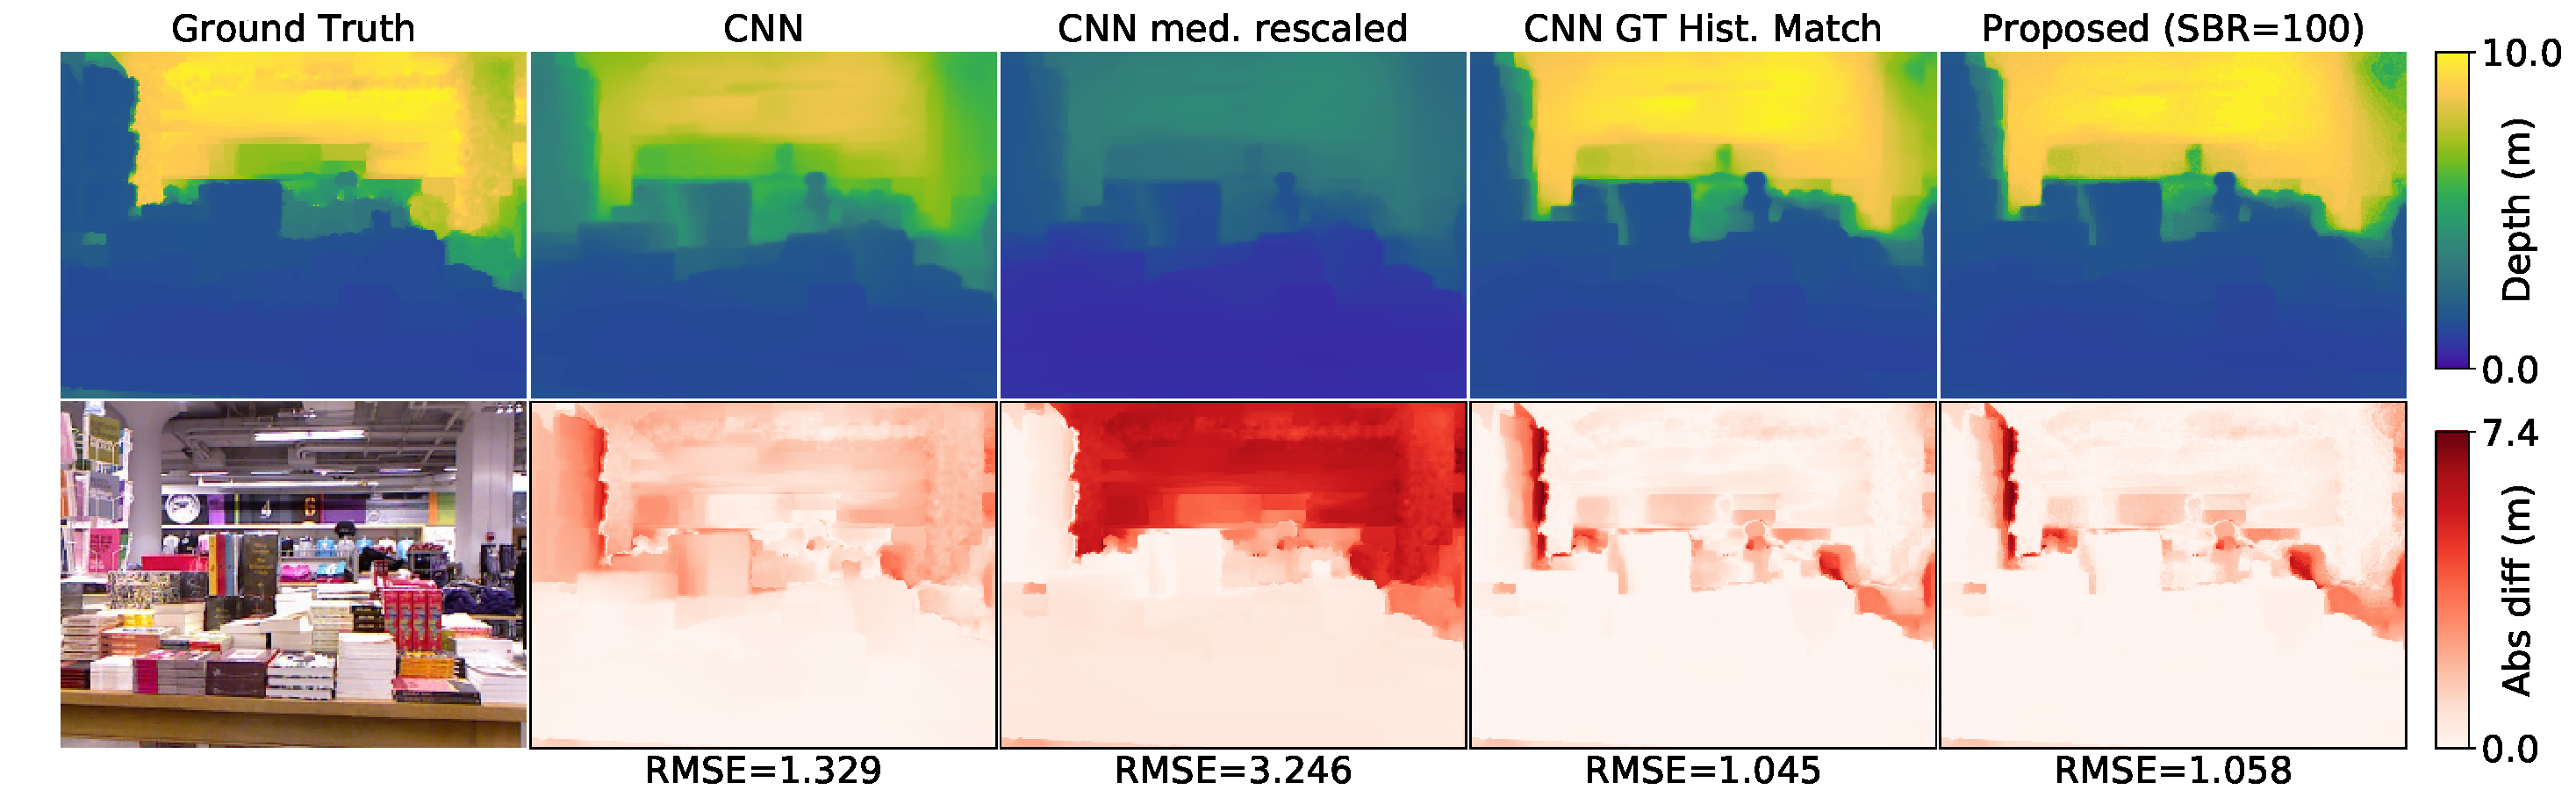
\includegraphics[width=\textwidth]{sections/figures/comparison/densedepth_42_comparison.png}
  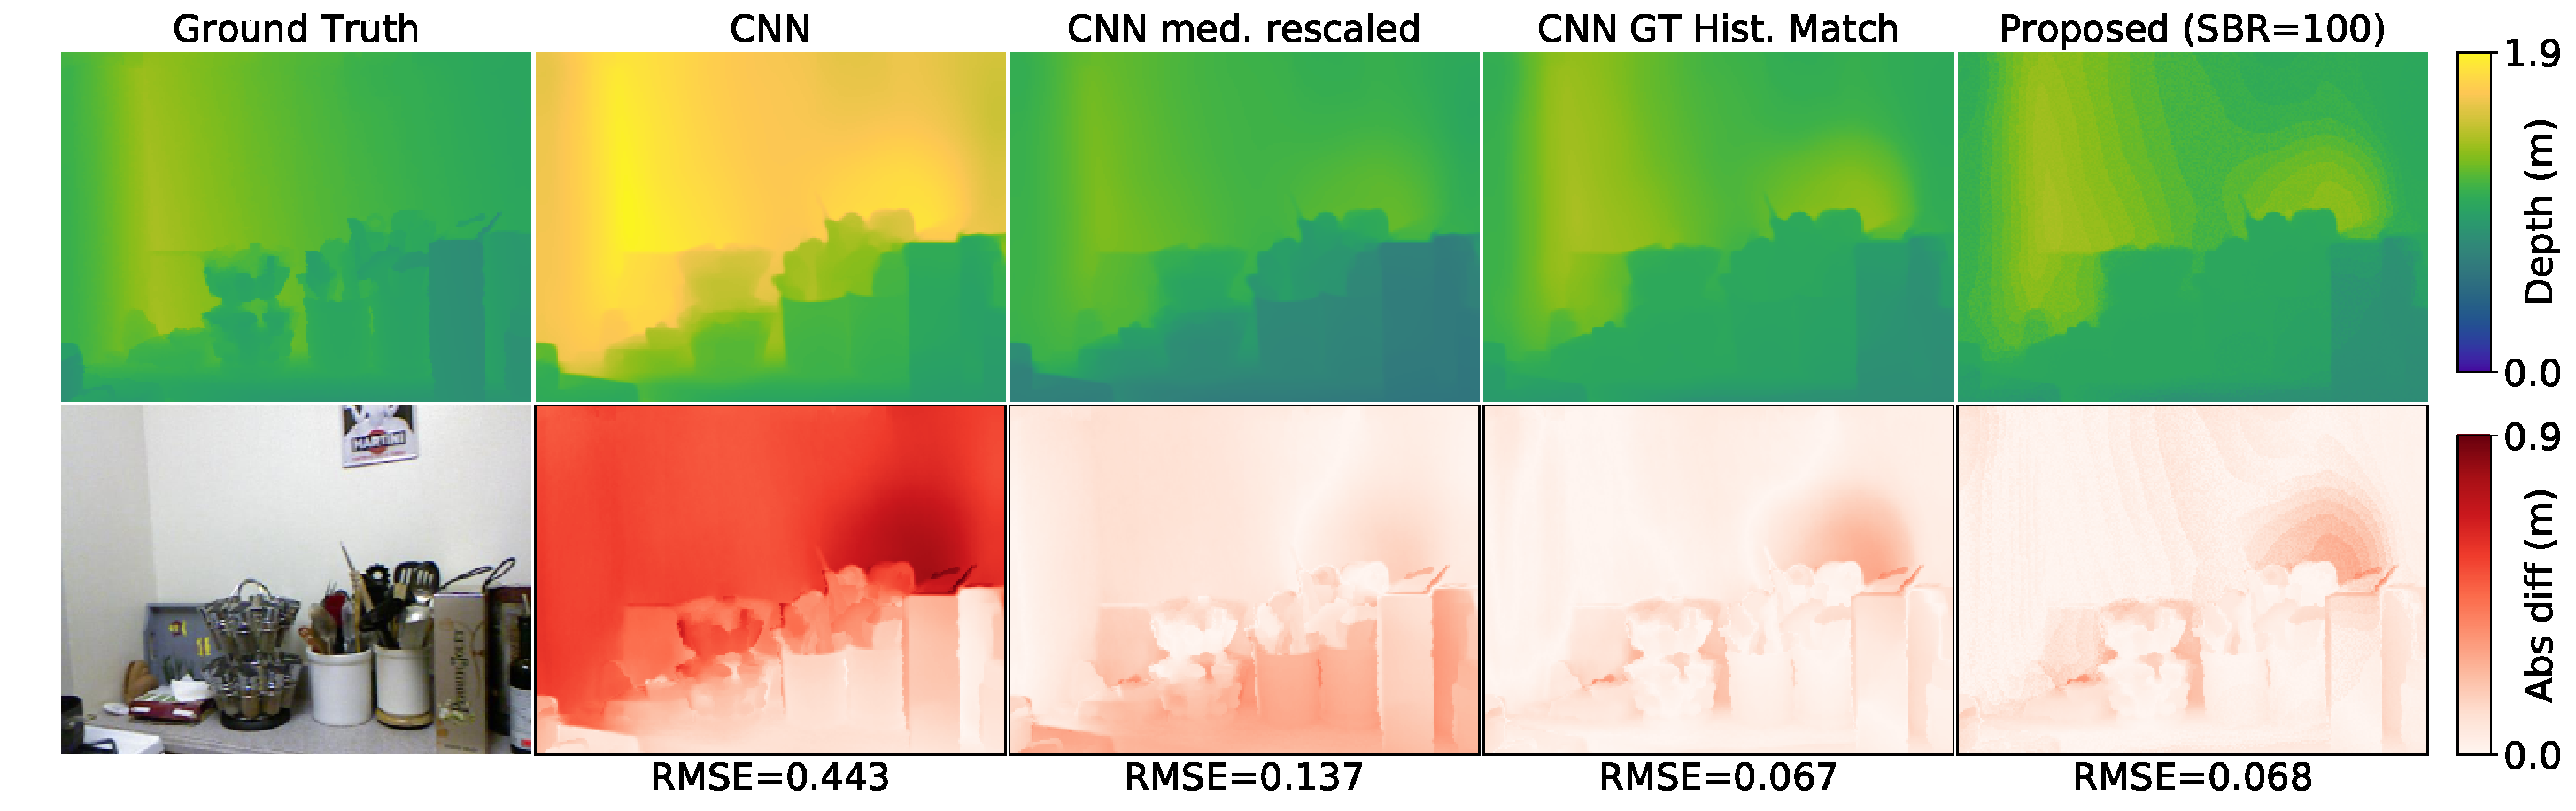
\includegraphics[width=\textwidth]{sections/figures/comparison/densedepth_52_comparison.png}
  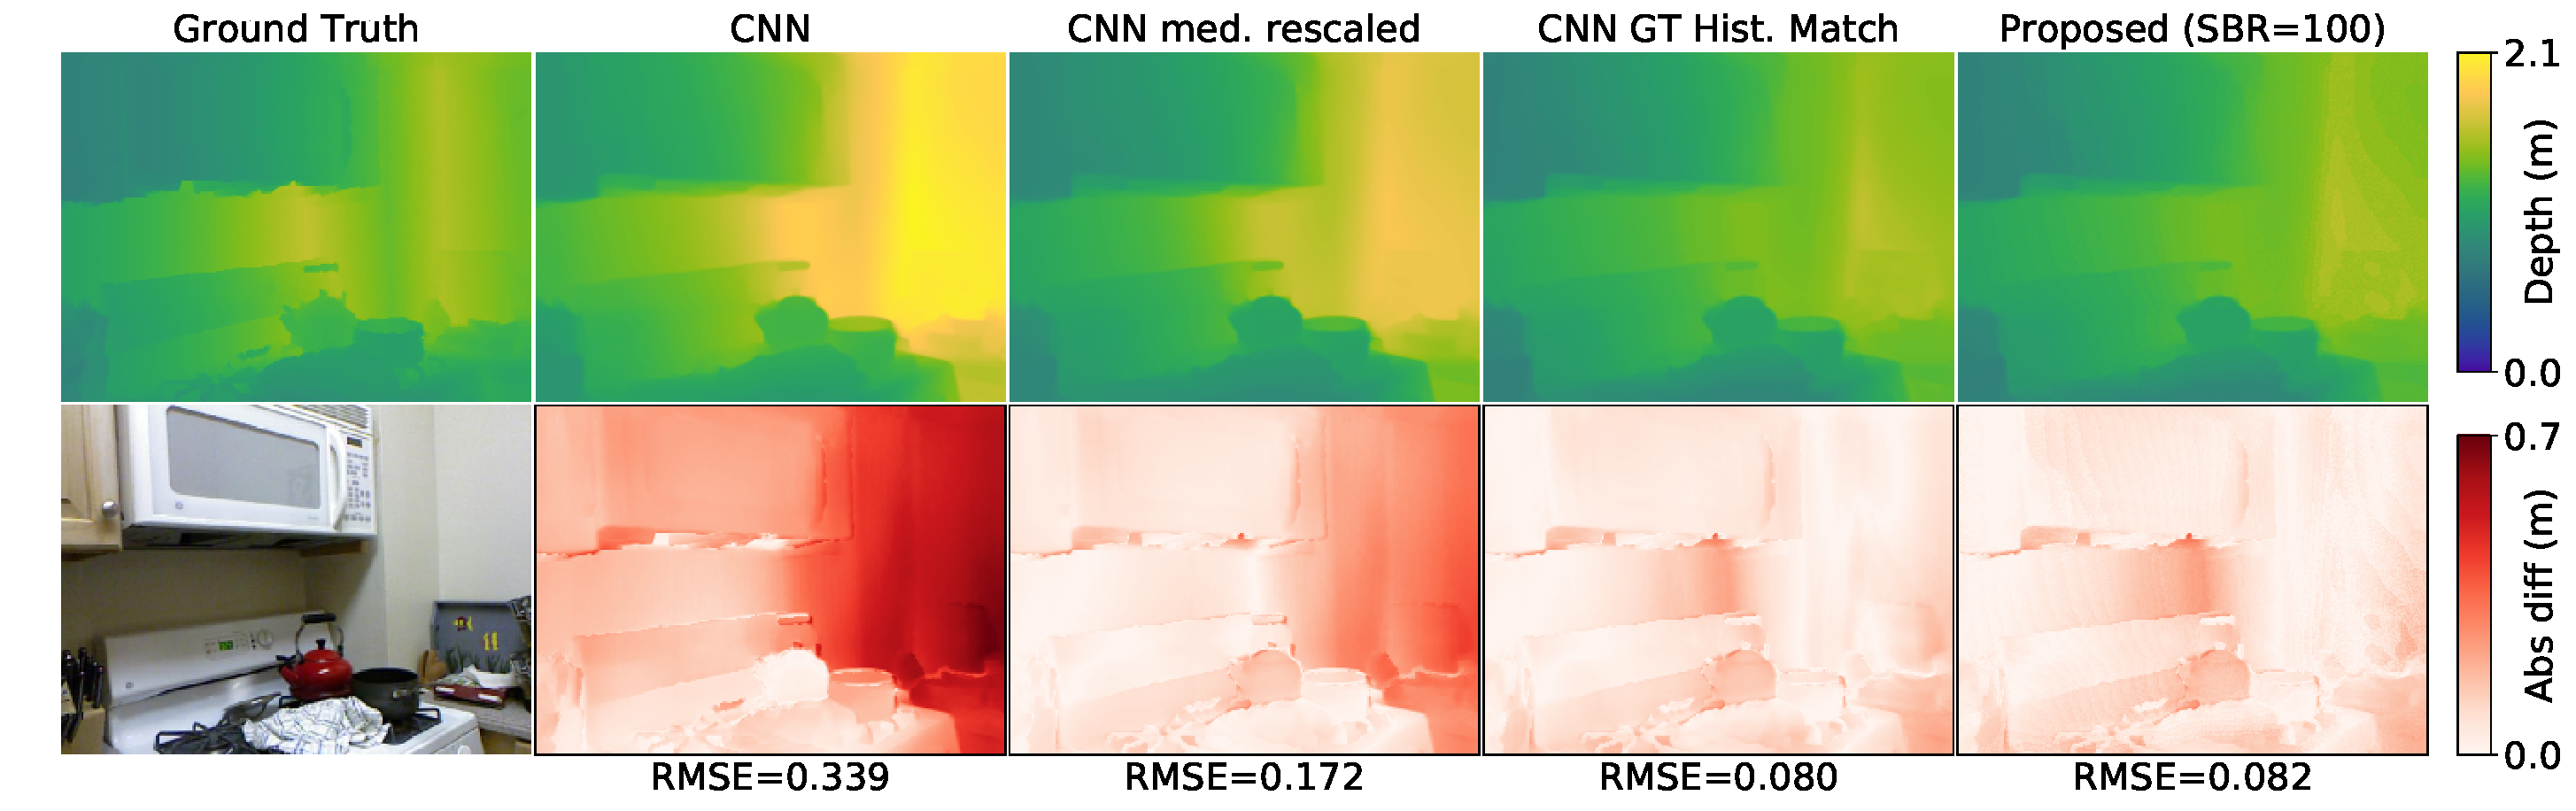
\includegraphics[width=\textwidth]{sections/figures/comparison/densedepth_53_comparison.png}
  \caption{Results on DenseDepth}
\end{figure*}
\begin{figure*}
  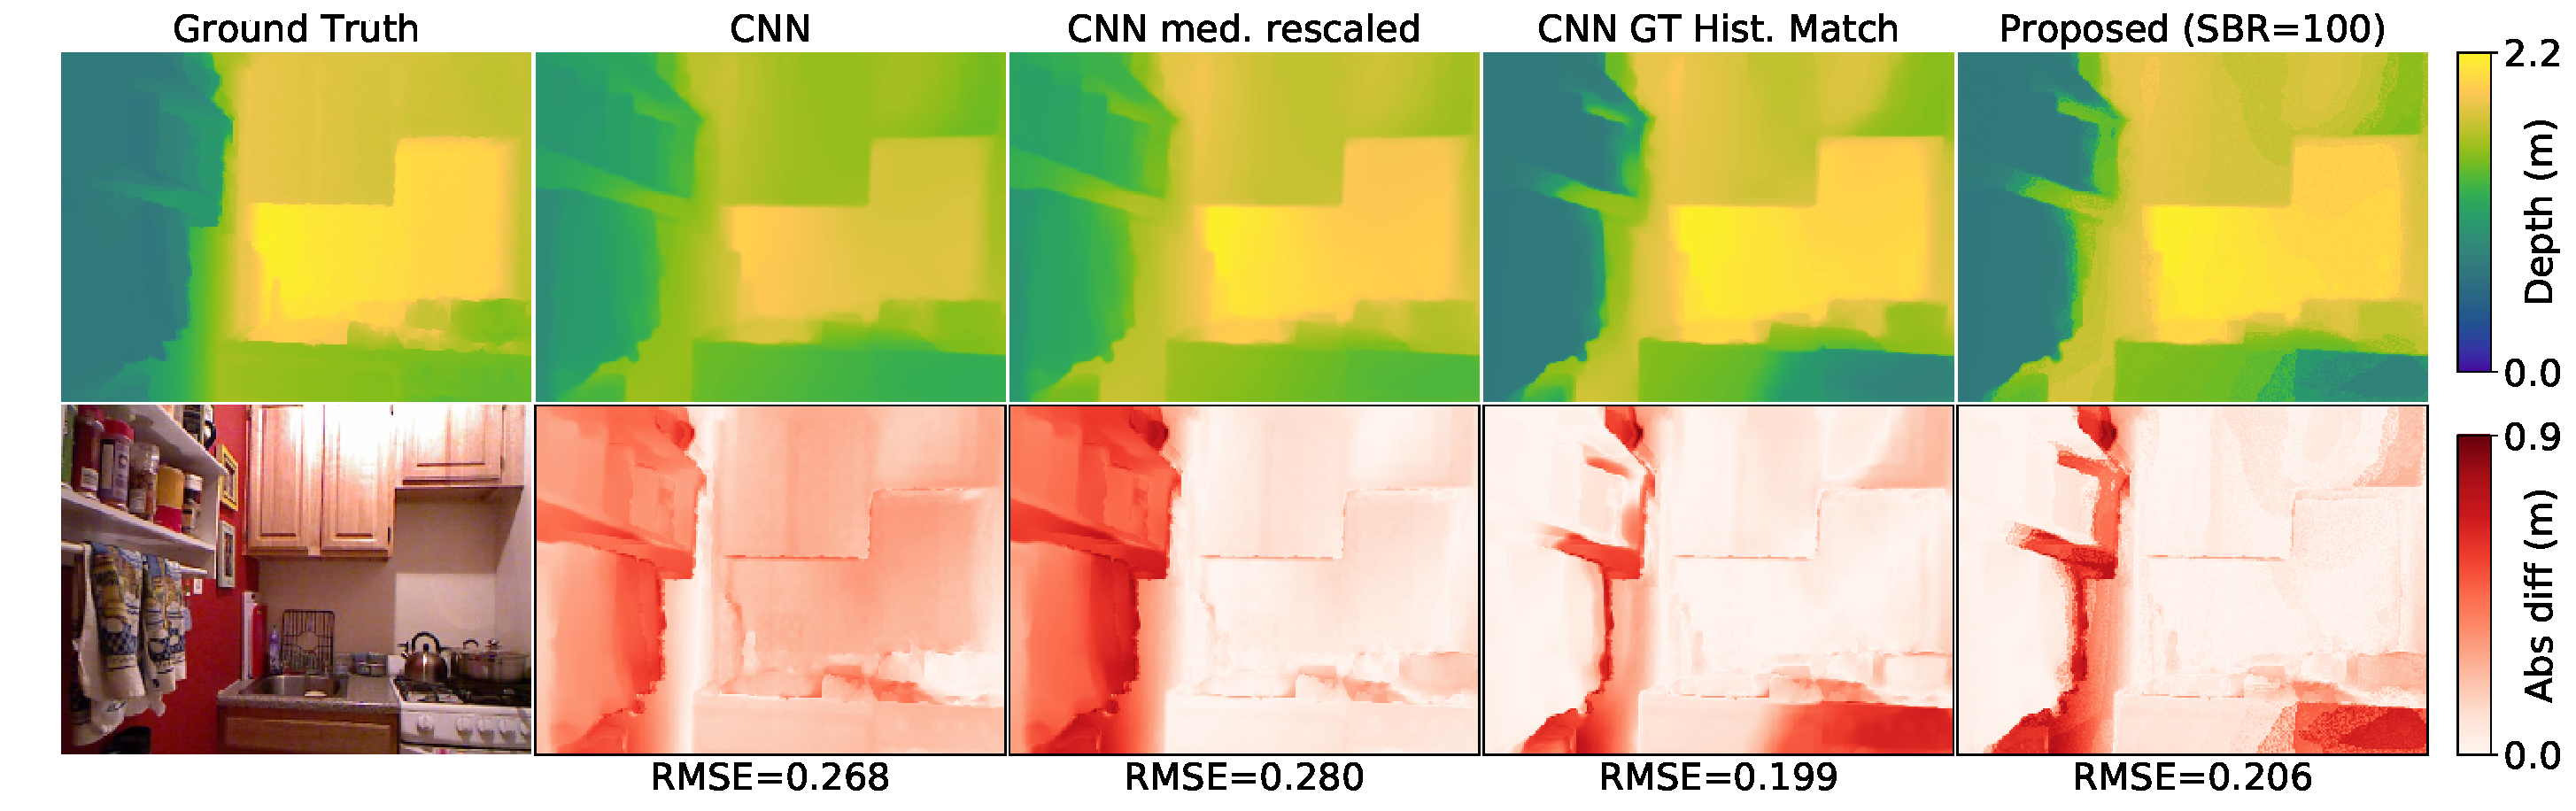
\includegraphics[width=\textwidth]{sections/figures/comparison/densedepth_103_comparison.png}
  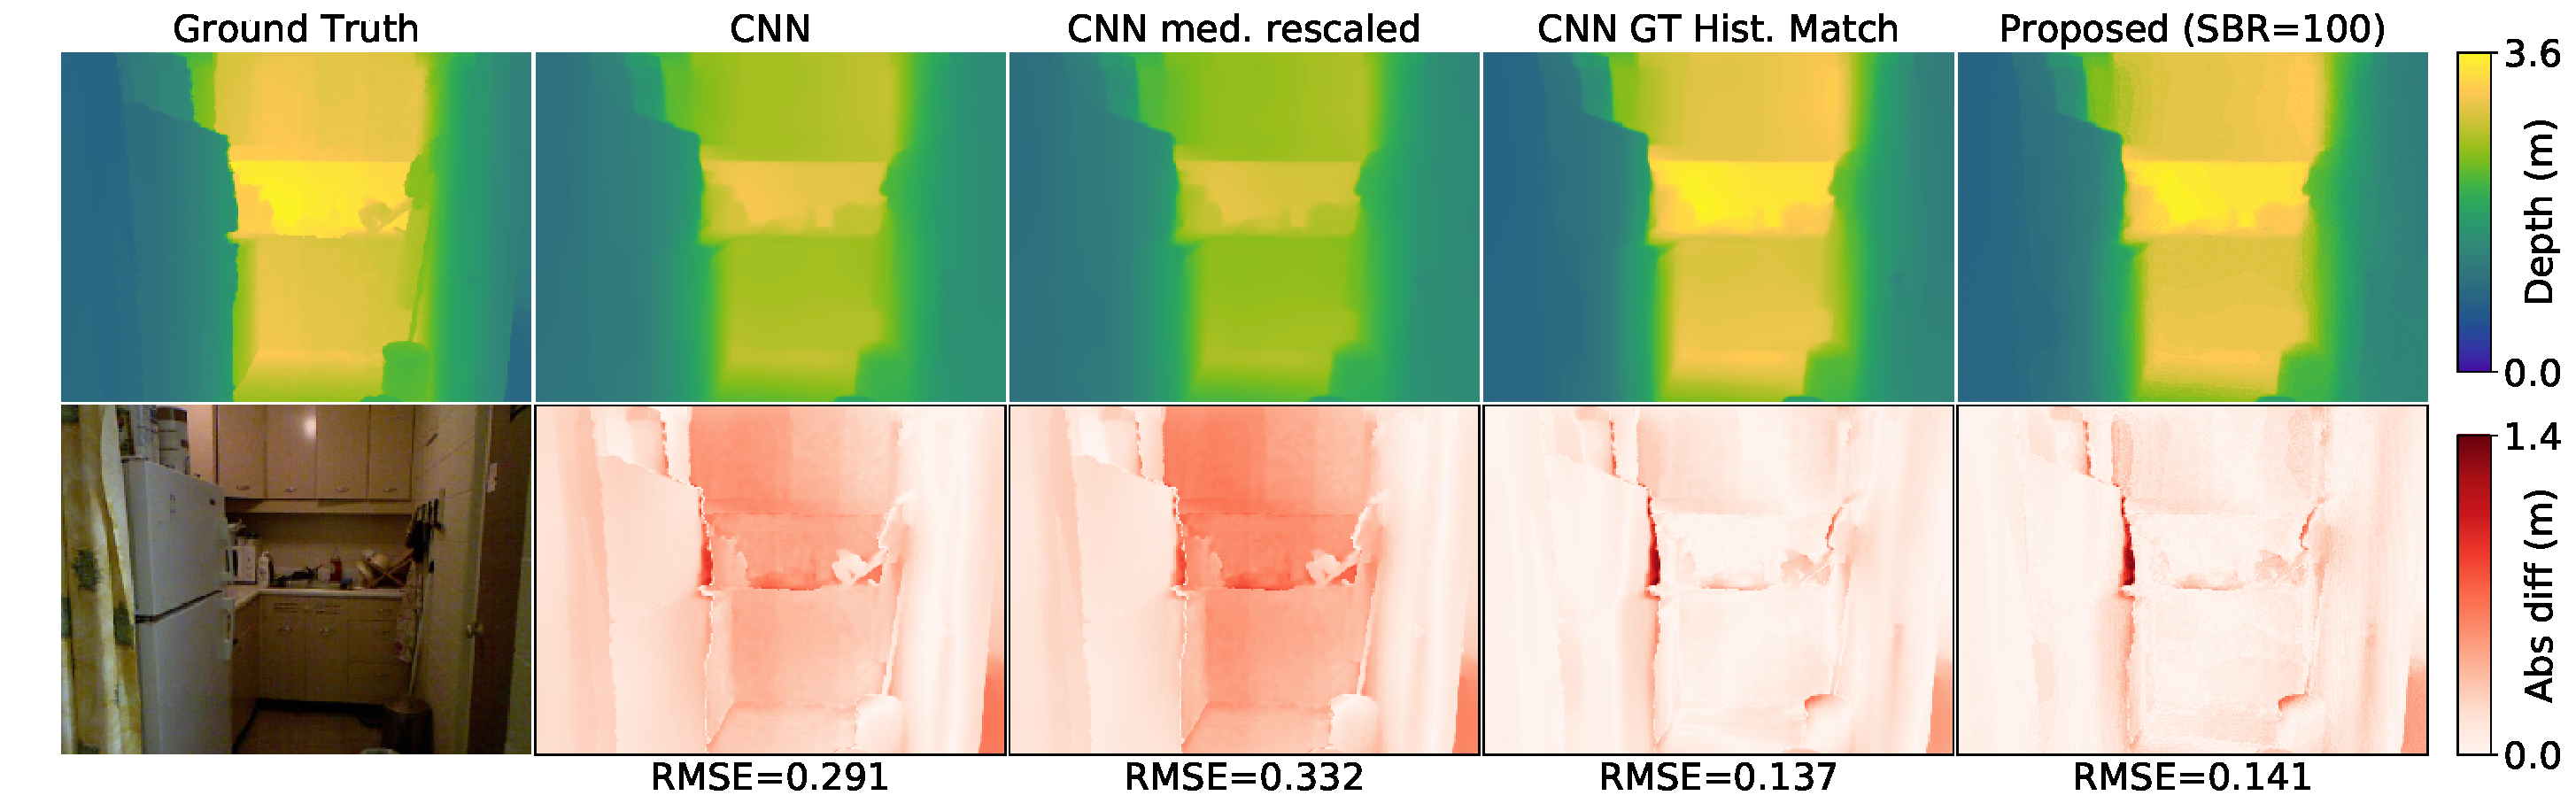
\includegraphics[width=\textwidth]{sections/figures/comparison/densedepth_224_comparison.png}
  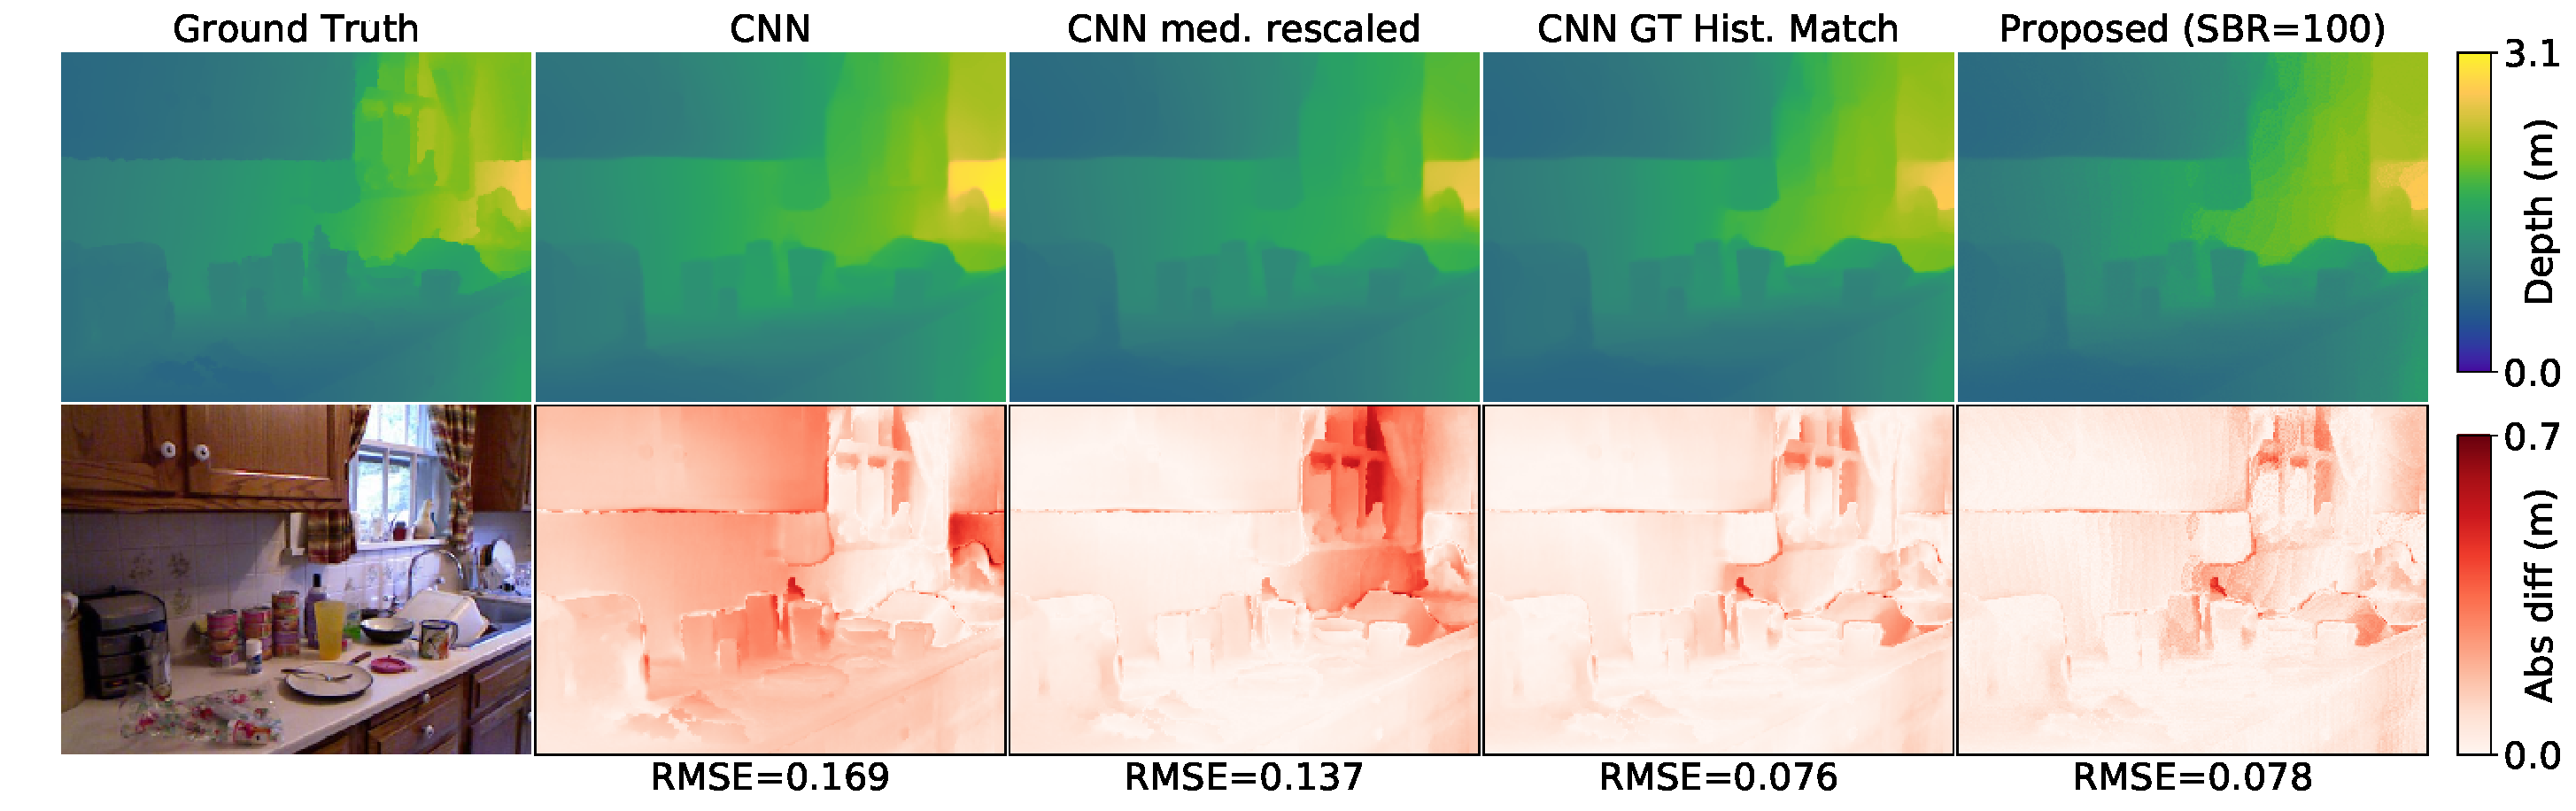
\includegraphics[width=\textwidth]{sections/figures/comparison/densedepth_226_comparison.png}
  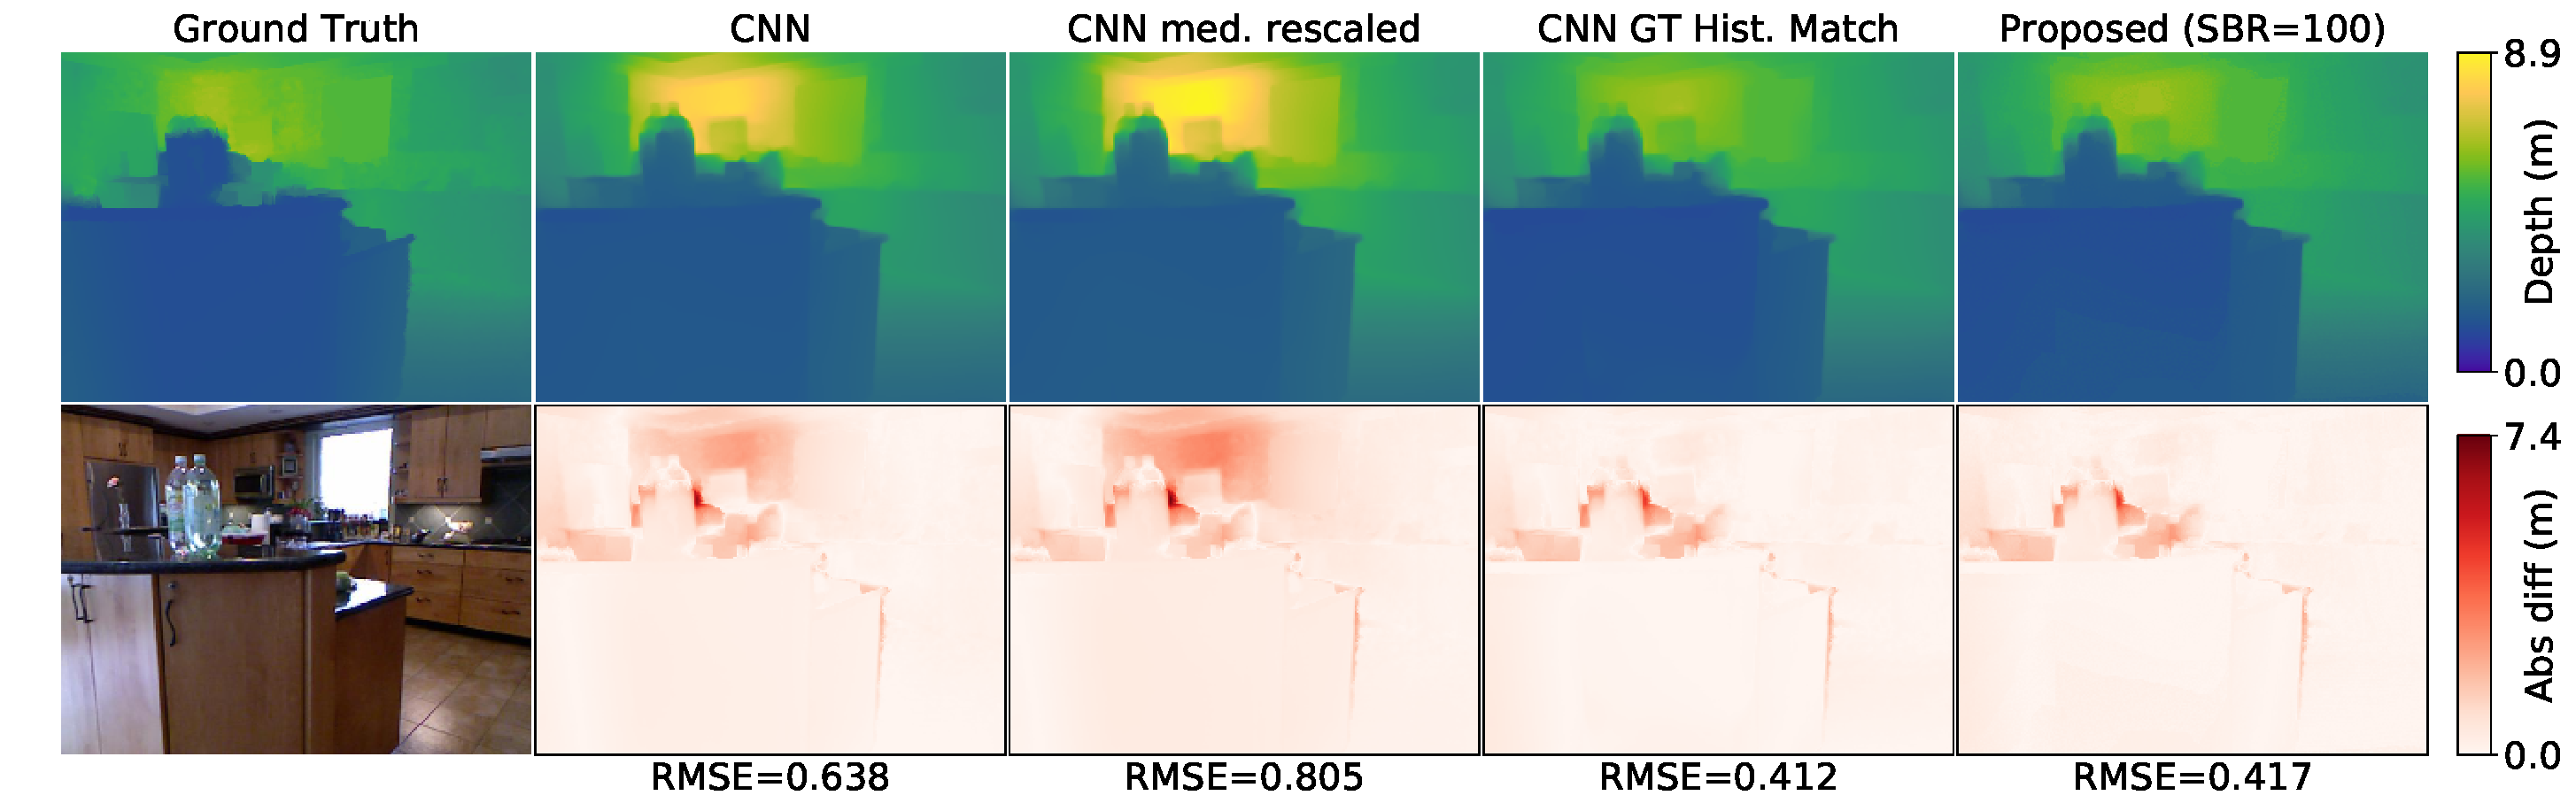
\includegraphics[width=\textwidth]{sections/figures/comparison/densedepth_352_comparison.png}
  \caption{Results on DenseDepth}
\end{figure*}
\begin{figure*}
  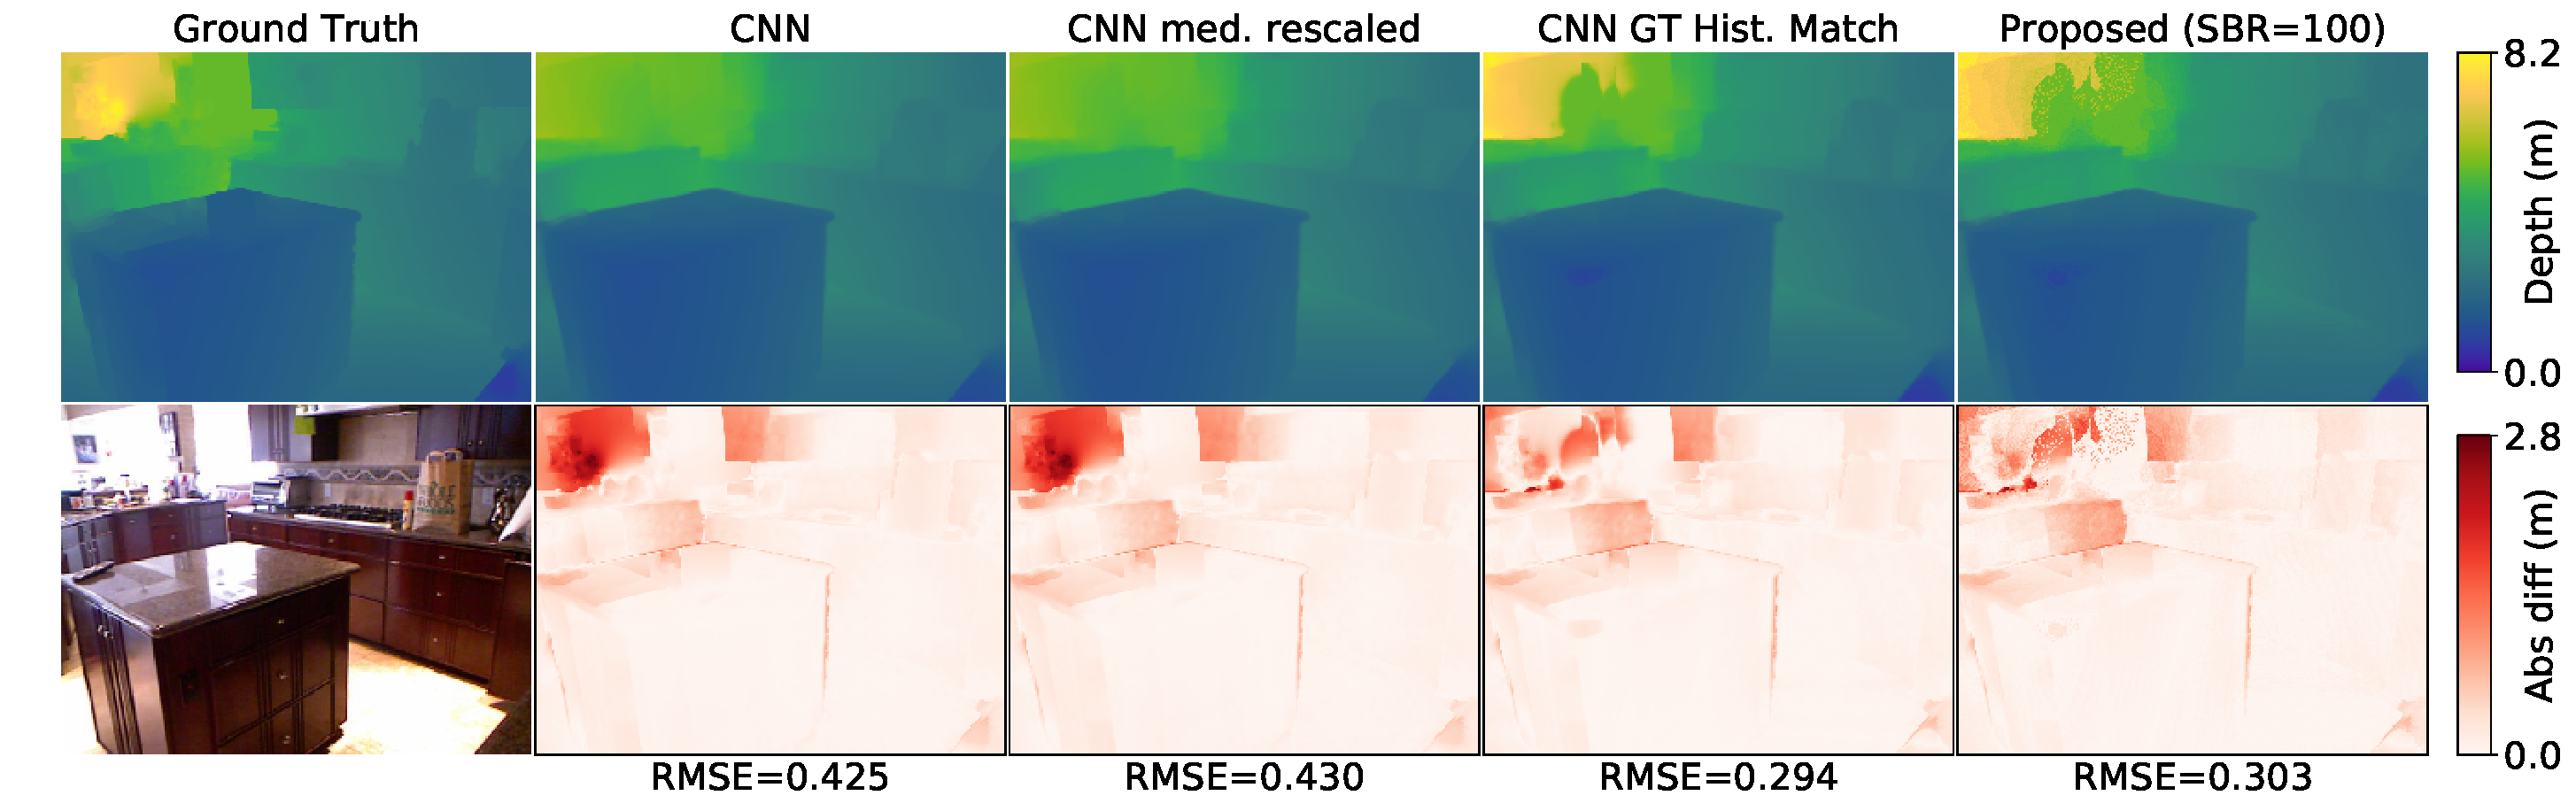
\includegraphics[width=\textwidth]{sections/figures/comparison/densedepth_362_comparison.png}
  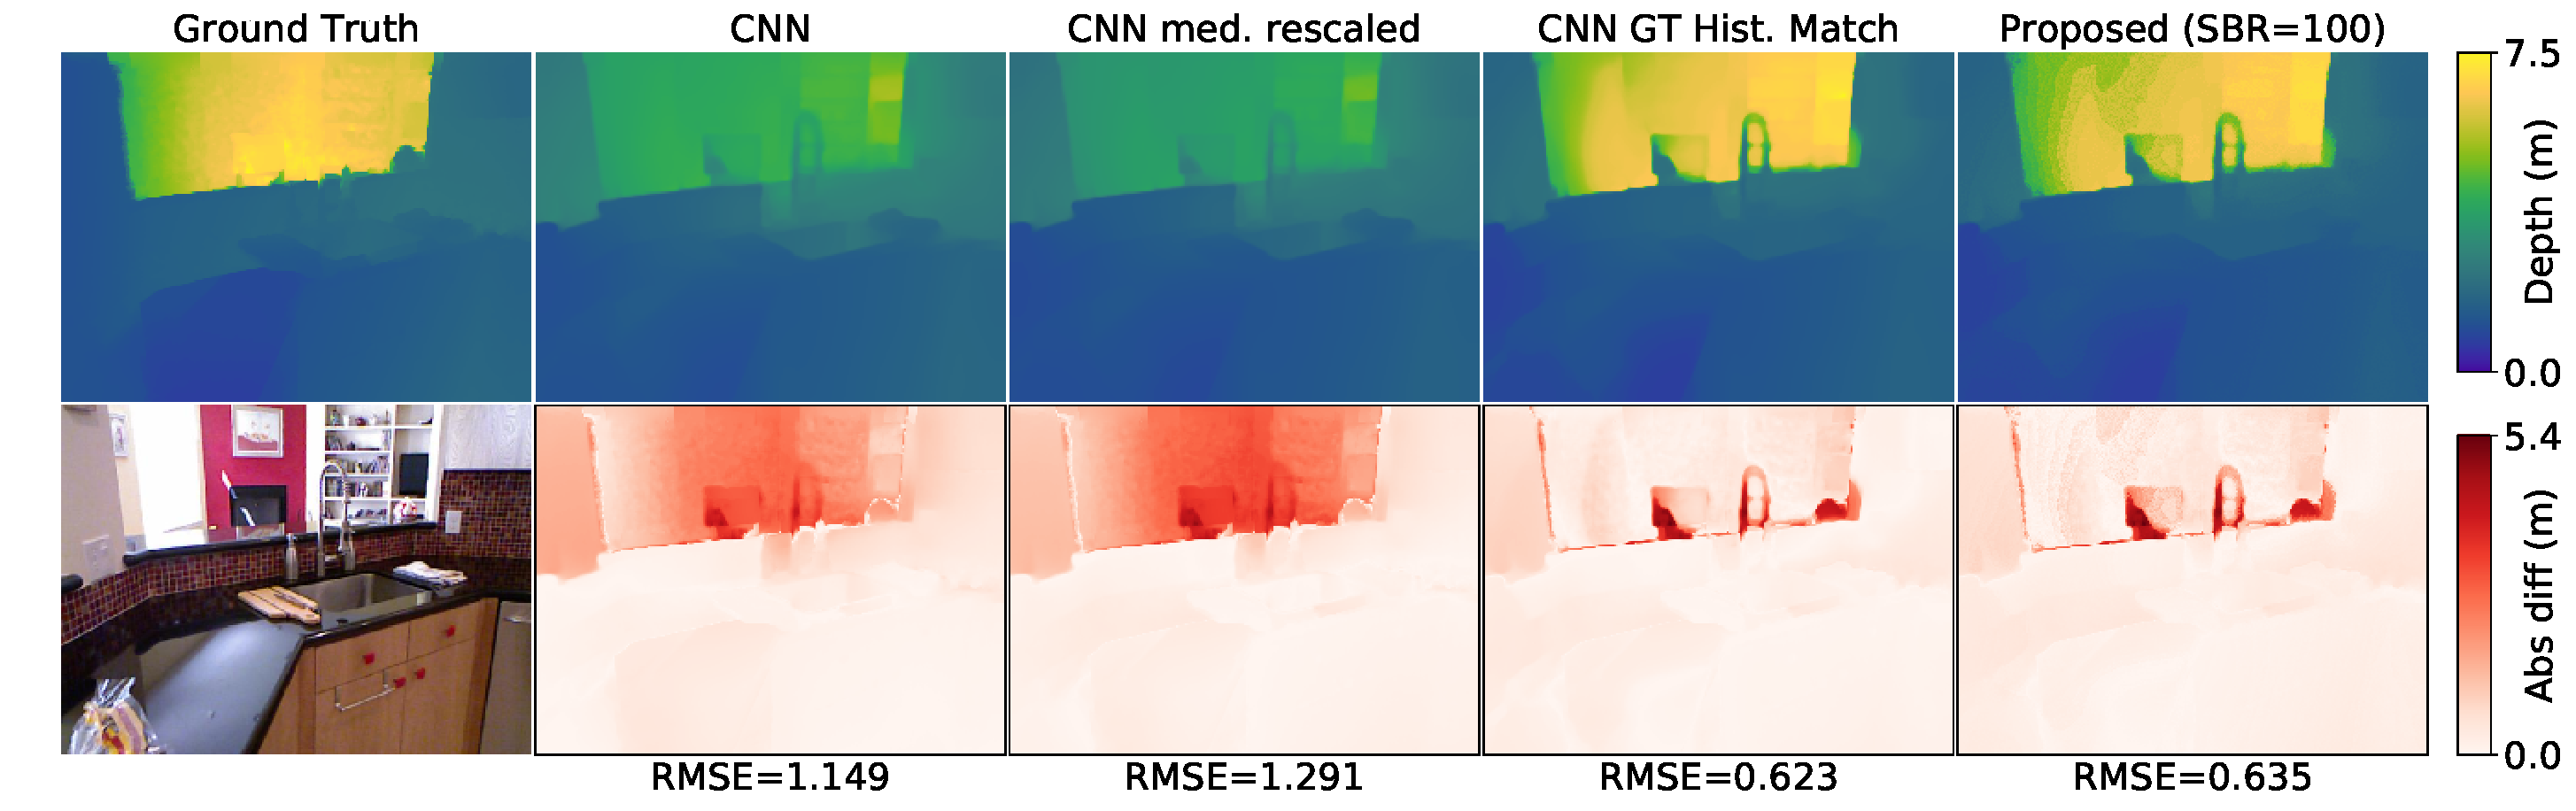
\includegraphics[width=\textwidth]{sections/figures/comparison/densedepth_379_comparison.png}
  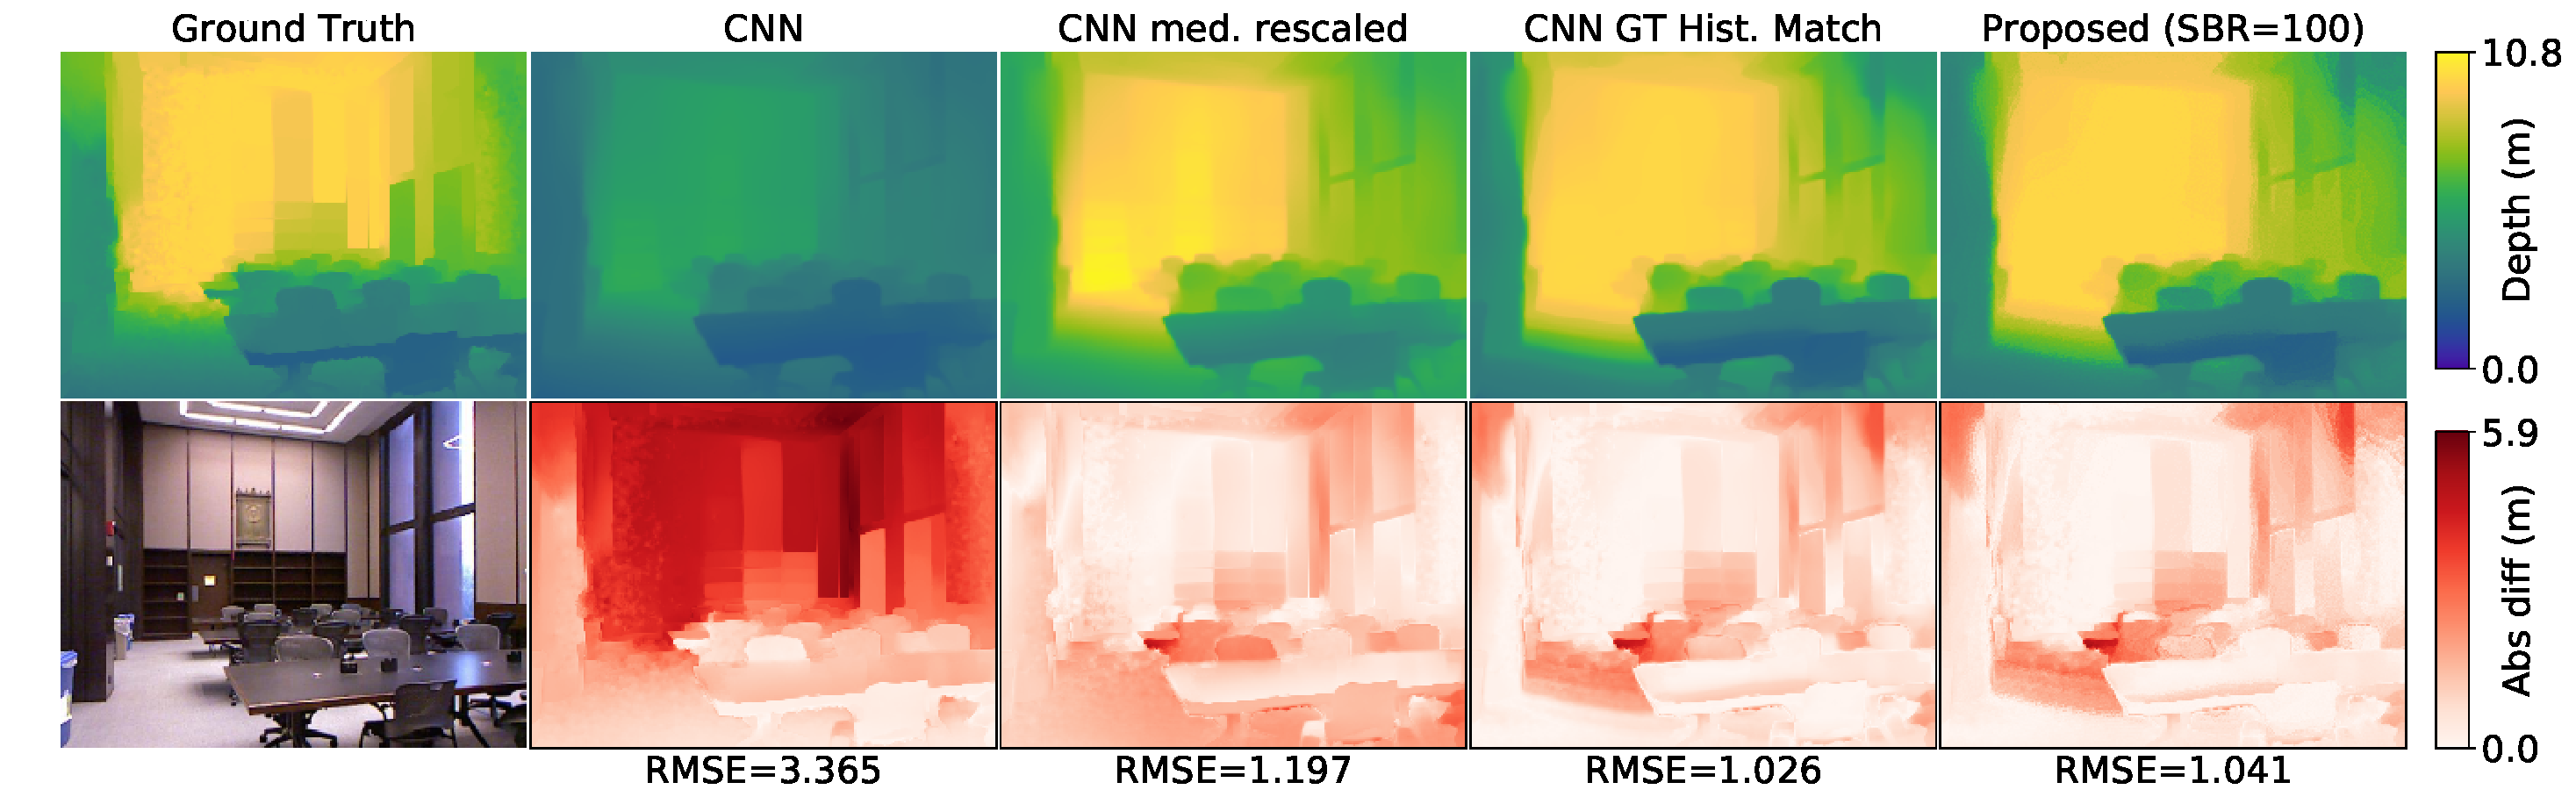
\includegraphics[width=\textwidth]{sections/figures/comparison/densedepth_107_comparison.png}
  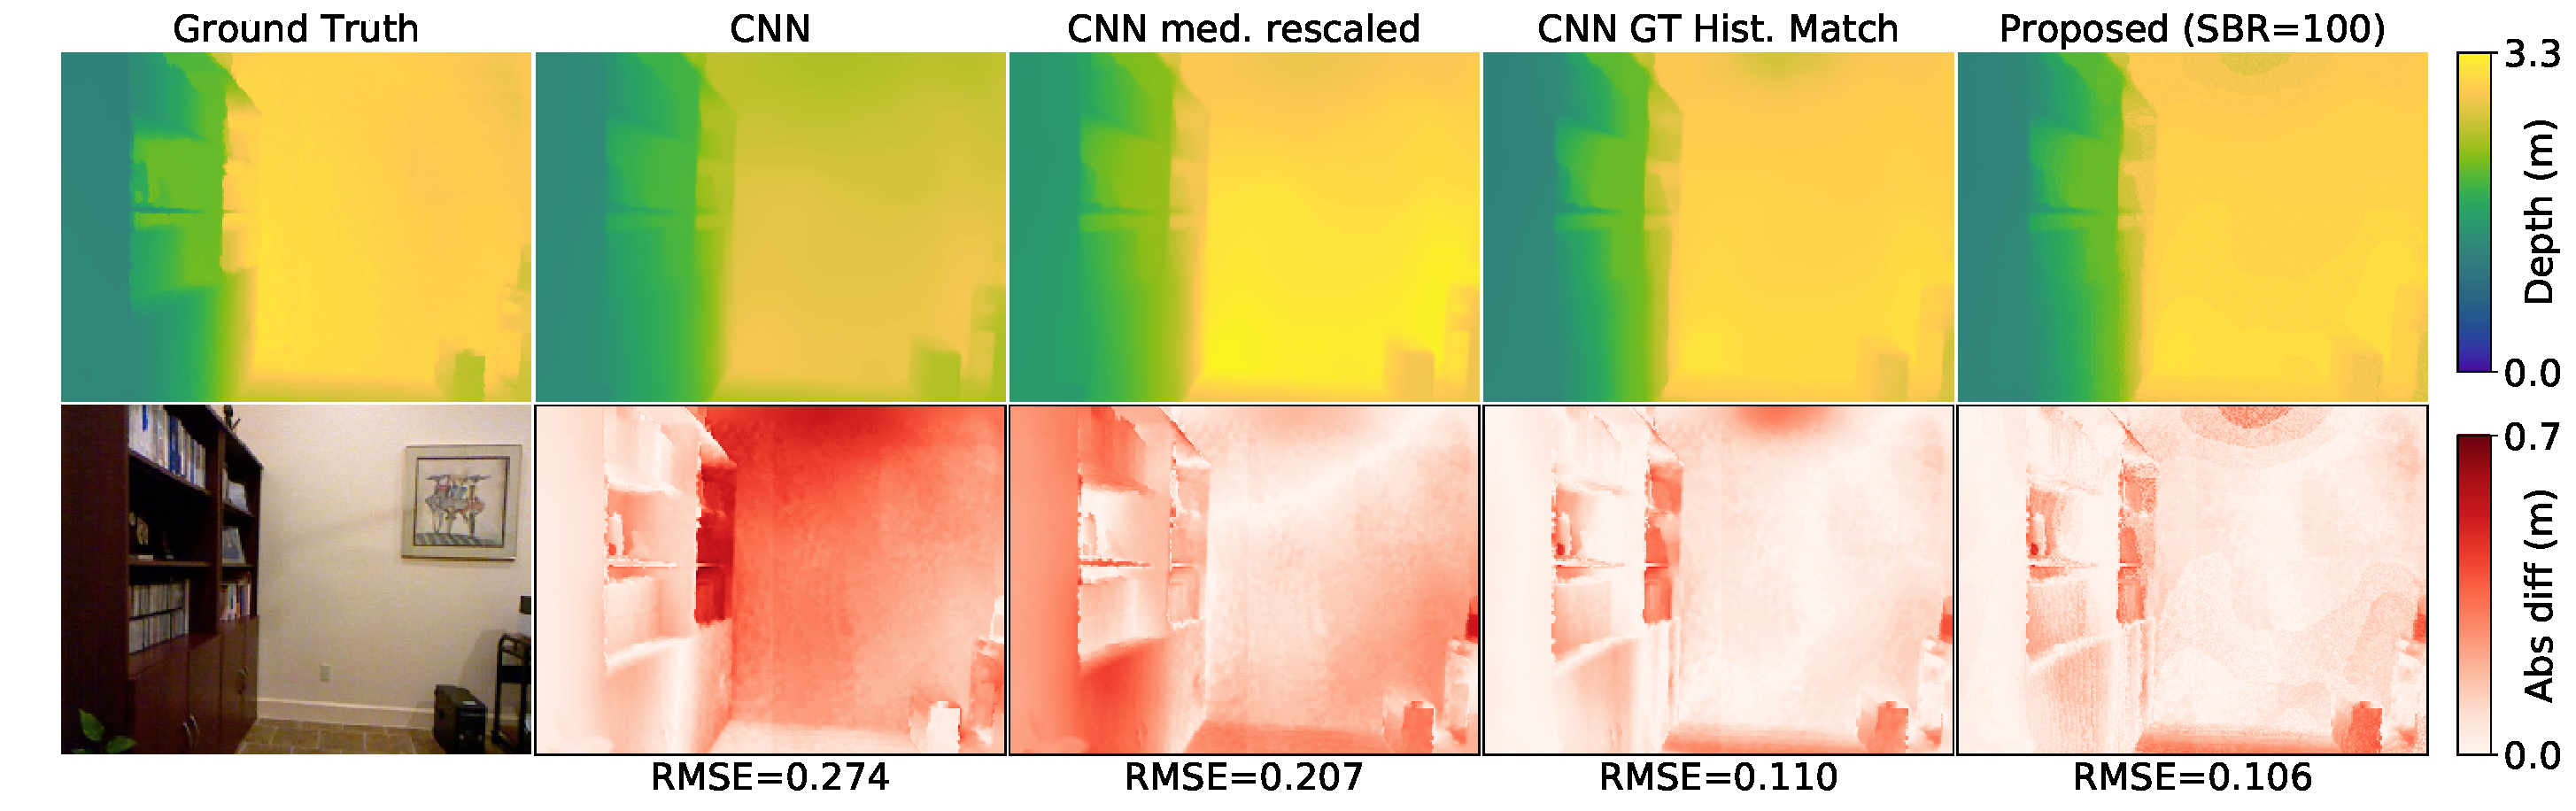
\includegraphics[width=\textwidth]{sections/figures/comparison/densedepth_187_comparison.png}
  \caption{Results on DenseDepth}
\end{figure*}
\begin{figure*}
  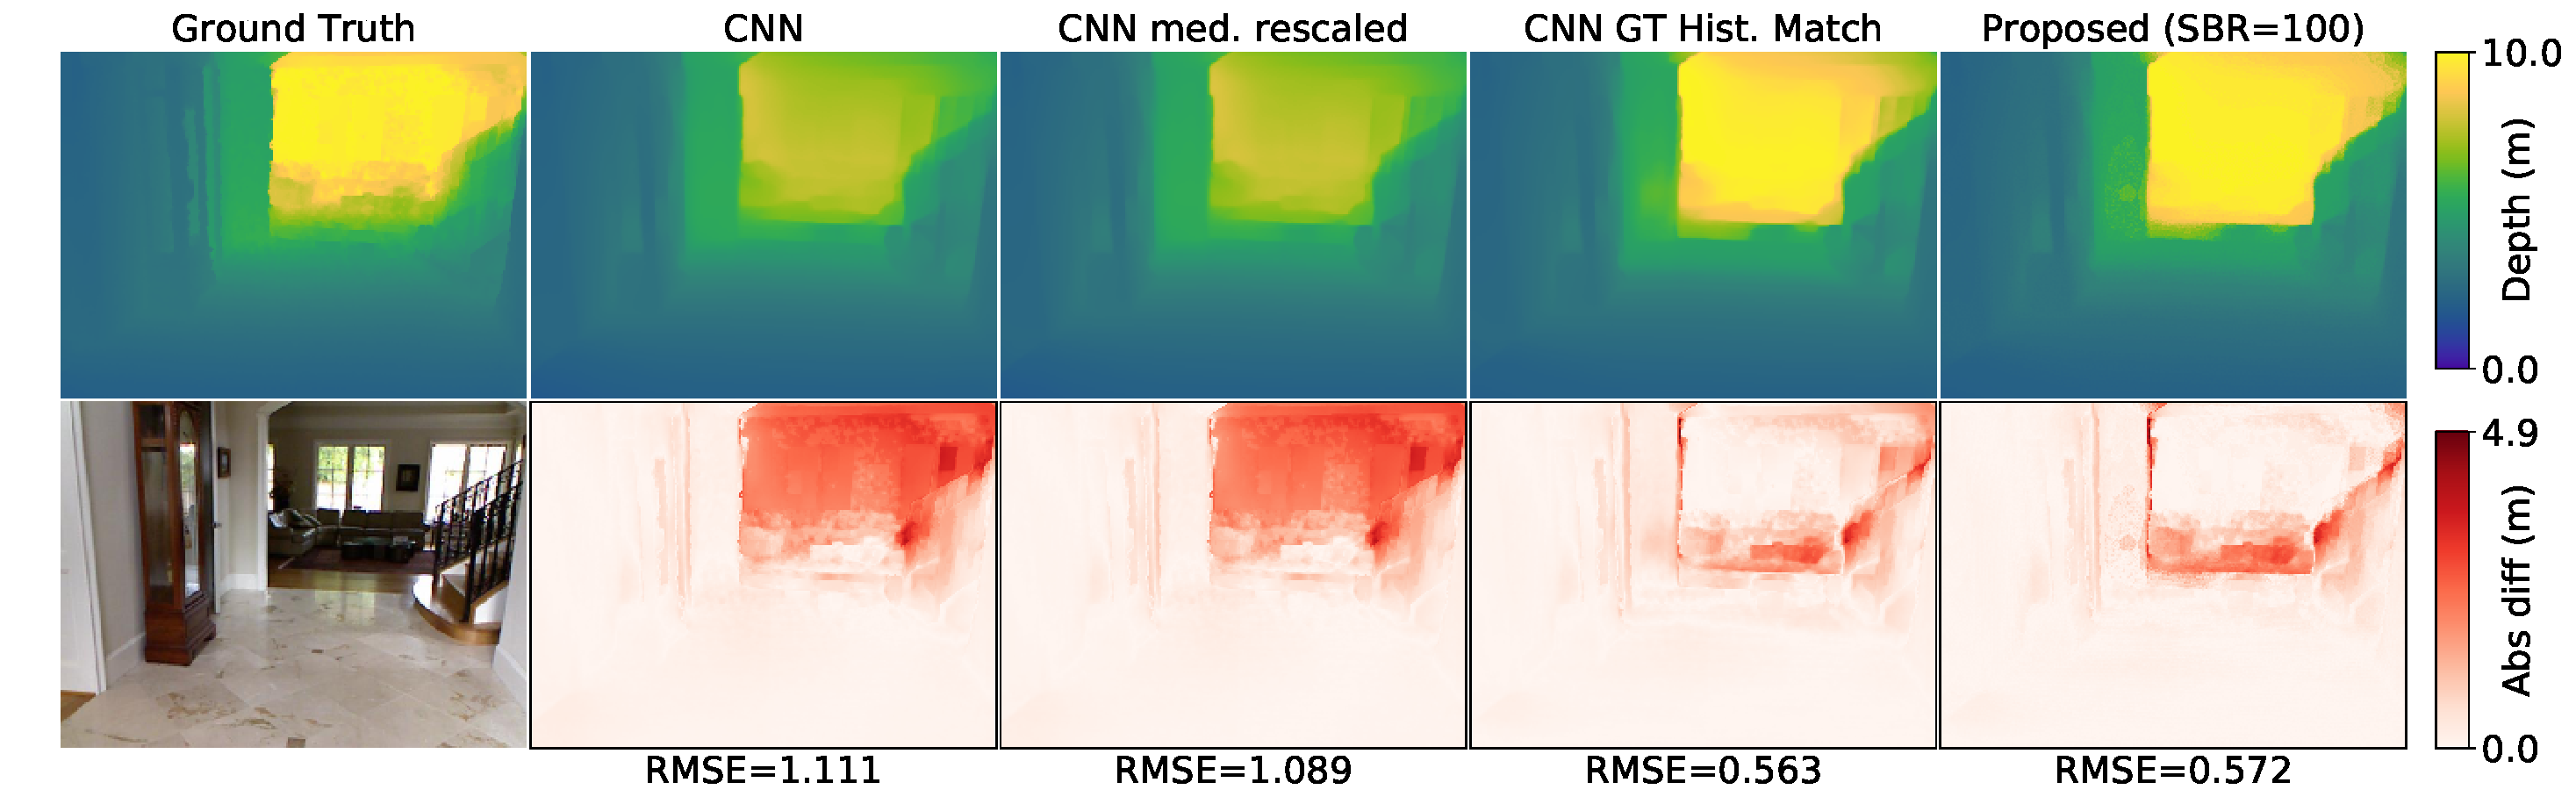
\includegraphics[width=\textwidth]{sections/figures/comparison/densedepth_140_comparison.png}
  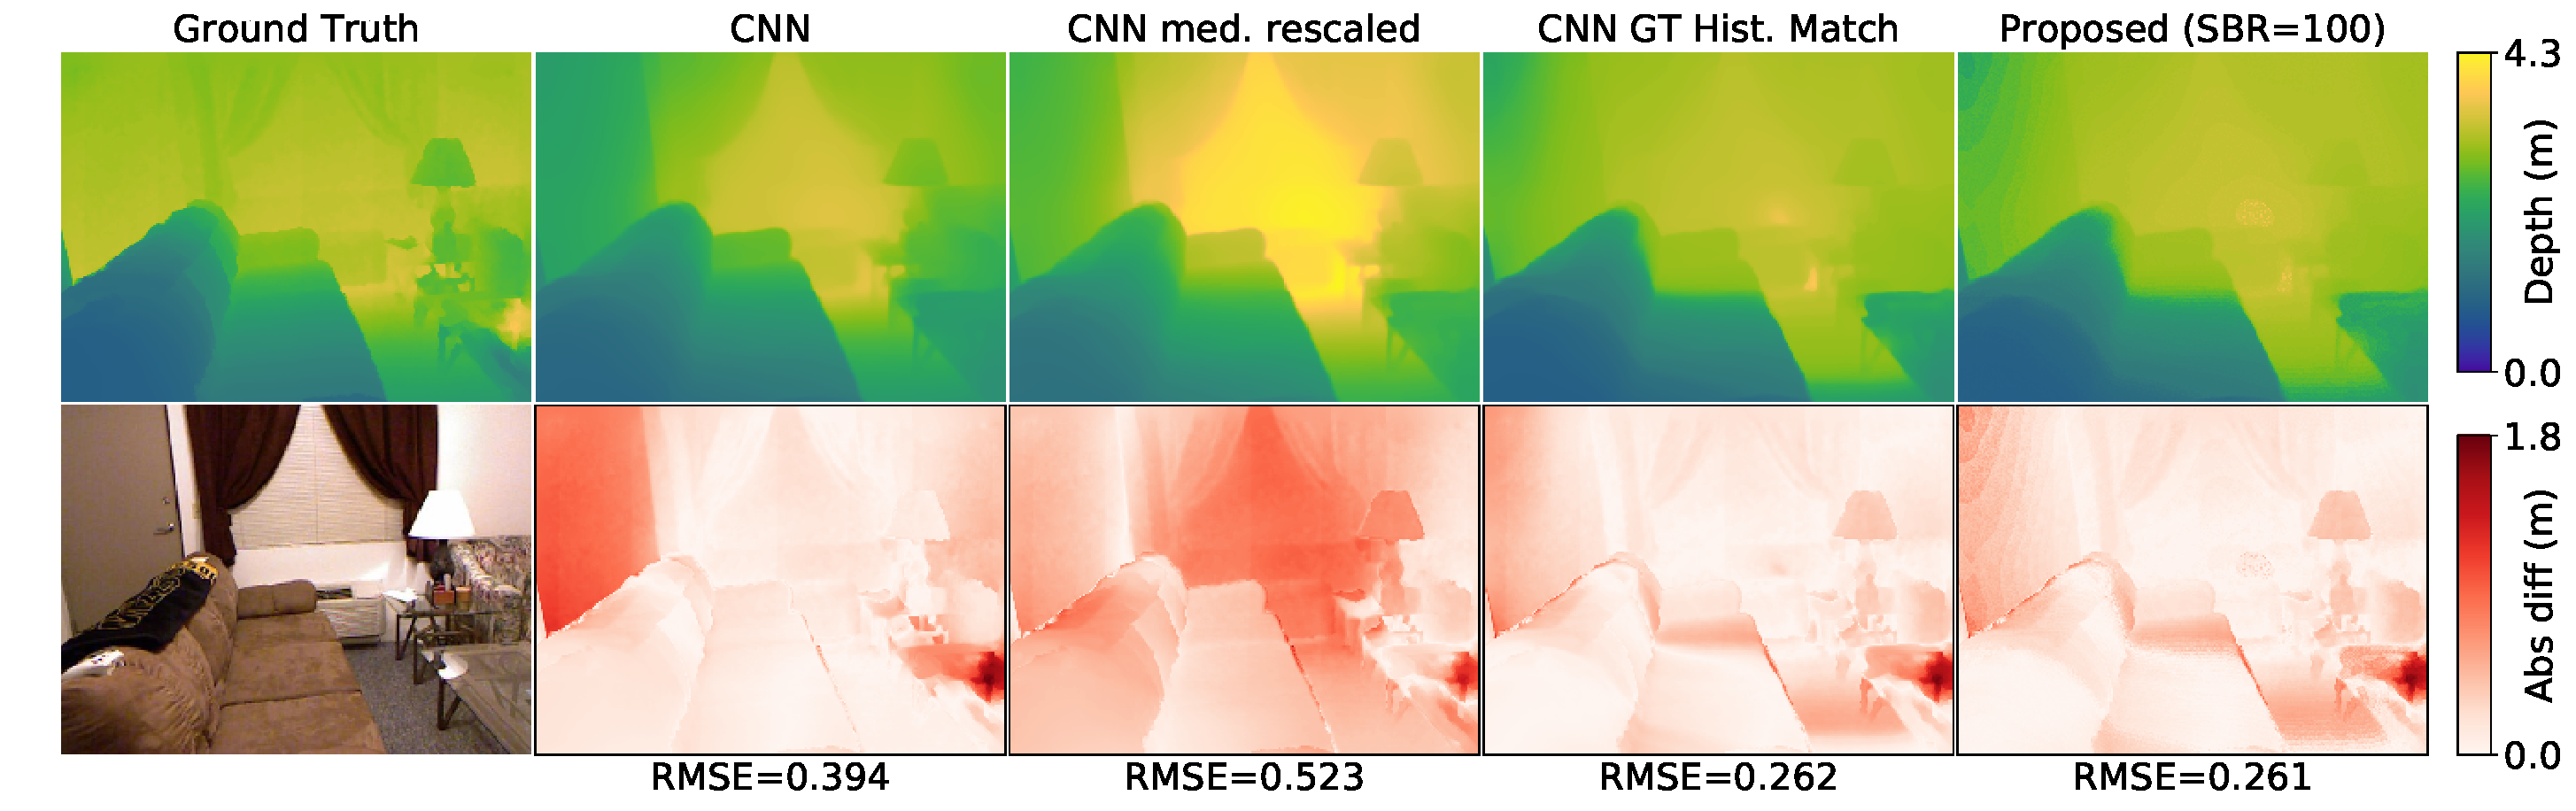
\includegraphics[width=\textwidth]{sections/figures/comparison/densedepth_244_comparison.png}
  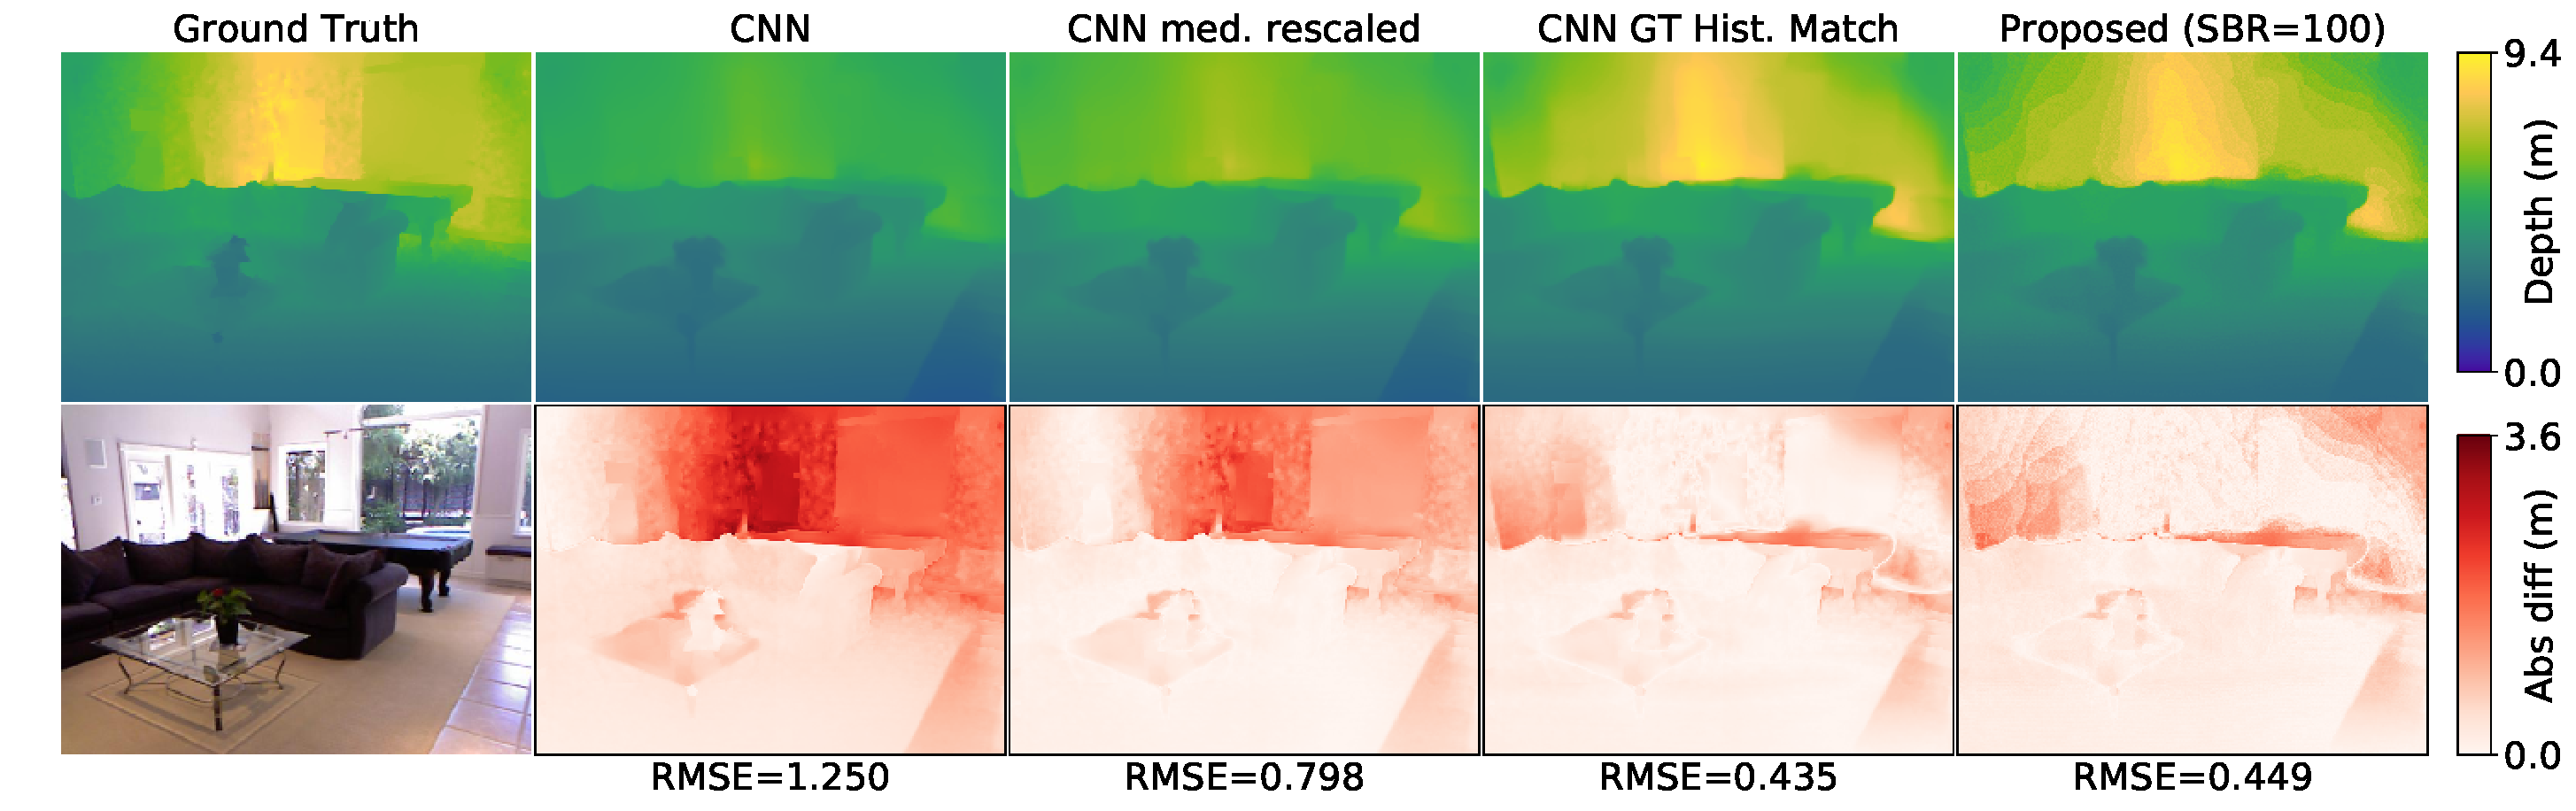
\includegraphics[width=\textwidth]{sections/figures/comparison/densedepth_527_comparison.png}
  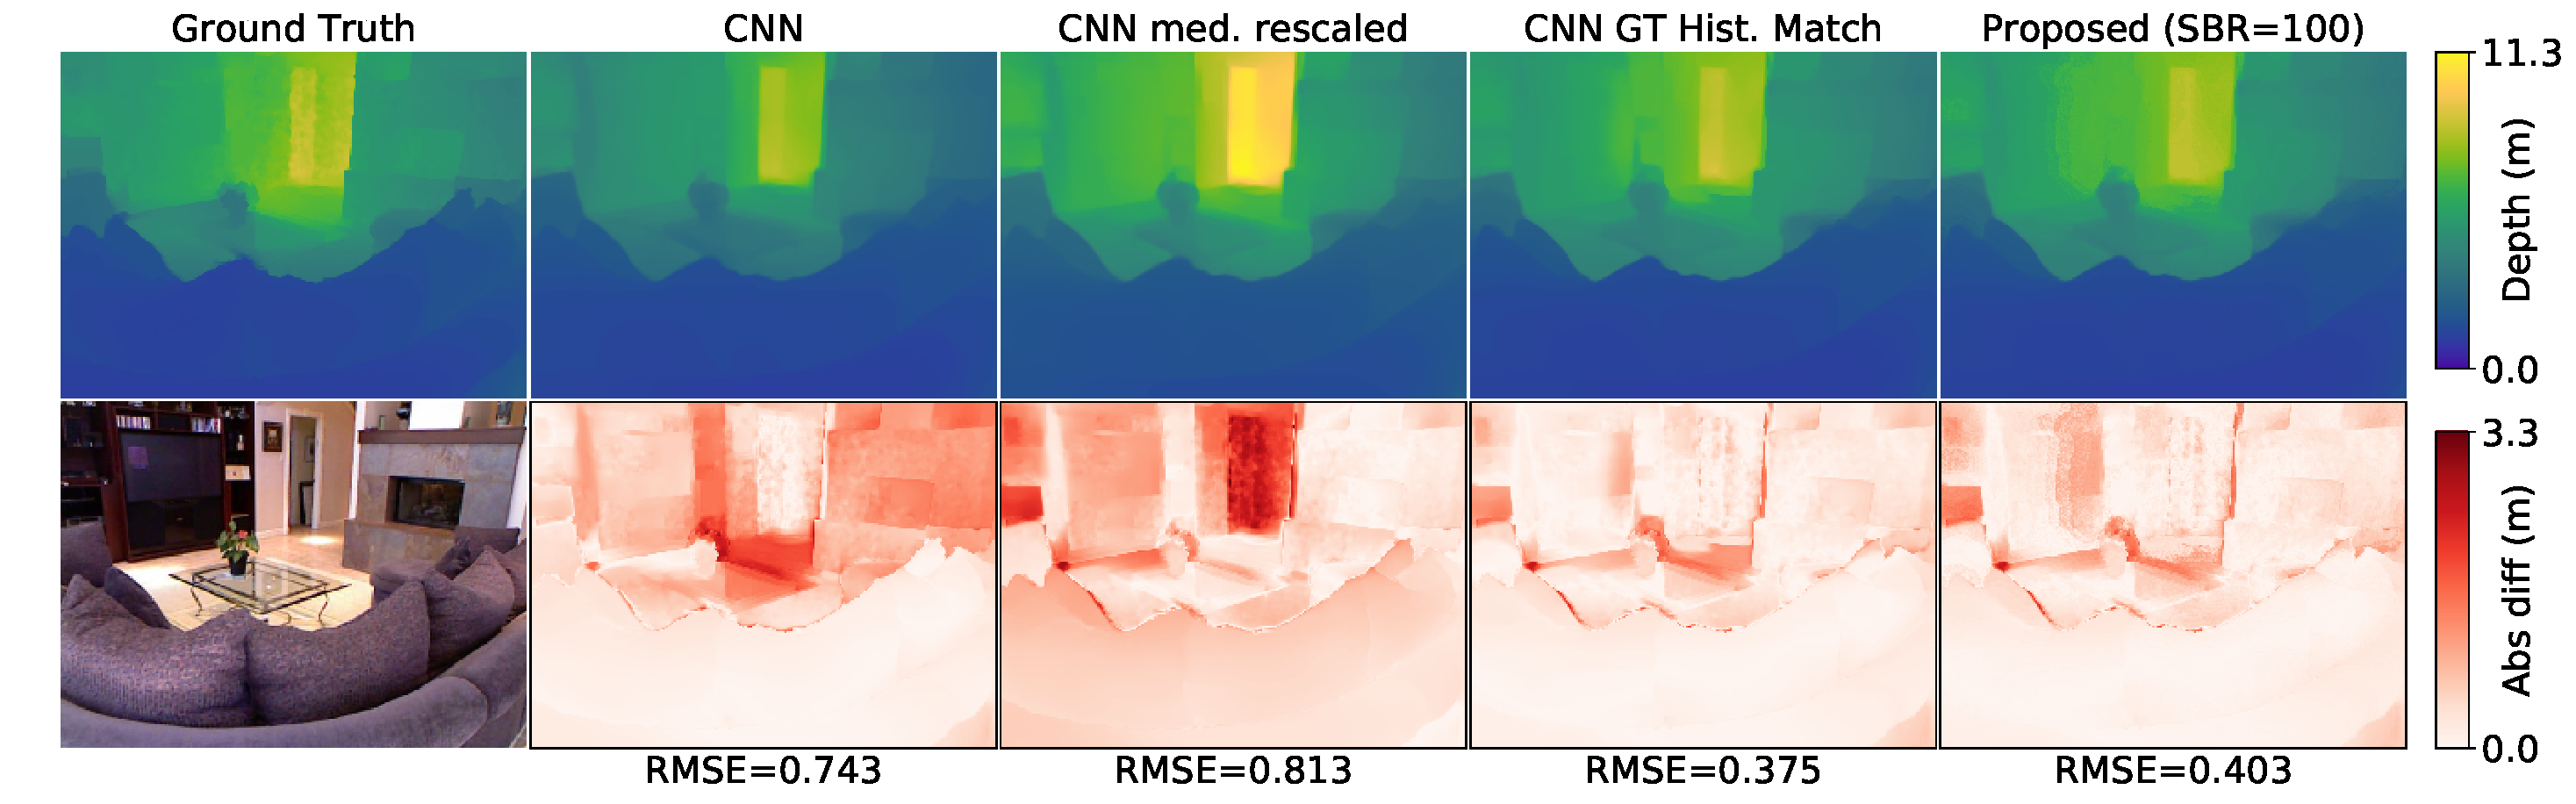
\includegraphics[width=\textwidth]{sections/figures/comparison/densedepth_529_comparison.png}
  \caption{Results on DenseDepth}
\end{figure*}
\begin{figure*}
  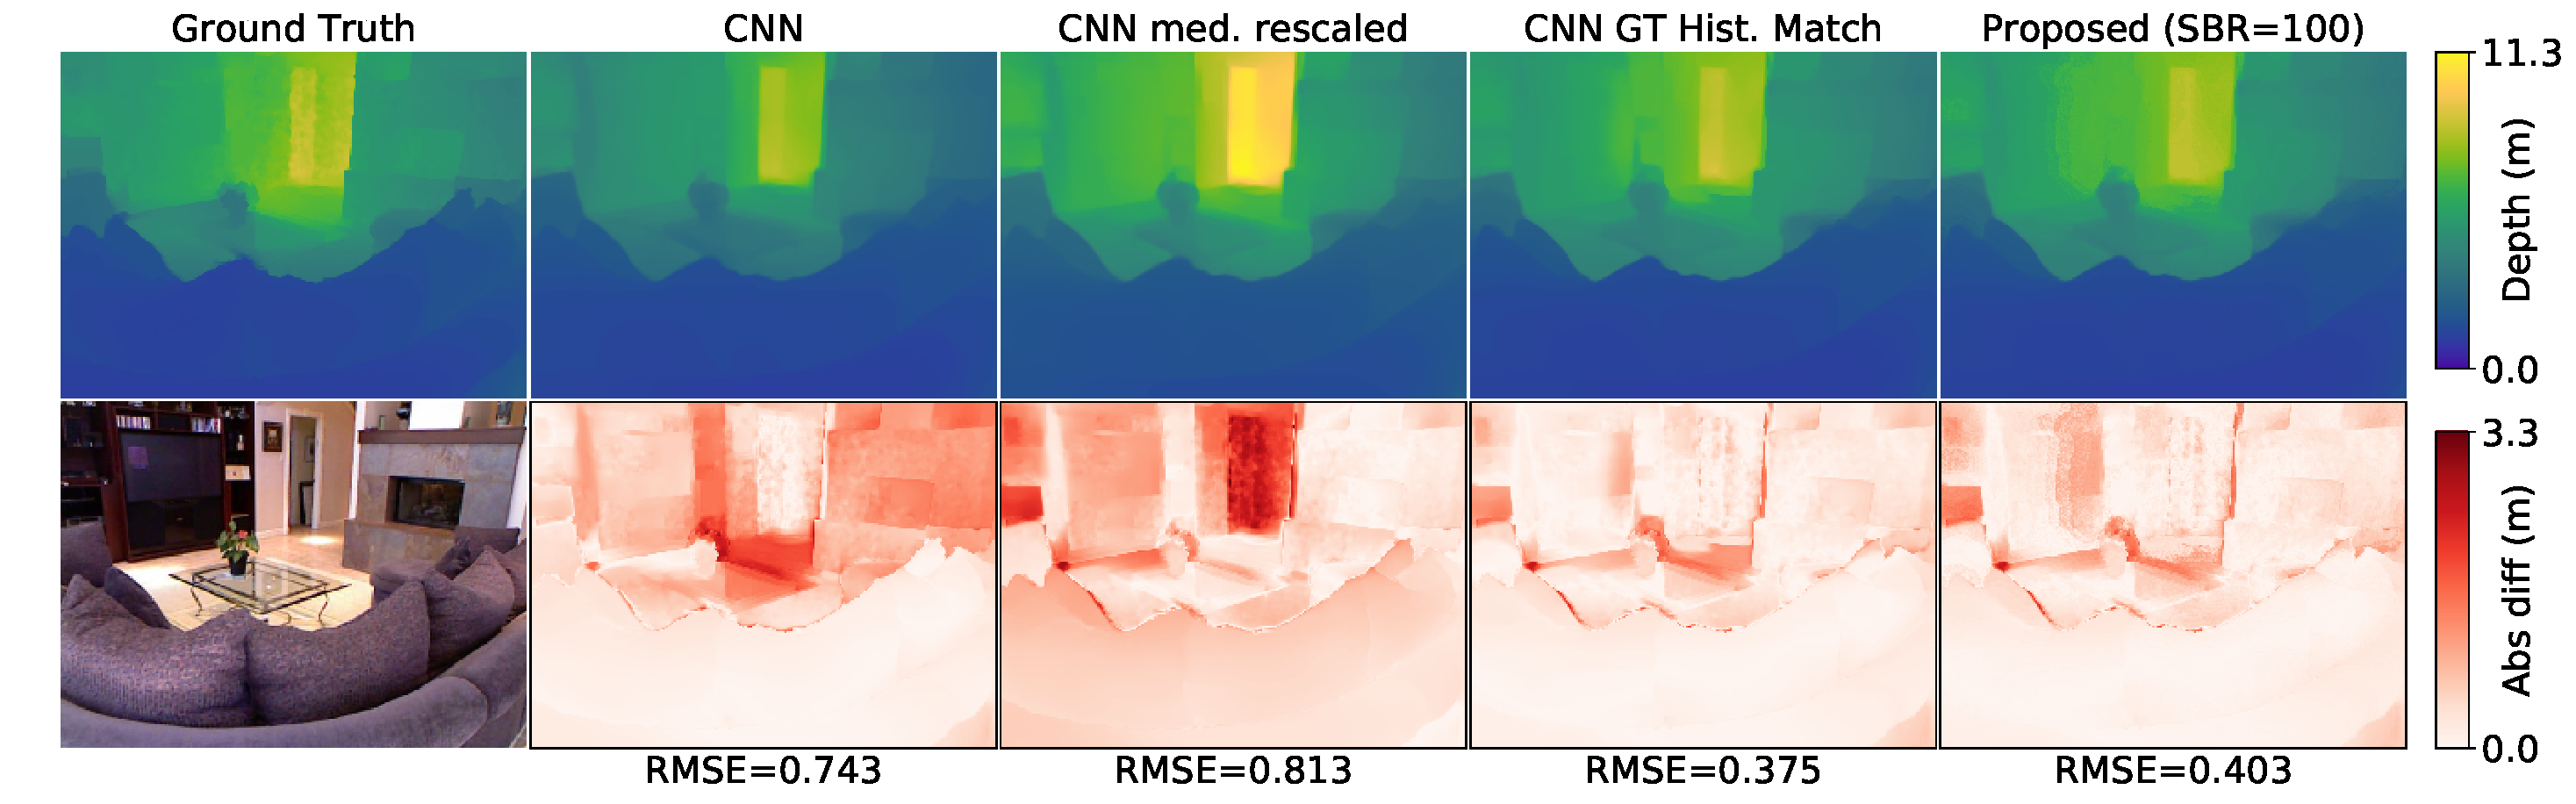
\includegraphics[width=\textwidth]{sections/figures/comparison/densedepth_529_comparison.png}
  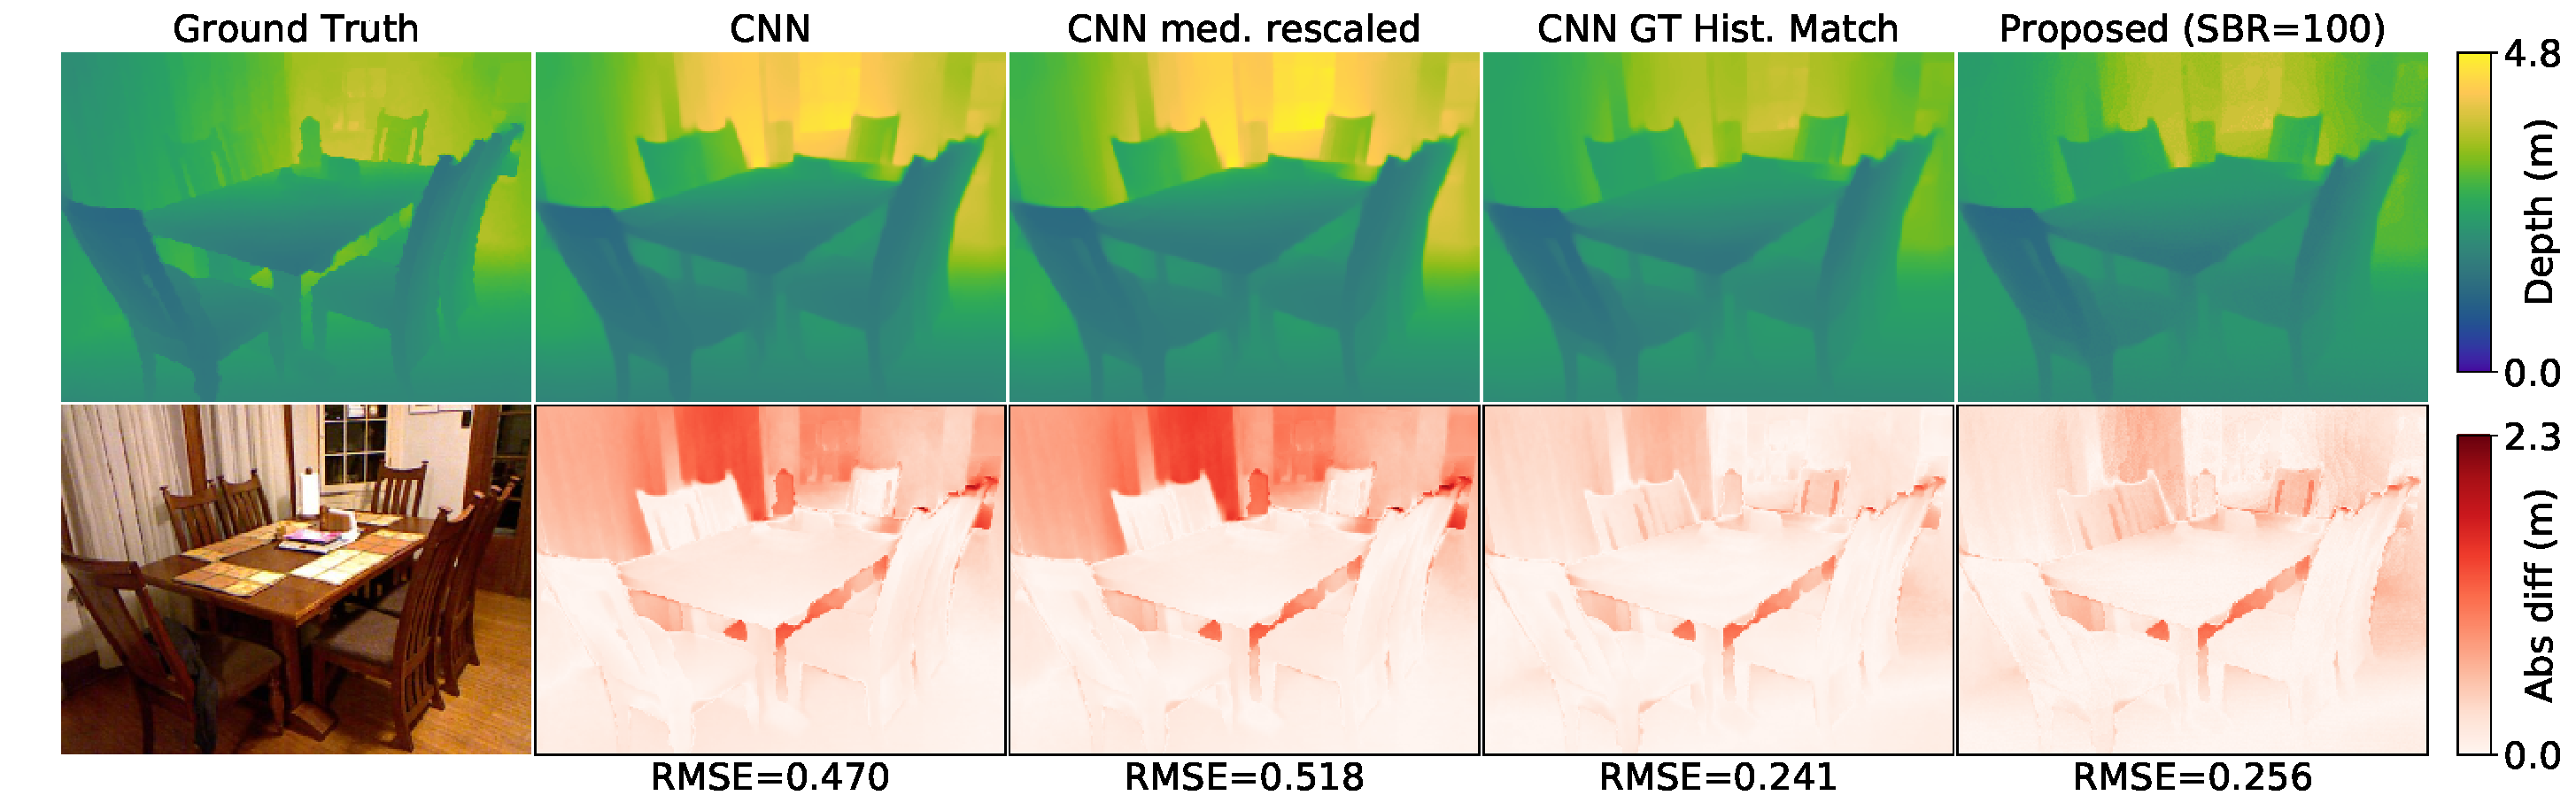
\includegraphics[width=\textwidth]{sections/figures/comparison/densedepth_219_comparison.png}
  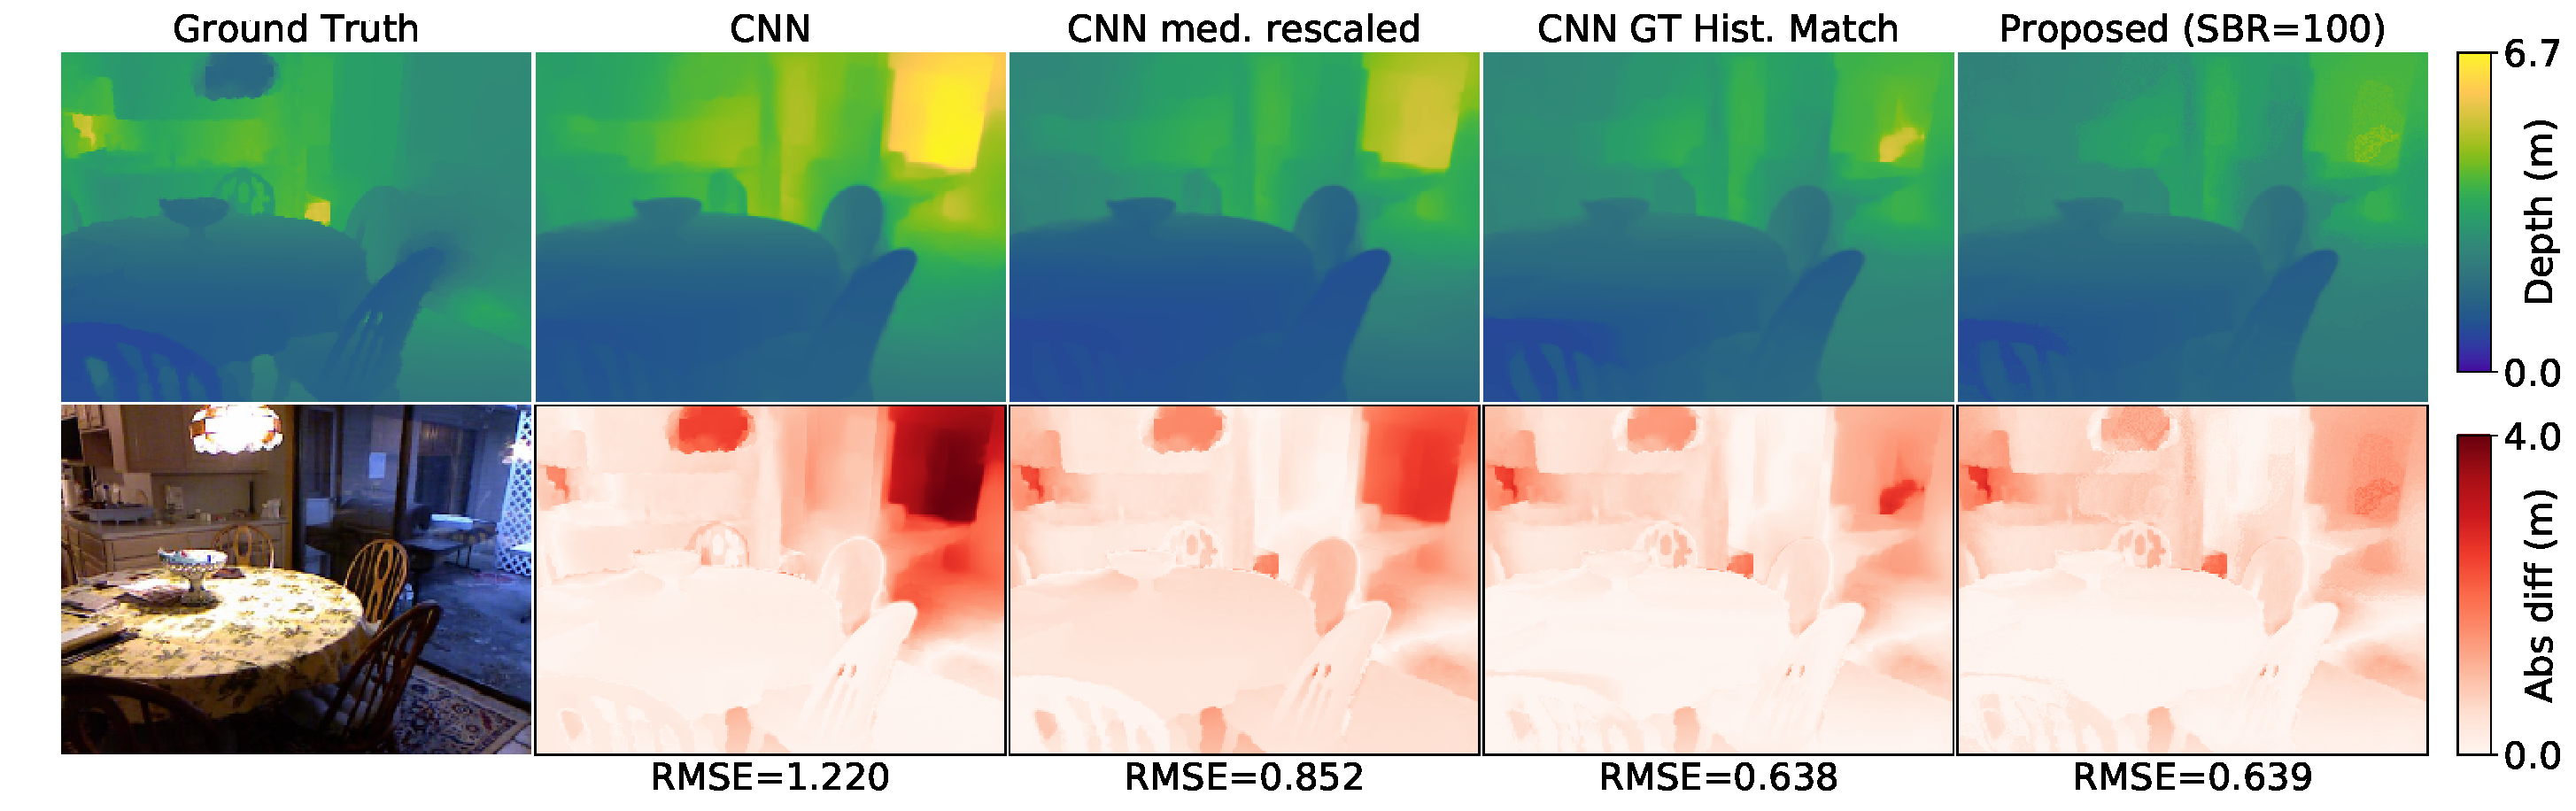
\includegraphics[width=\textwidth]{sections/figures/comparison/densedepth_329_comparison.png}
  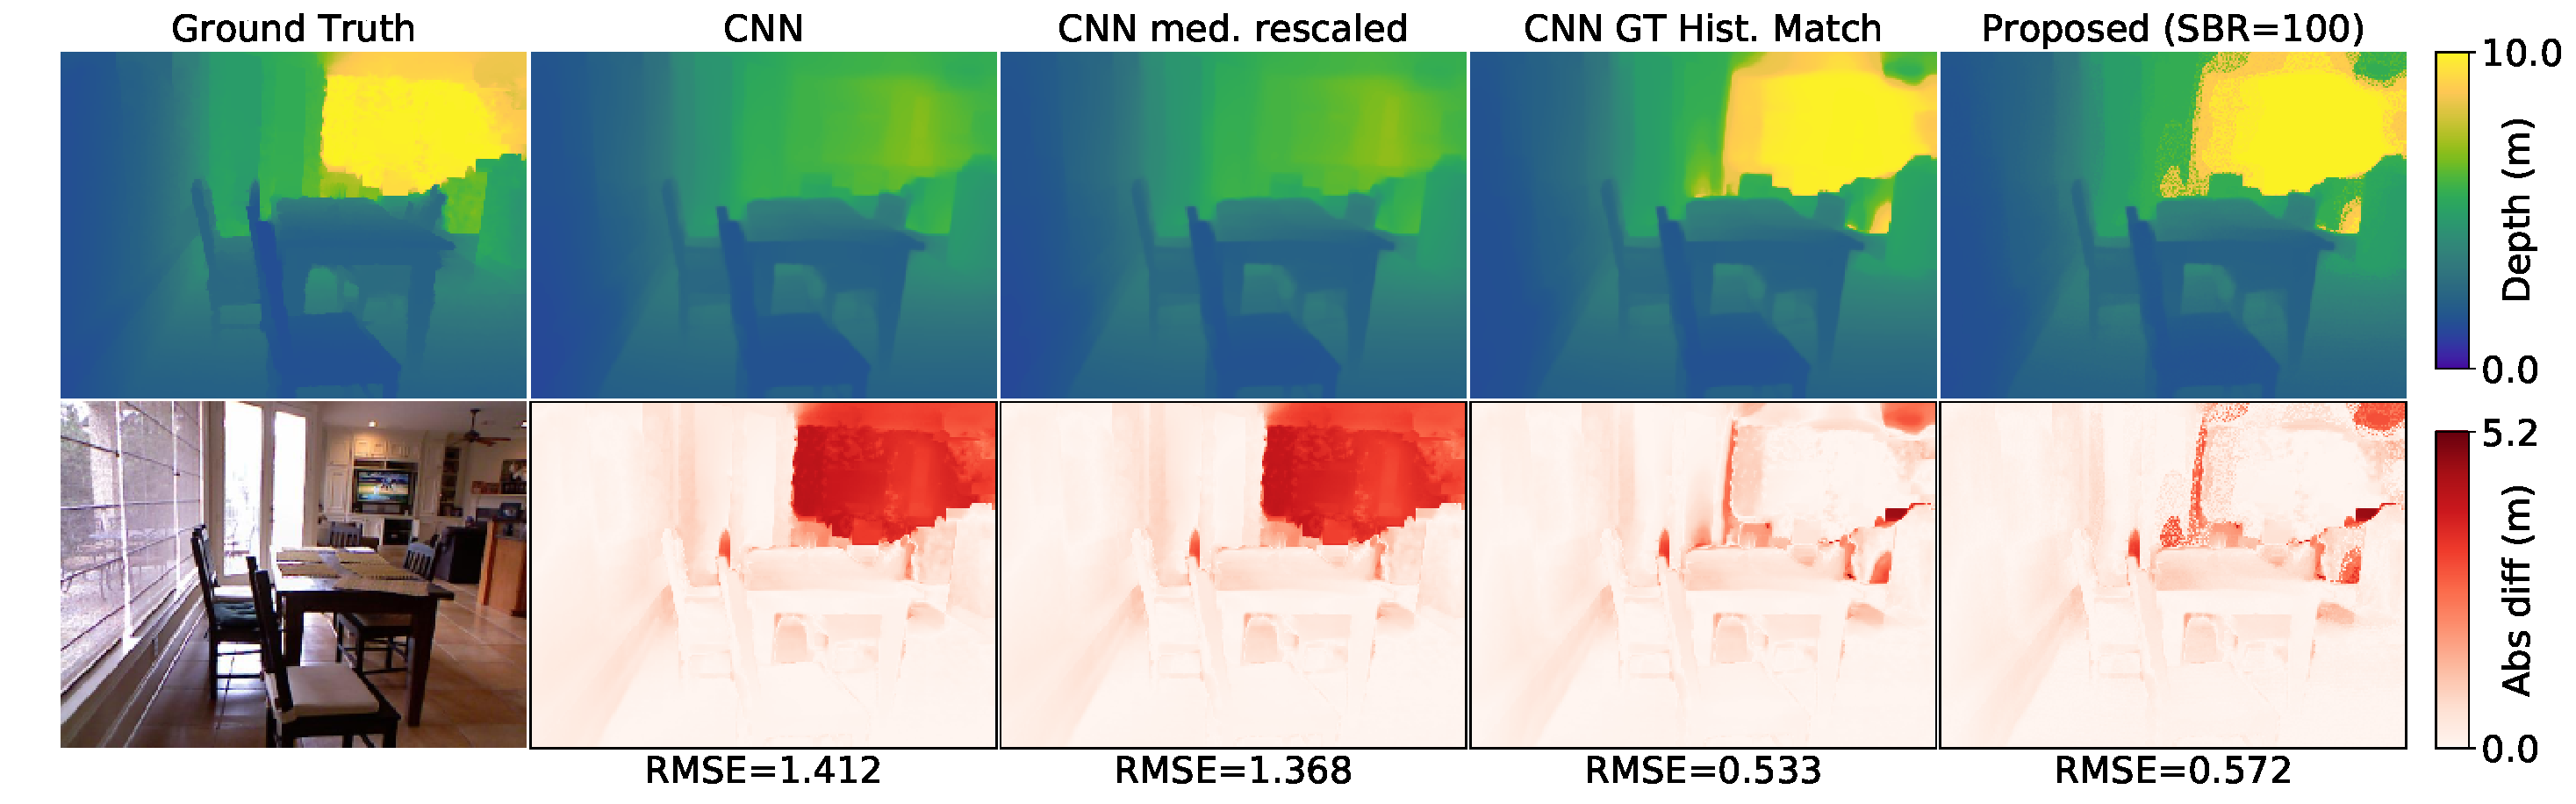
\includegraphics[width=\textwidth]{sections/figures/comparison/densedepth_346_comparison.png}
  \caption{Results on DenseDepth}
\end{figure*}
\begin{figure*}
  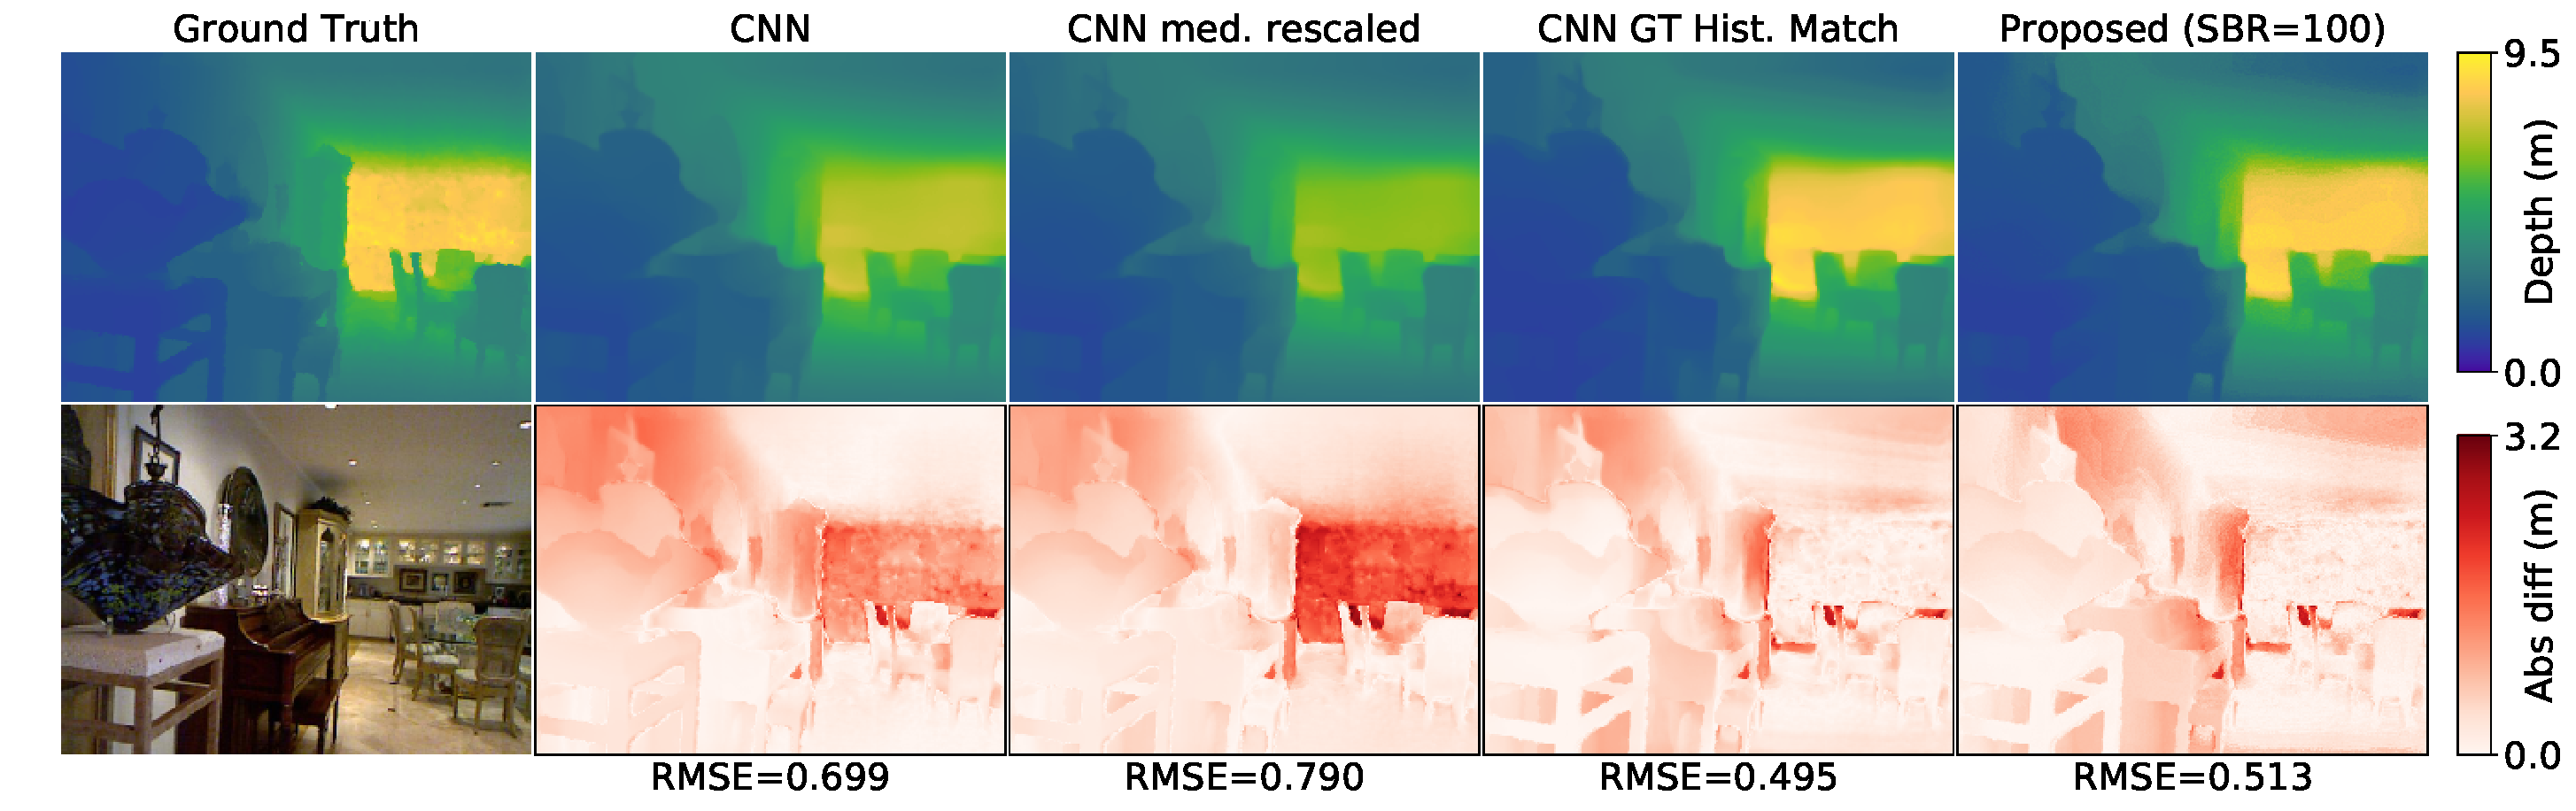
\includegraphics[width=\textwidth]{sections/figures/comparison/densedepth_616_comparison.png}
  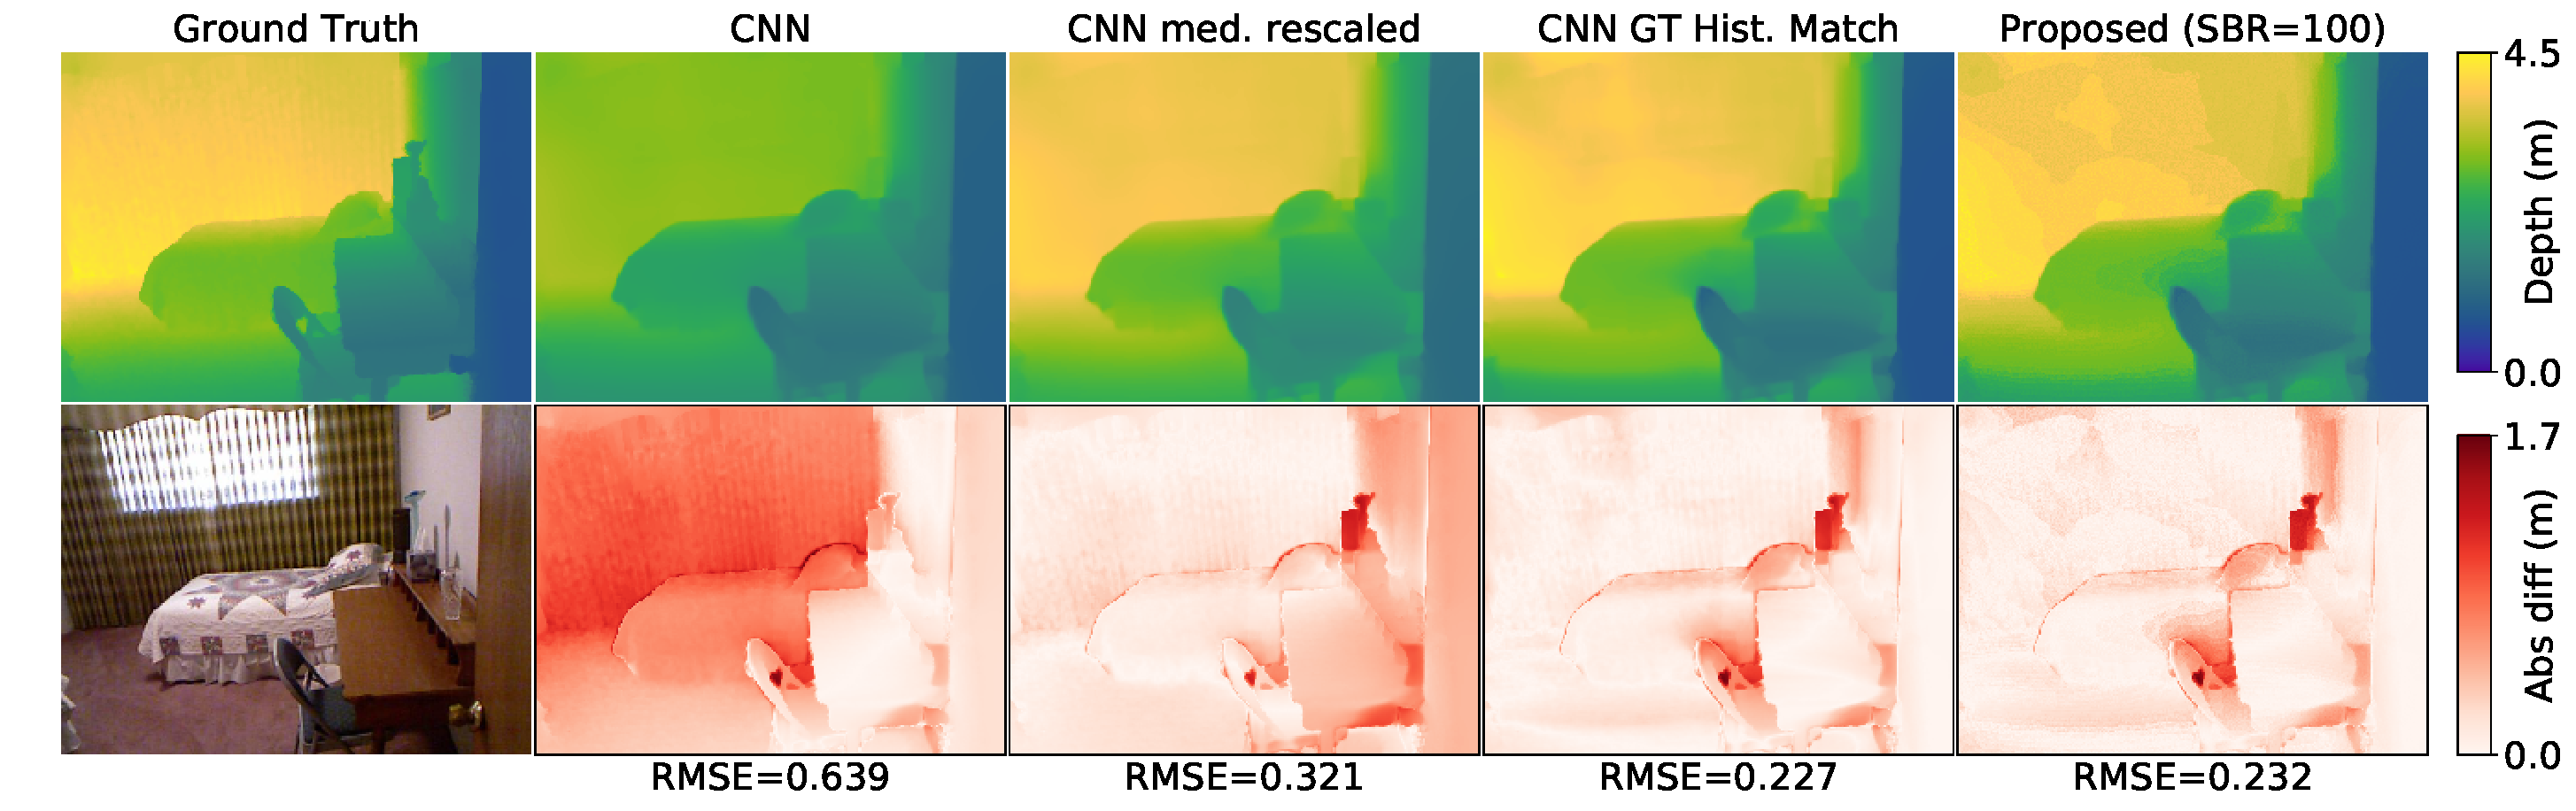
\includegraphics[width=\textwidth]{sections/figures/comparison/densedepth_390_comparison.png}
  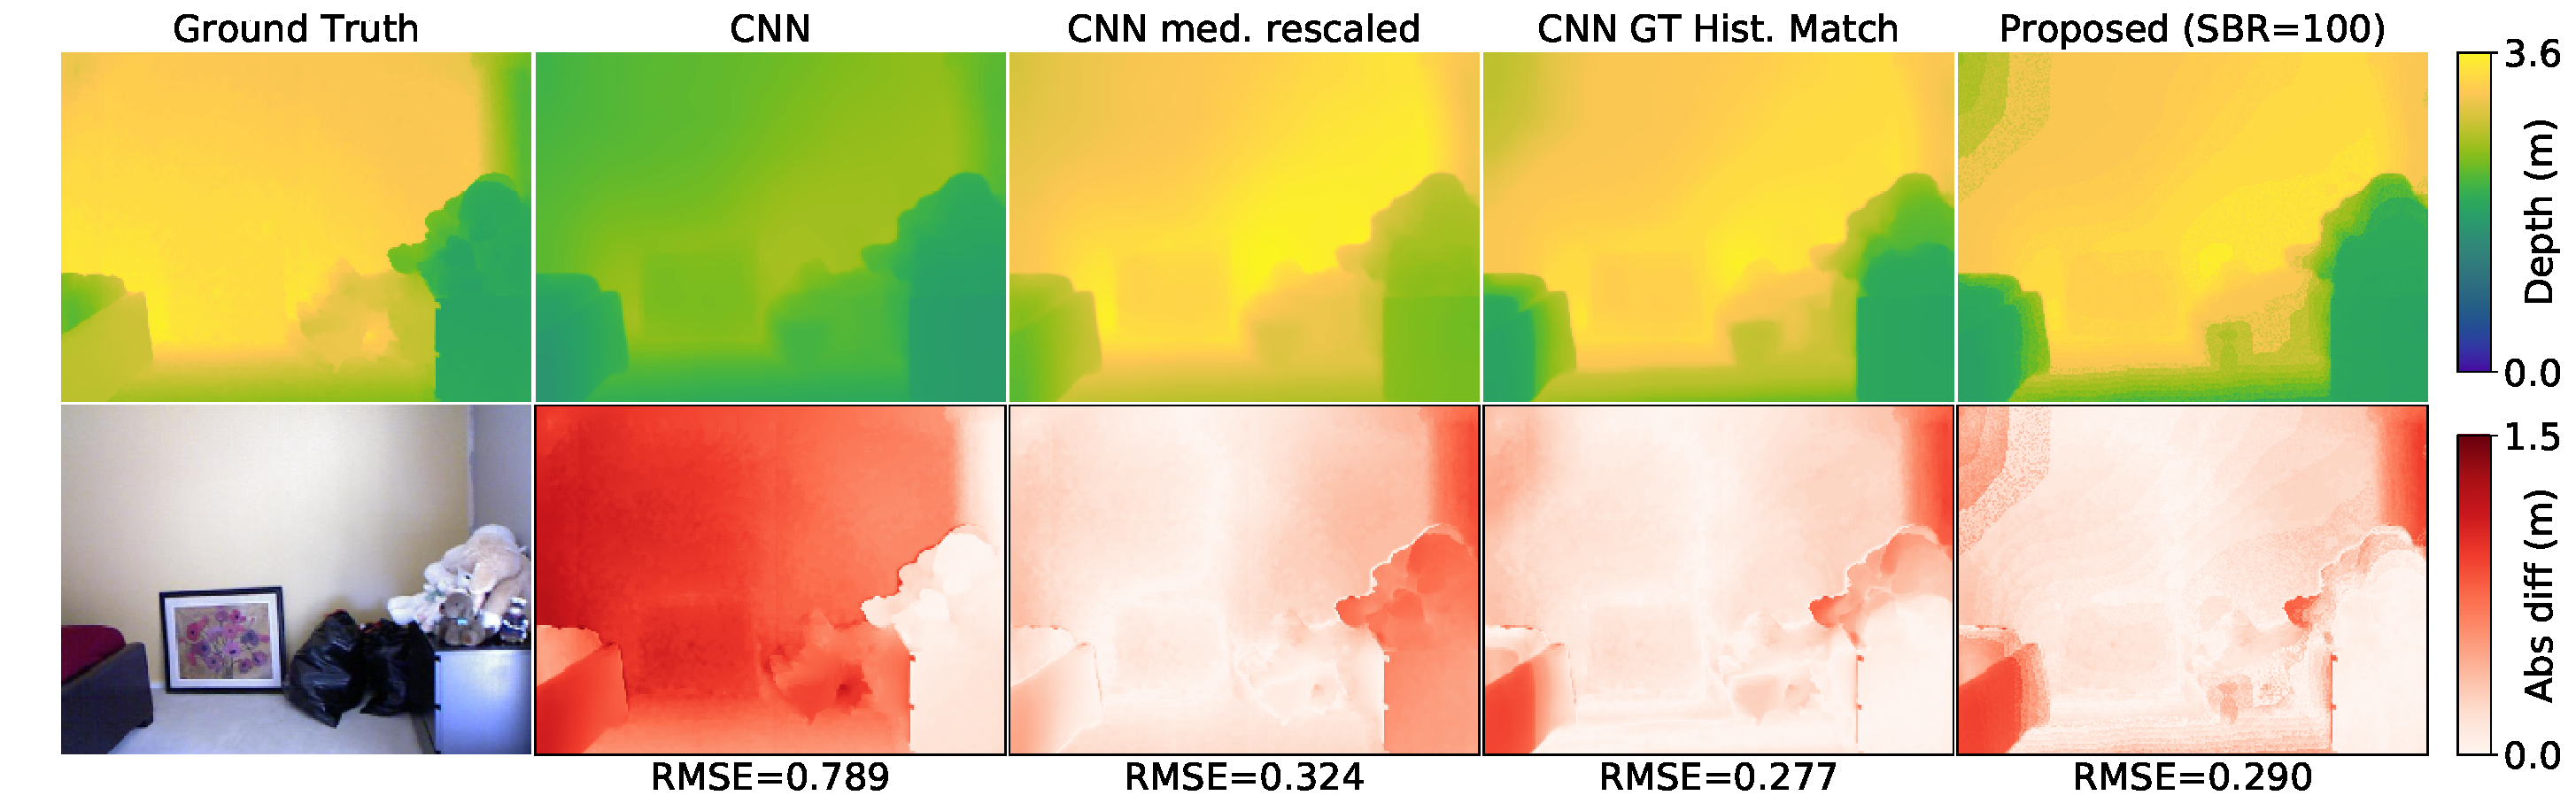
\includegraphics[width=\textwidth]{sections/figures/comparison/densedepth_412_comparison.png}
  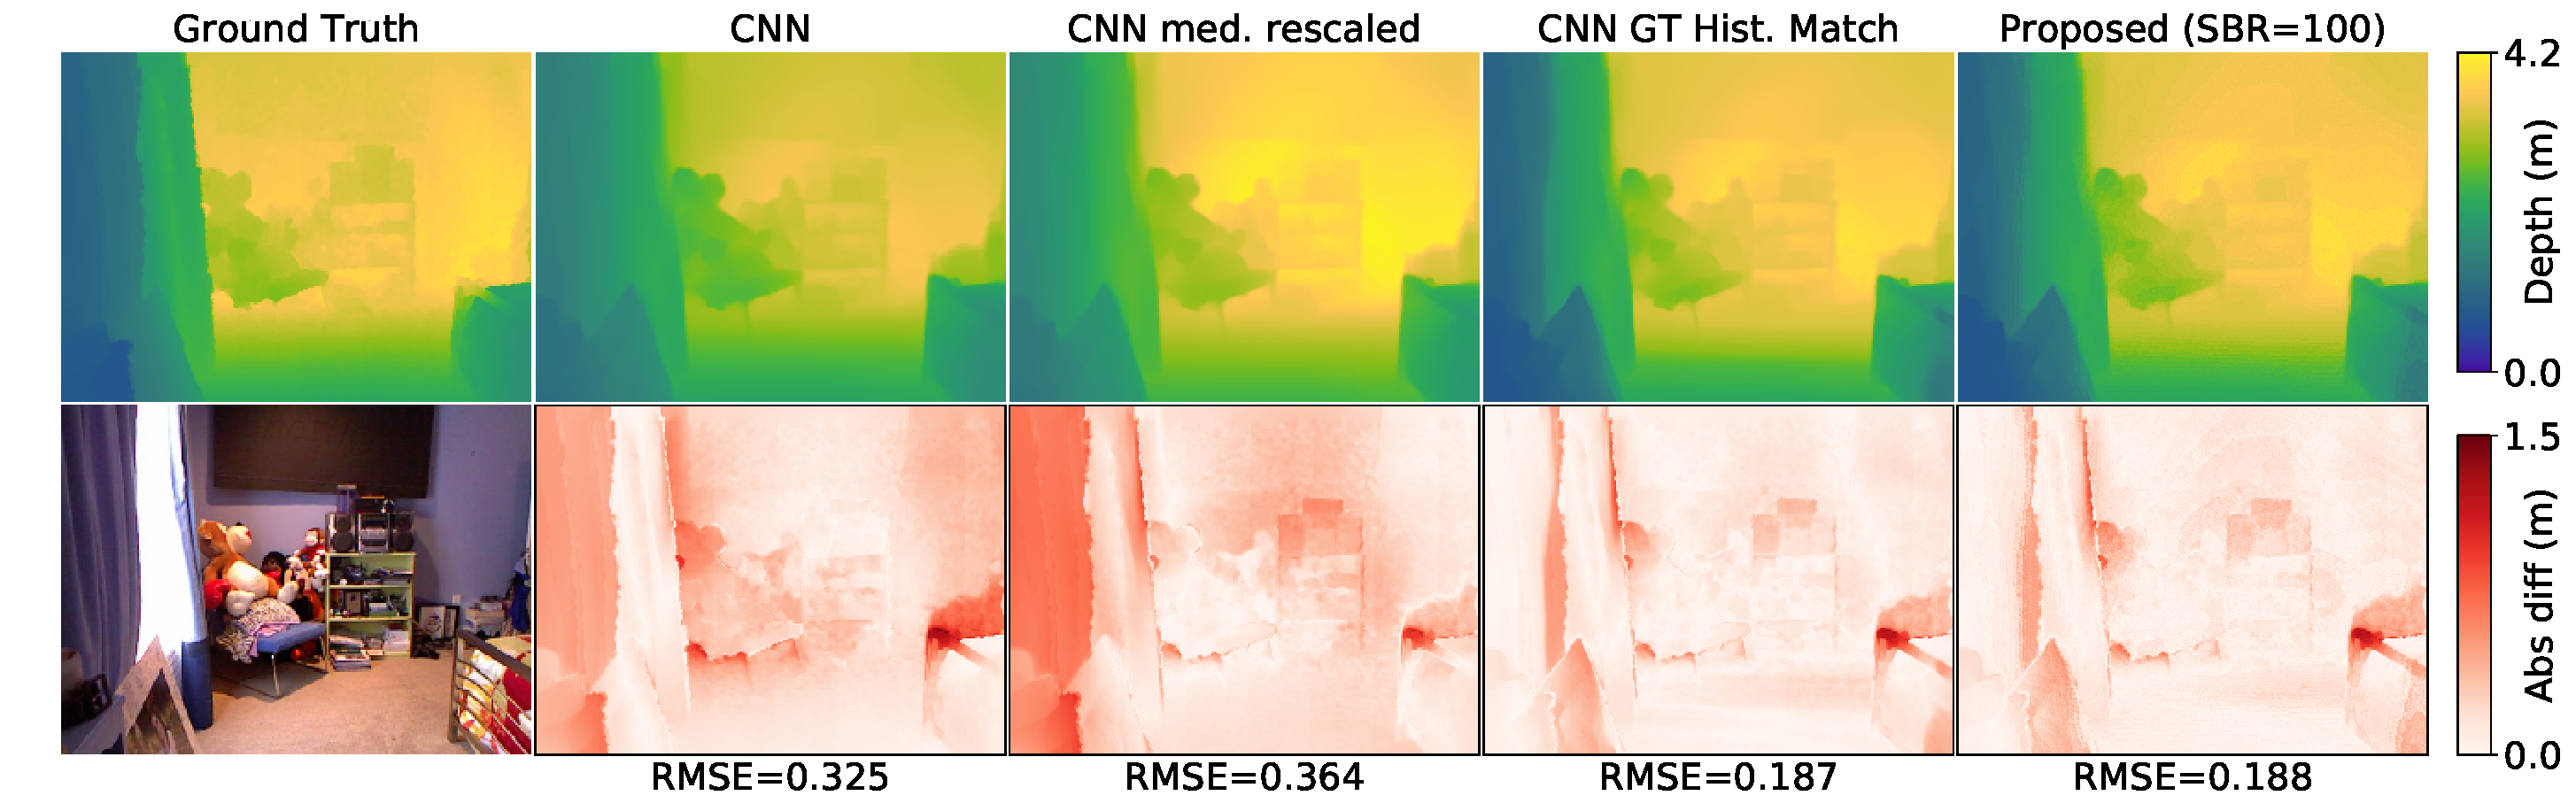
\includegraphics[width=\textwidth]{sections/figures/comparison/densedepth_420_comparison.png}
  \caption{Results on DenseDepth}
\end{figure*}
\begin{figure*}
  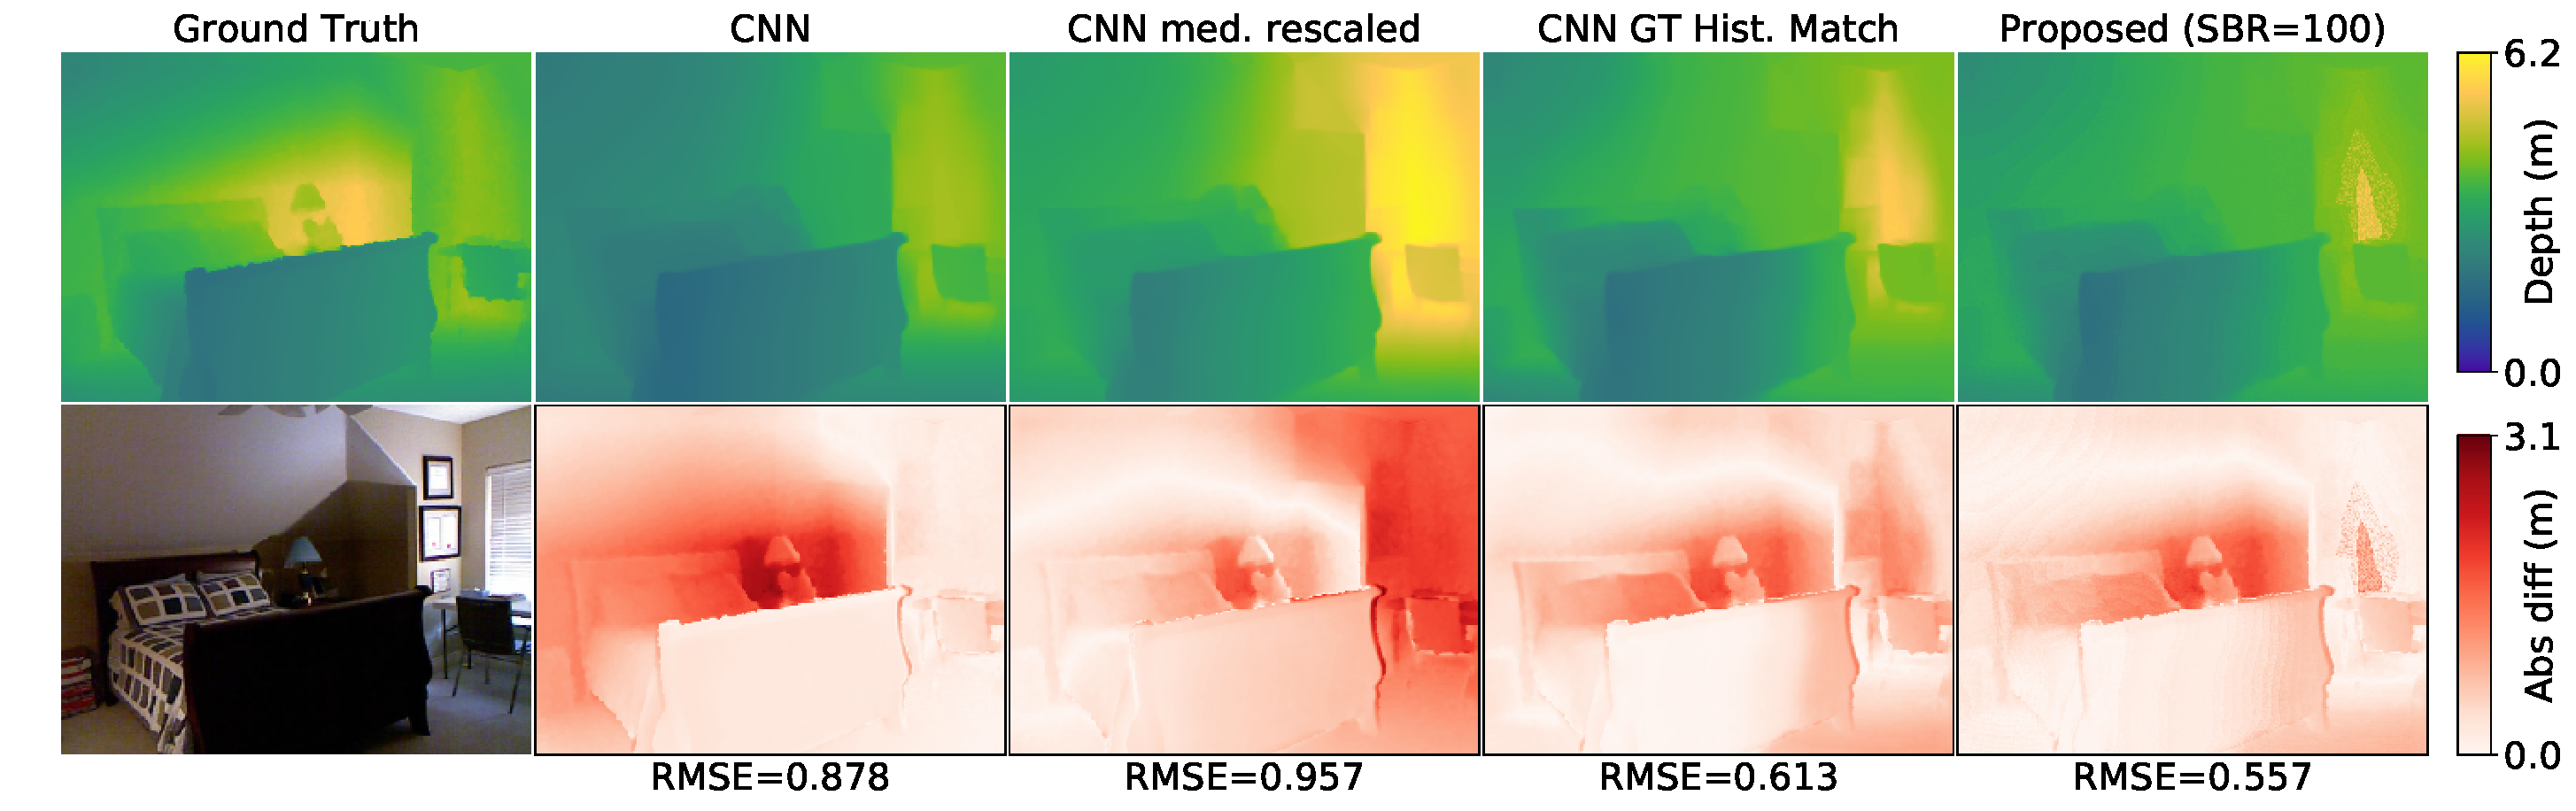
\includegraphics[width=\textwidth]{sections/figures/comparison/densedepth_428_comparison.png}
  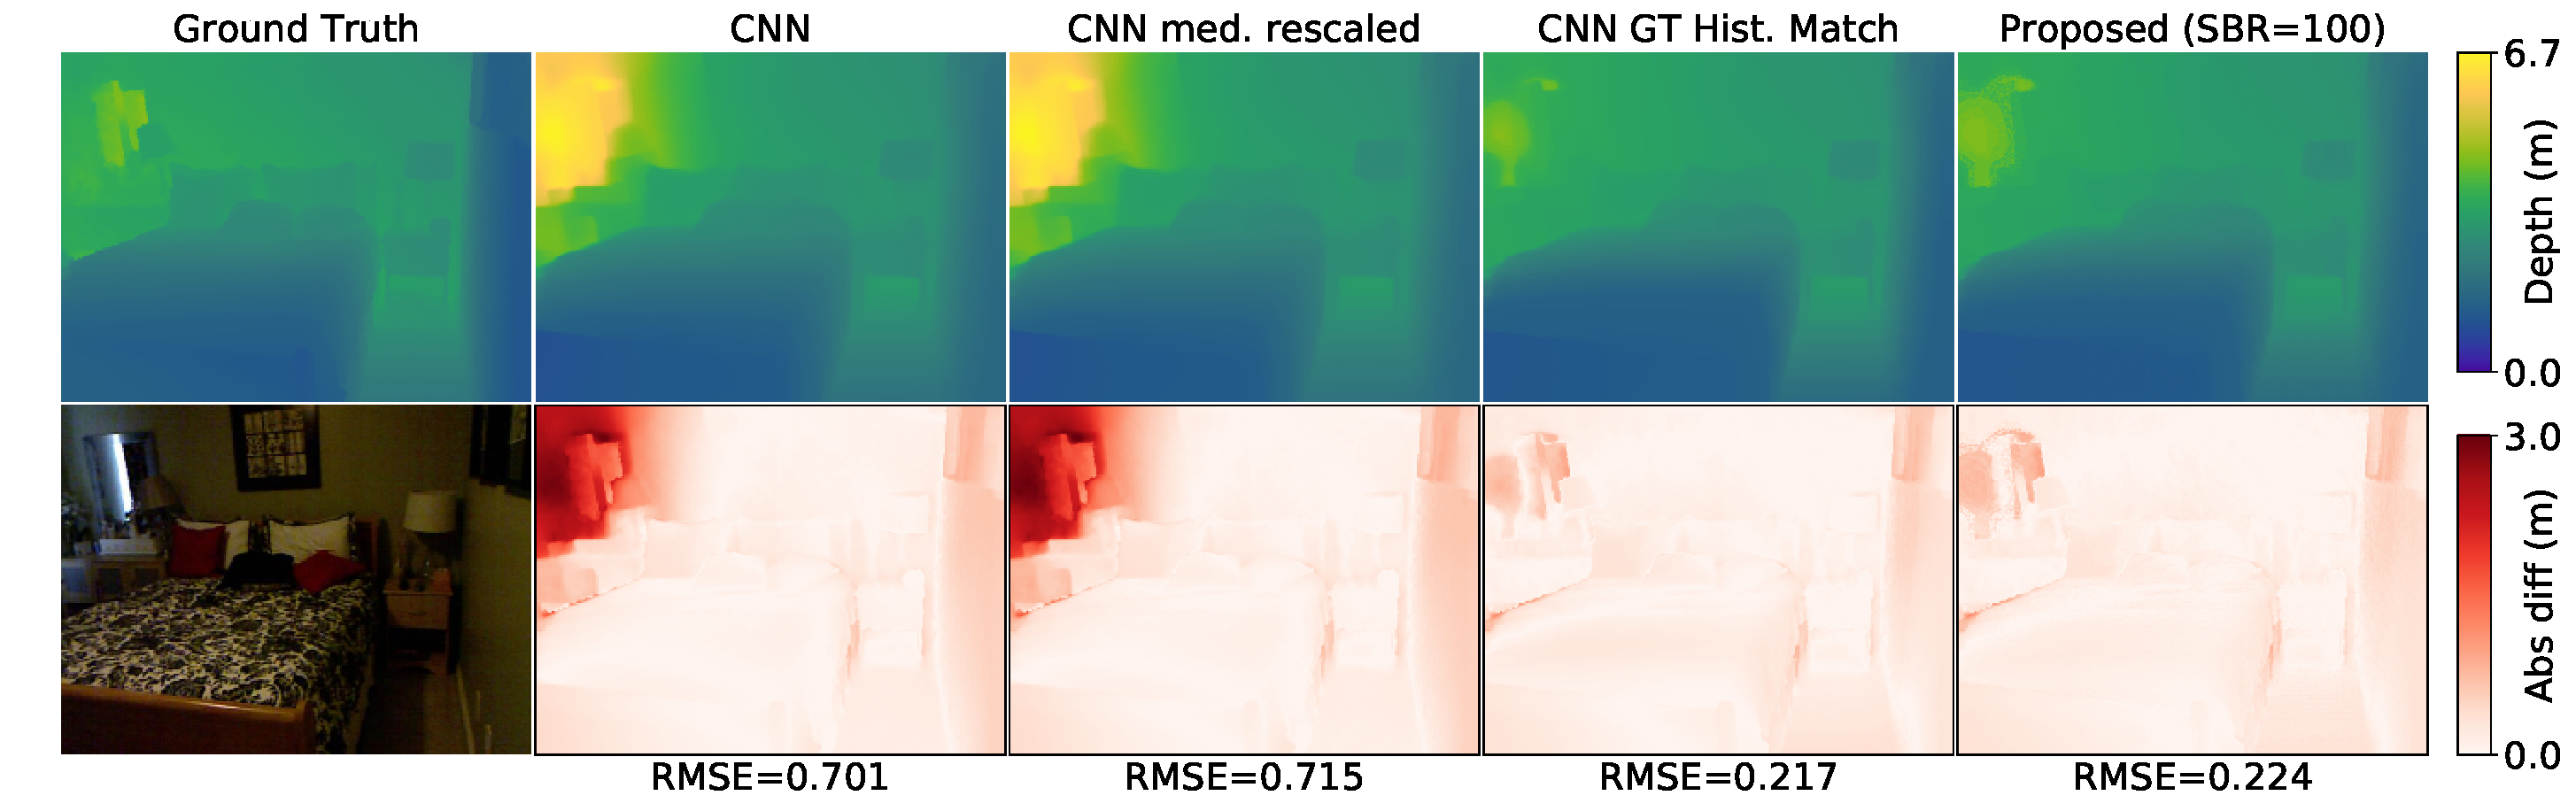
\includegraphics[width=\textwidth]{sections/figures/comparison/densedepth_457_comparison.png}
  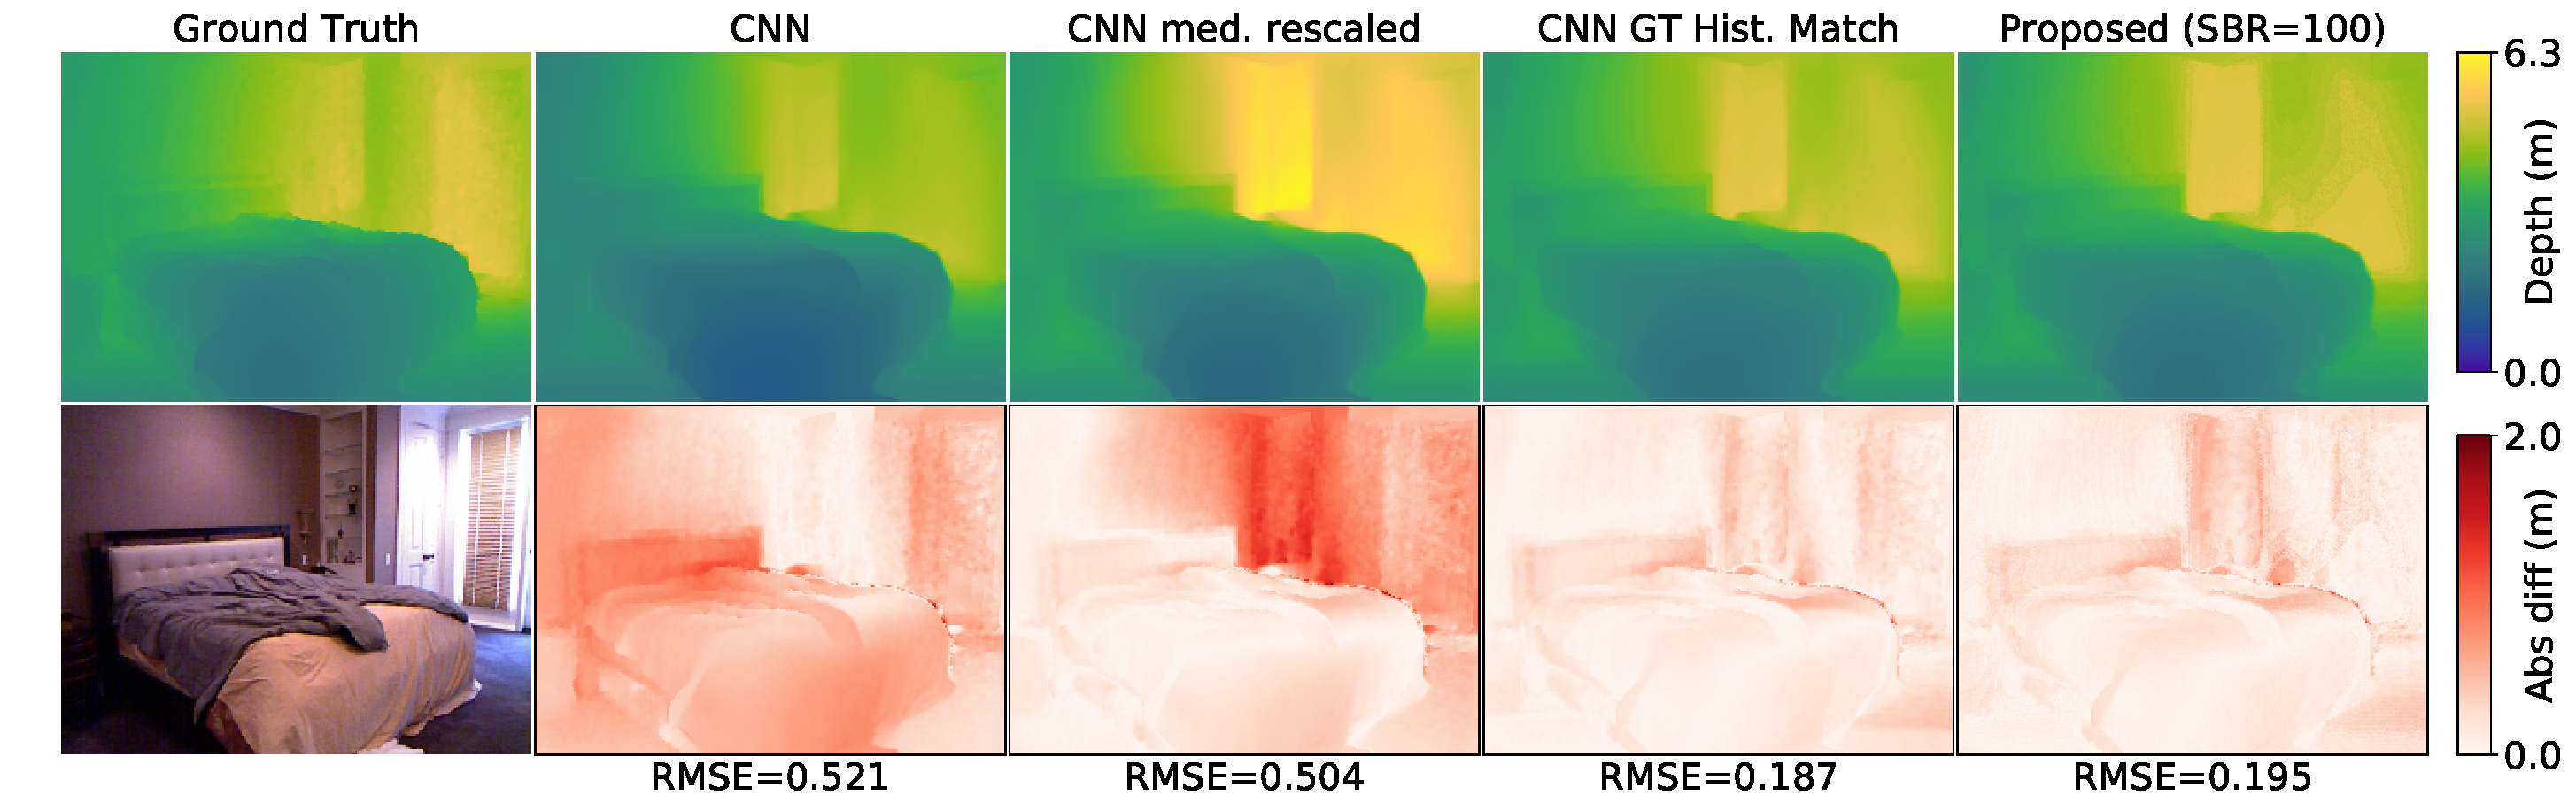
\includegraphics[width=\textwidth]{sections/figures/comparison/densedepth_468_comparison.png}
  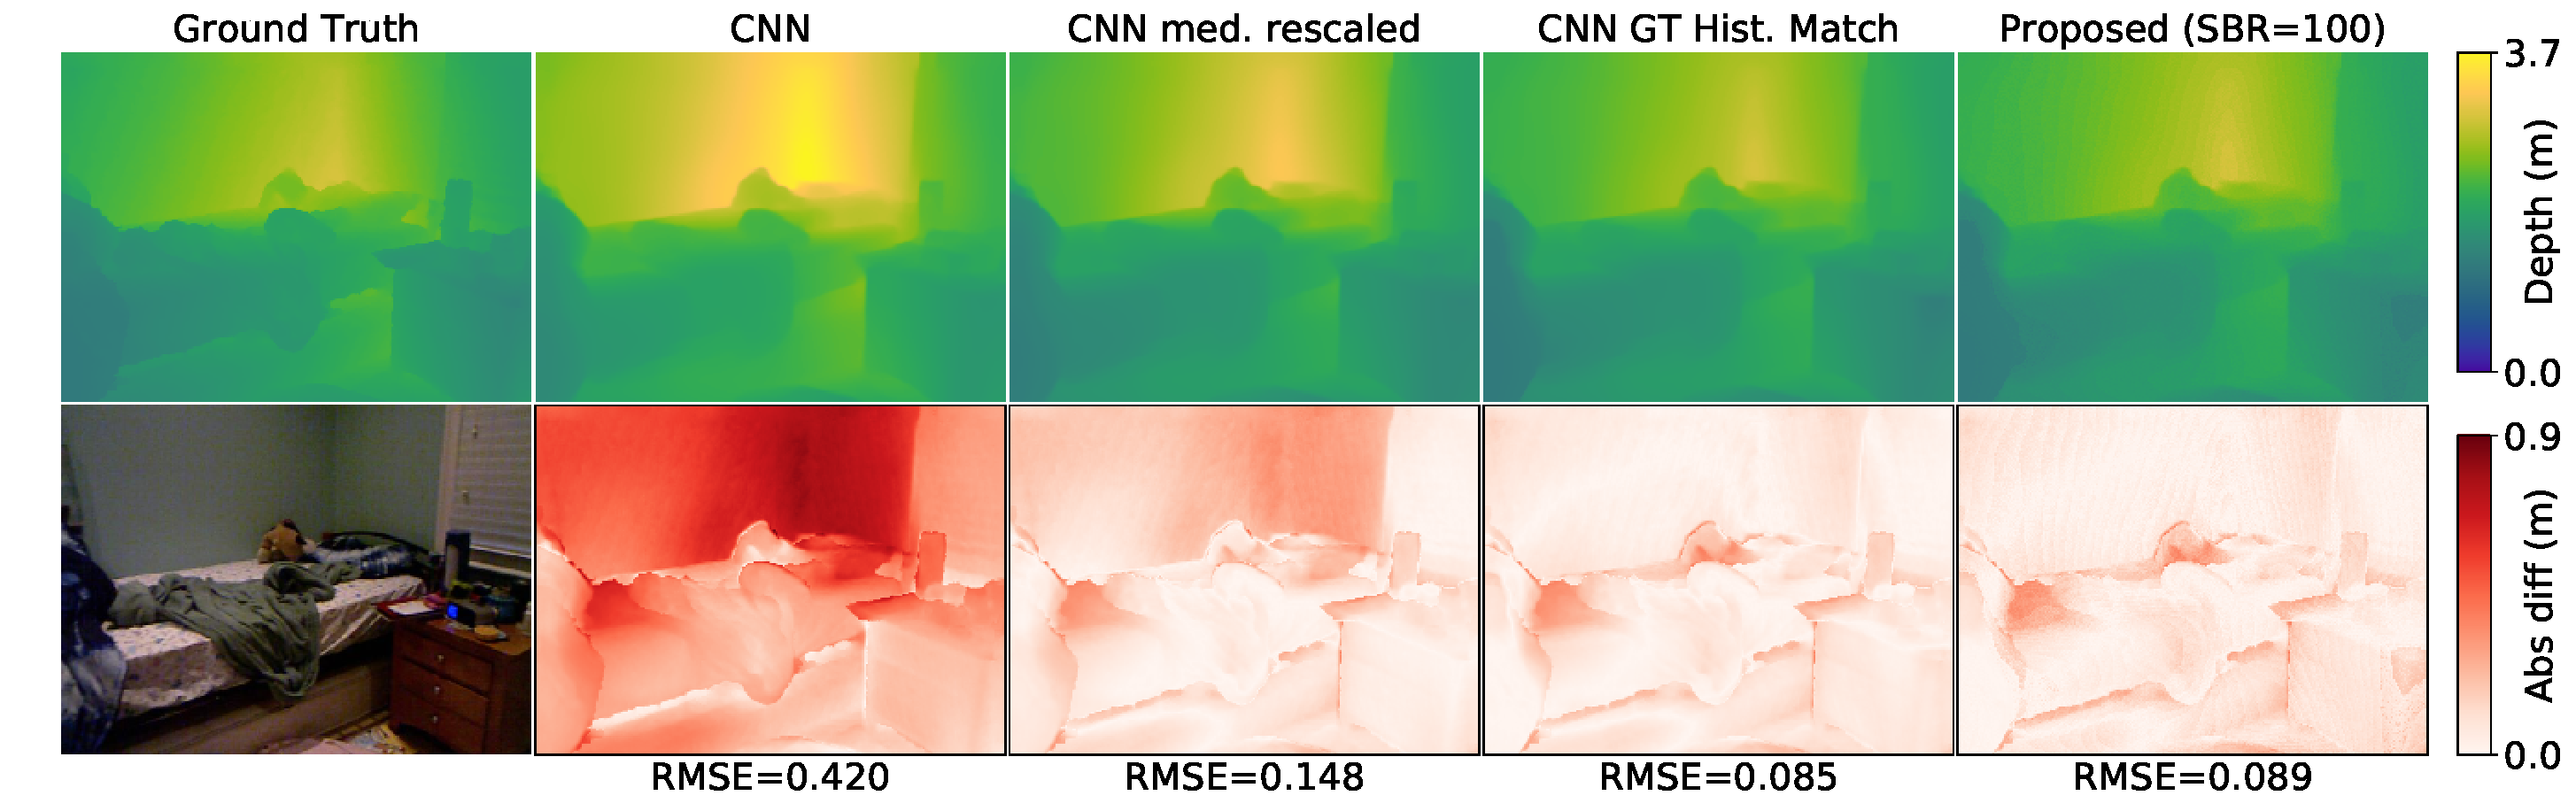
\includegraphics[width=\textwidth]{sections/figures/comparison/densedepth_477_comparison.png}
  \caption{Results on DenseDepth}
\end{figure*}
%   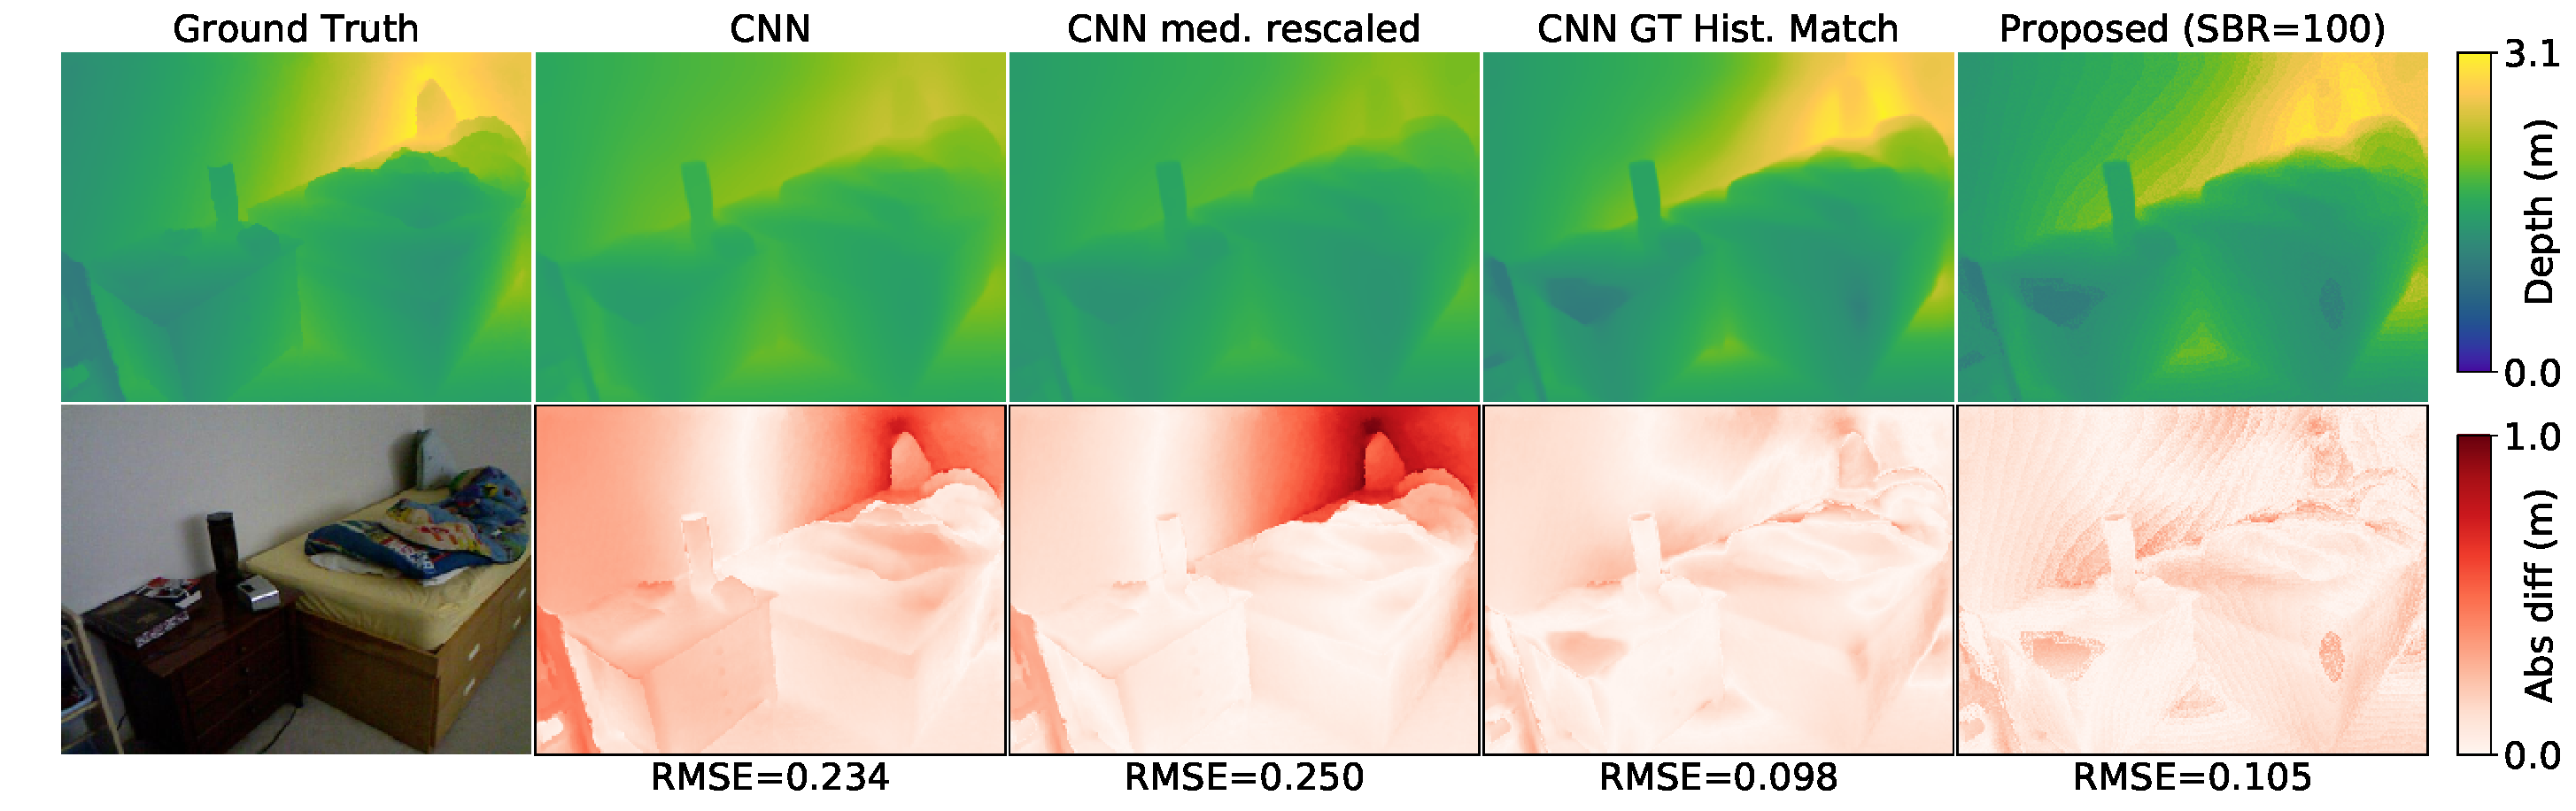
\includegraphics[height=3cm]{sections/figures/comparison/densedepth_499_comparison.png}
%   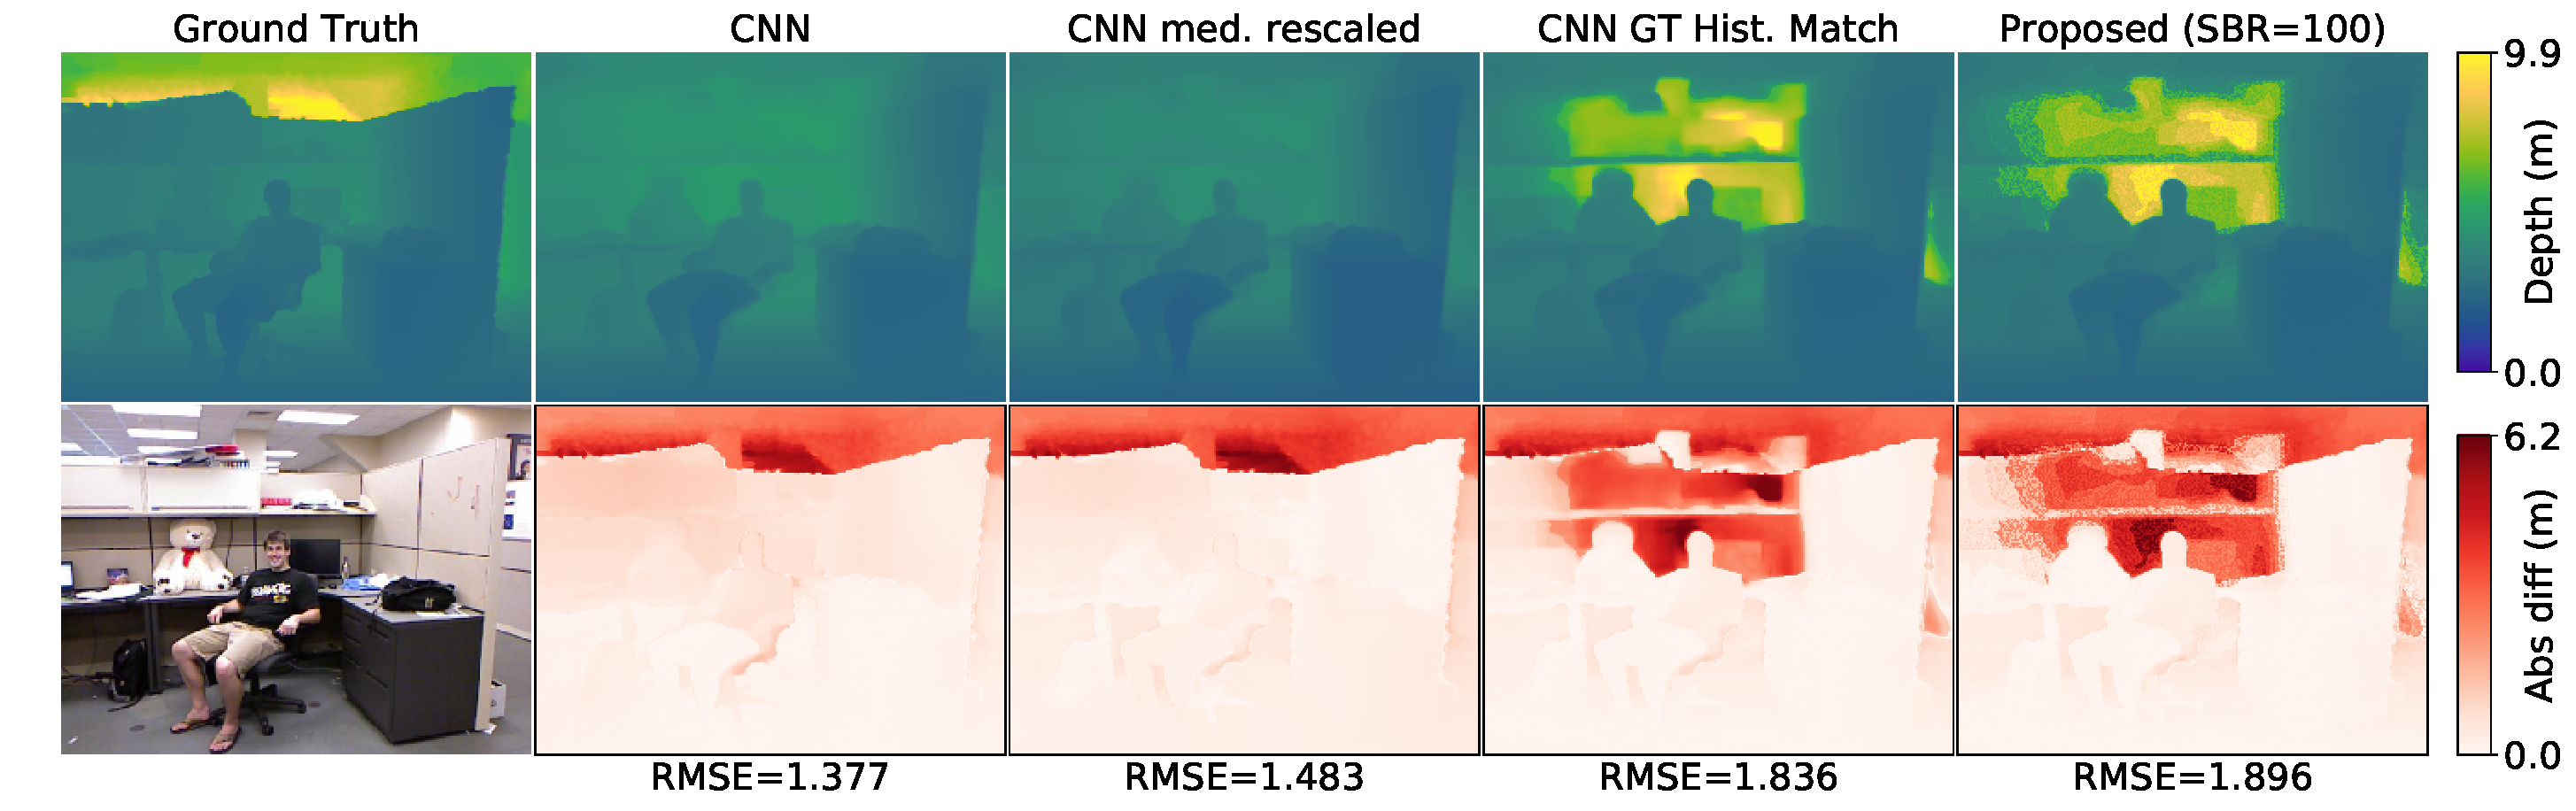
\includegraphics[height=3cm]{sections/figures/comparison/densedepth_258_comparison.png}
%   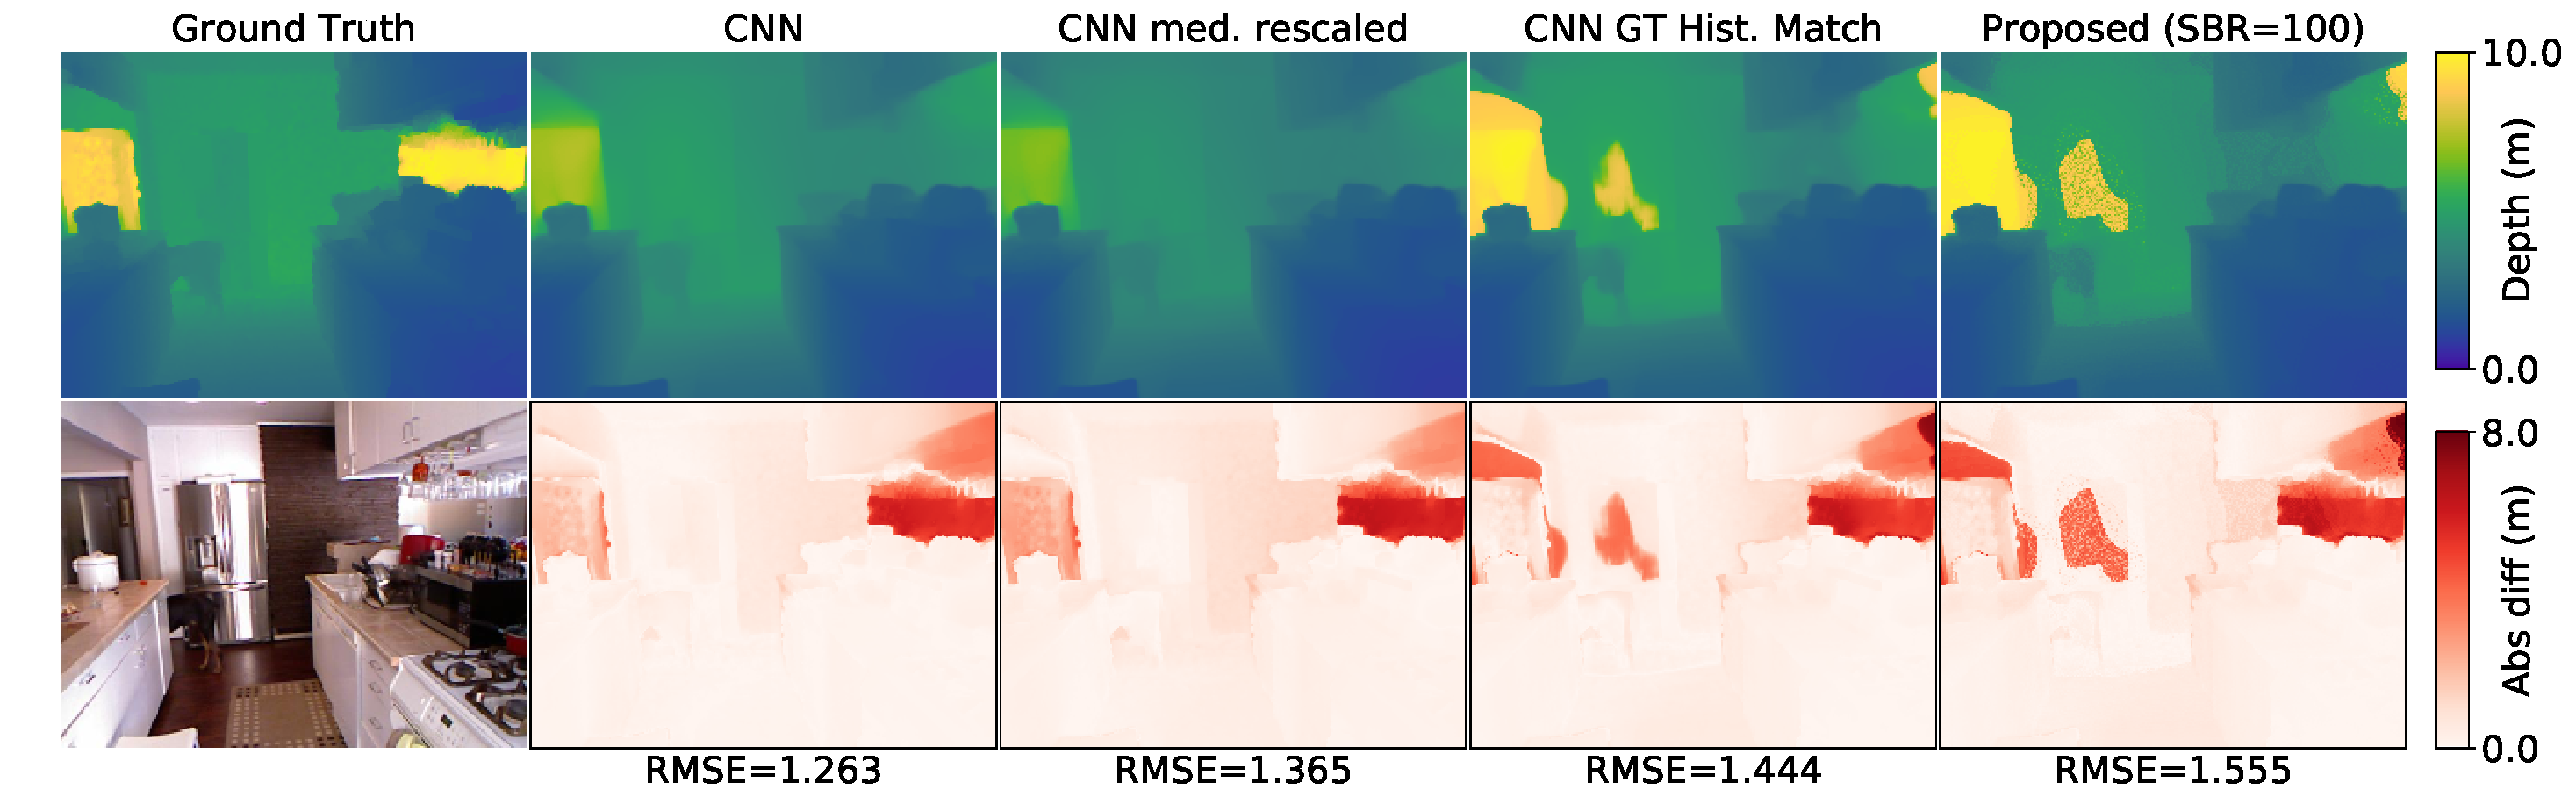
\includegraphics[height=3cm]{sections/figures/comparison/densedepth_341_comparison.png}
<<<<<<< HEAD

=======
\begin{figure*}
  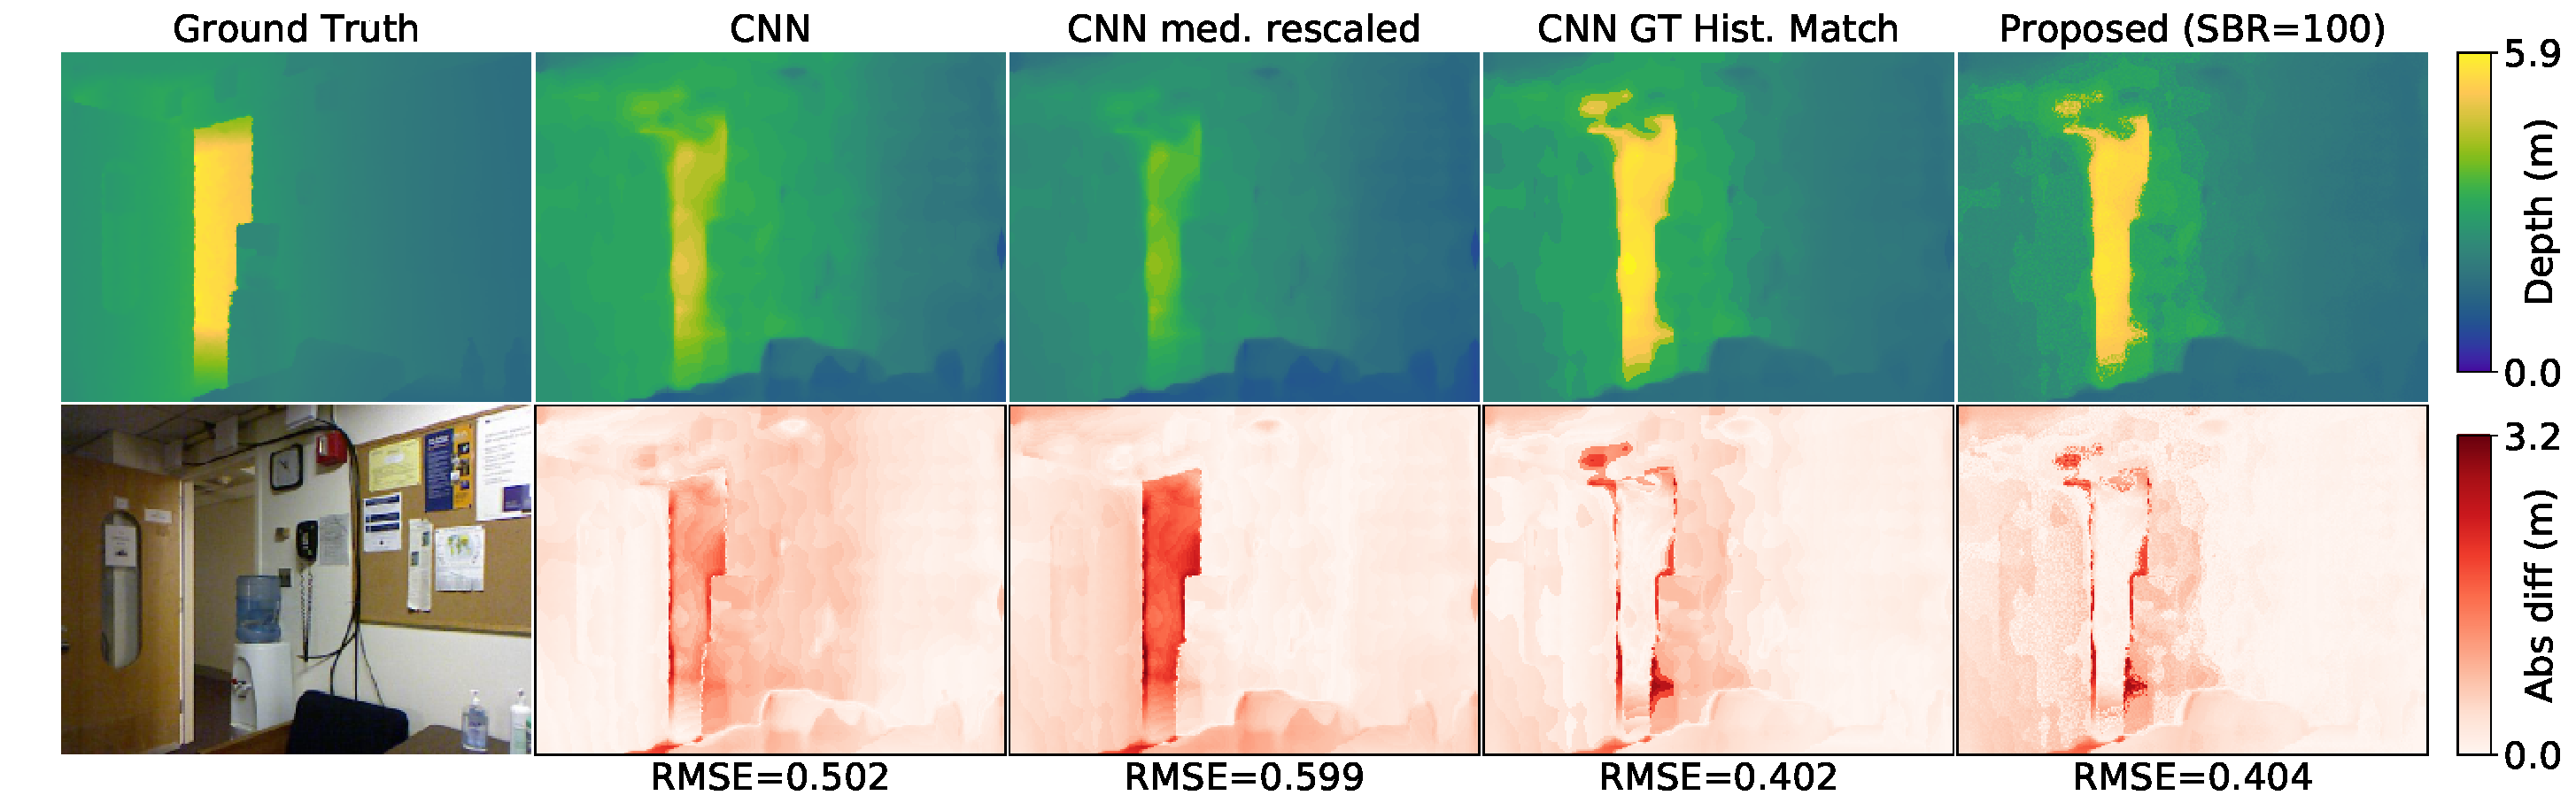
\includegraphics[width=\textwidth]{sections/figures/comparison/dorn_8_comparison.png}
  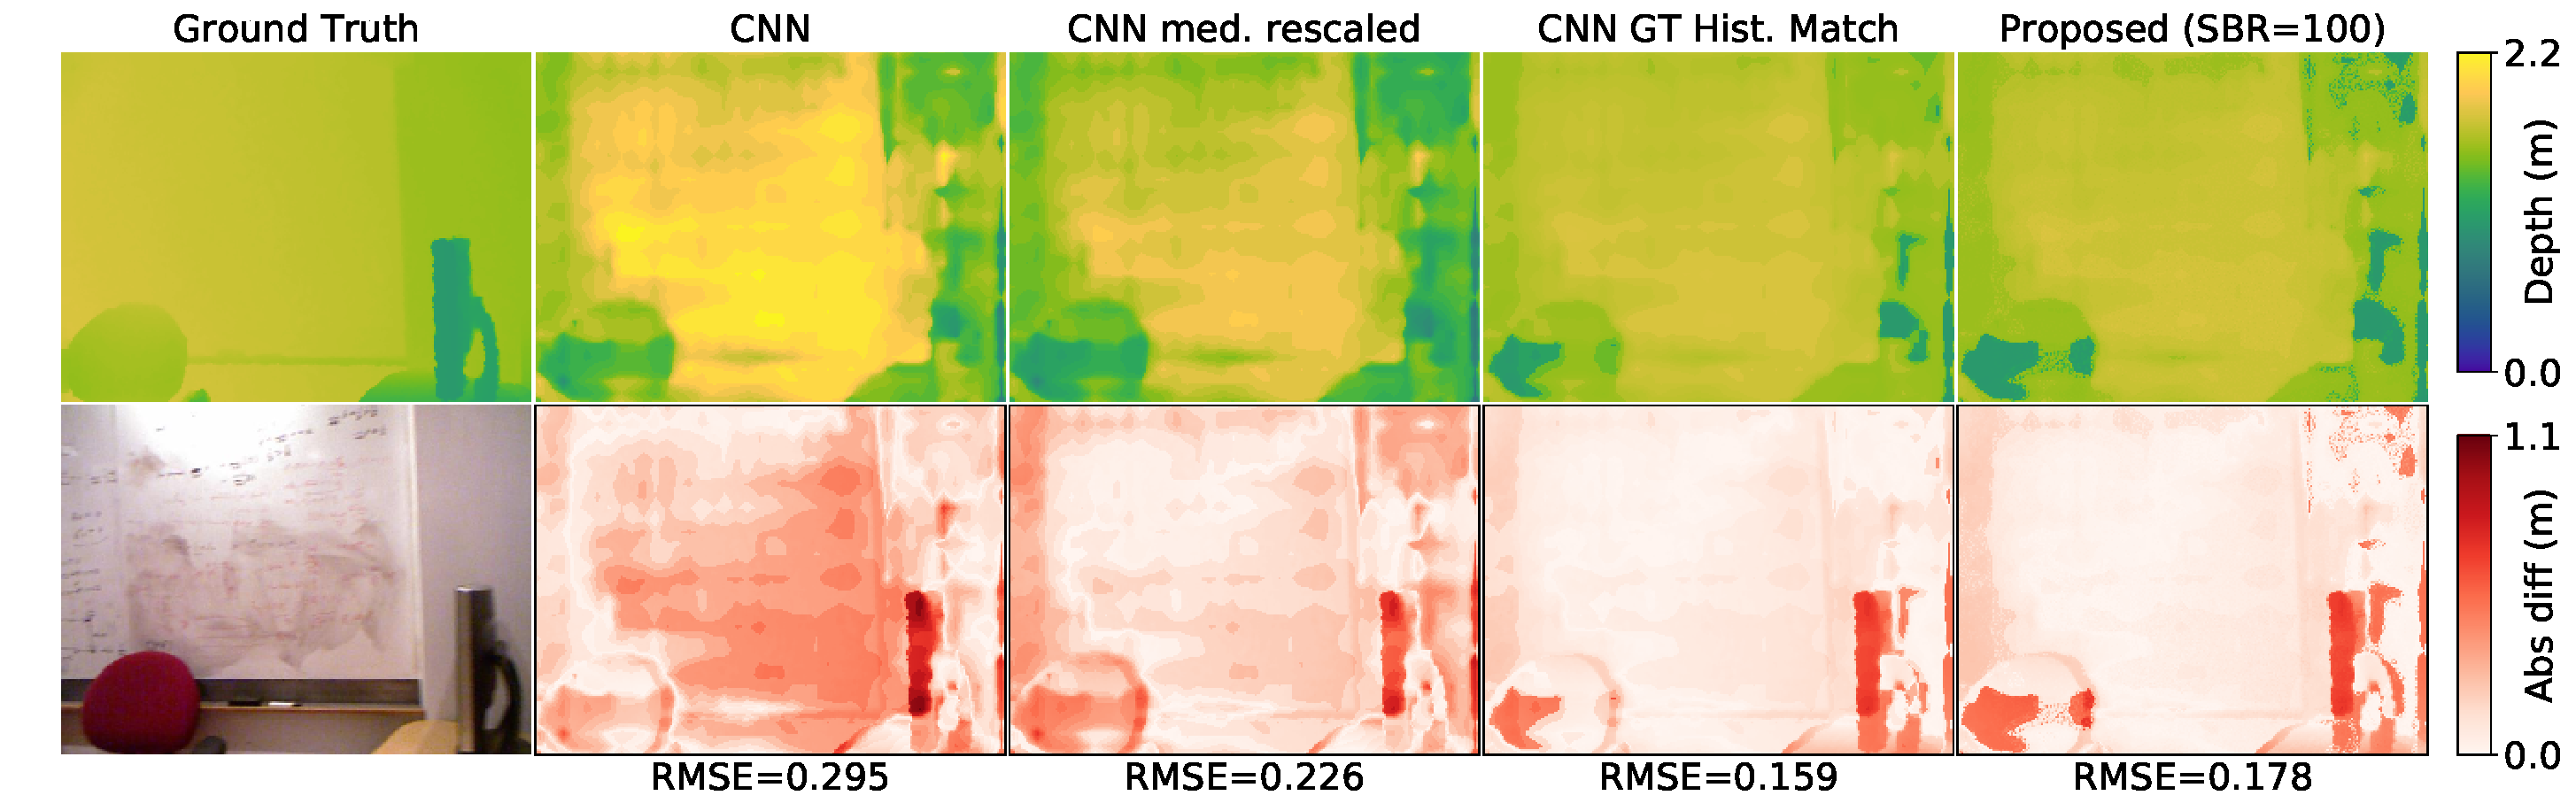
\includegraphics[width=\textwidth]{sections/figures/comparison/dorn_14_comparison.png}
  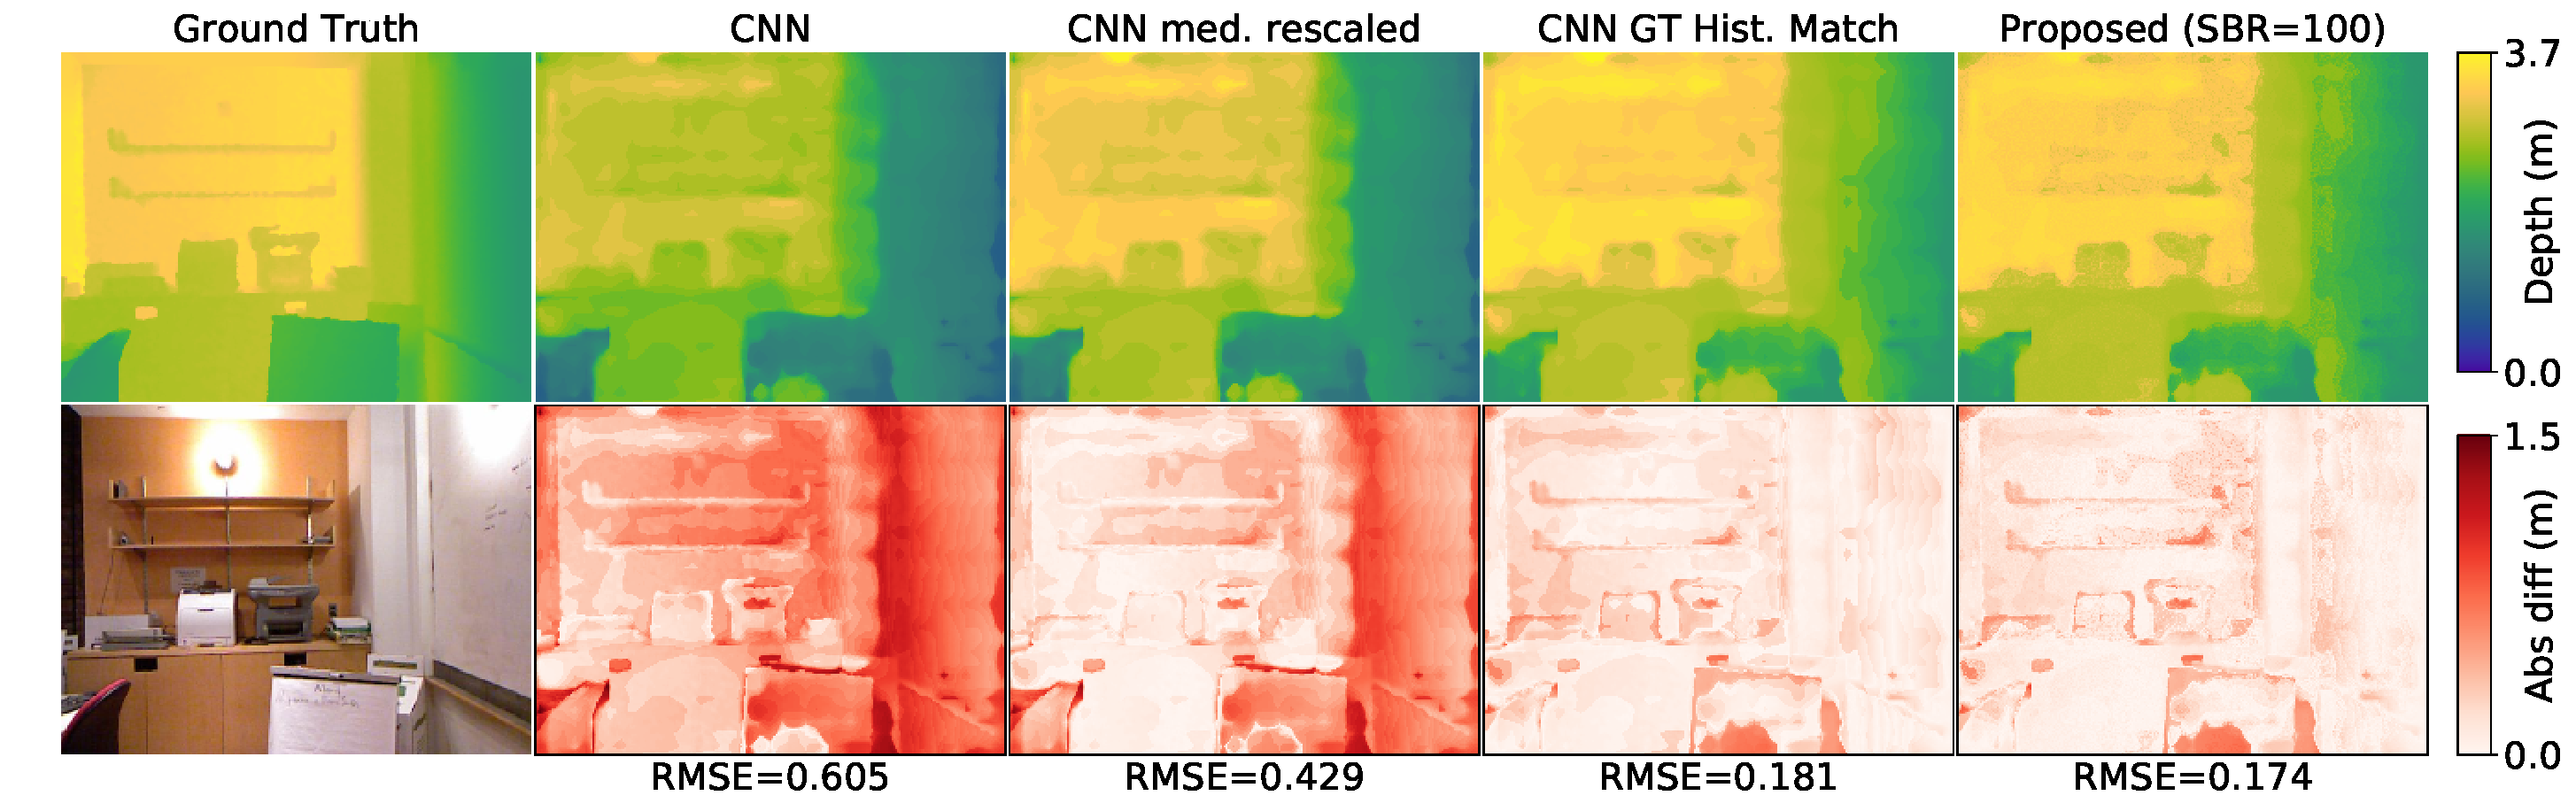
\includegraphics[width=\textwidth]{sections/figures/comparison/dorn_15_comparison.png}
  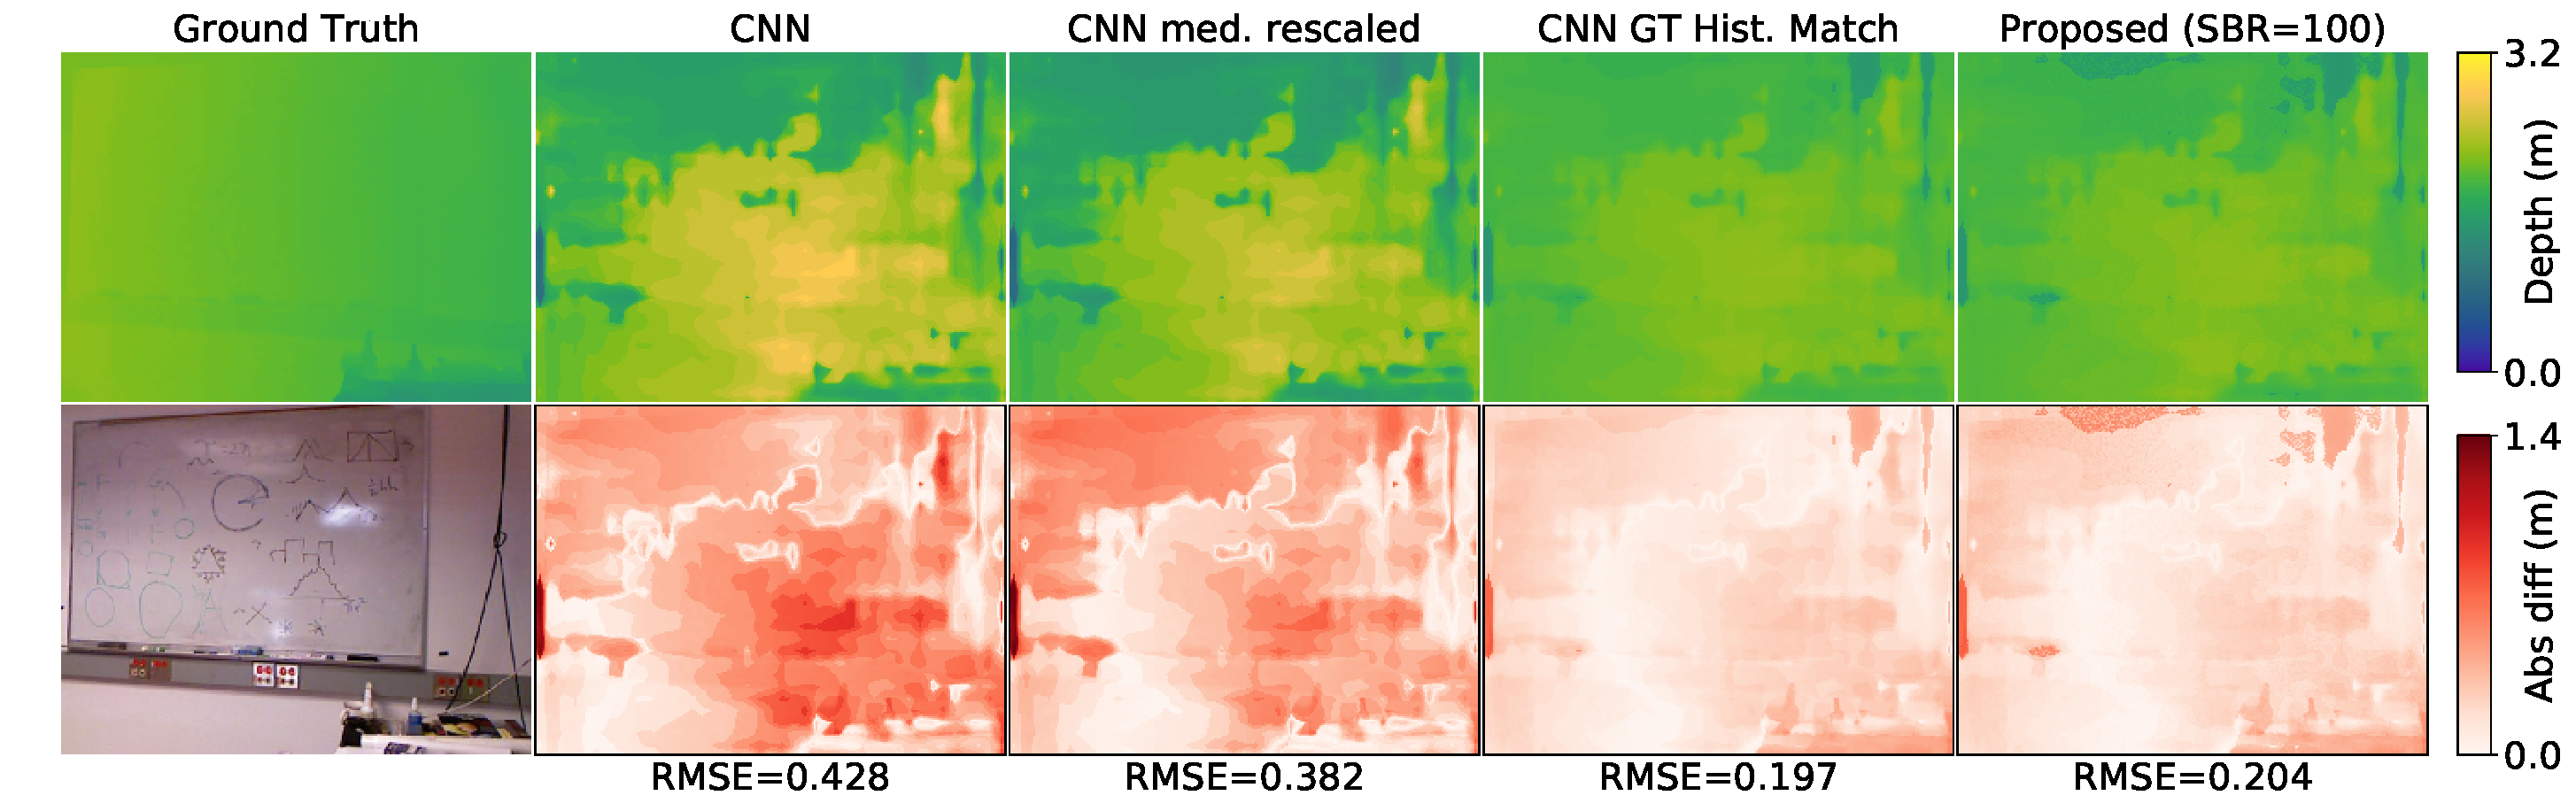
\includegraphics[width=\textwidth]{sections/figures/comparison/dorn_23_comparison.png}
  \caption{Results on DORN}
\end{figure*}
\begin{figure*}
  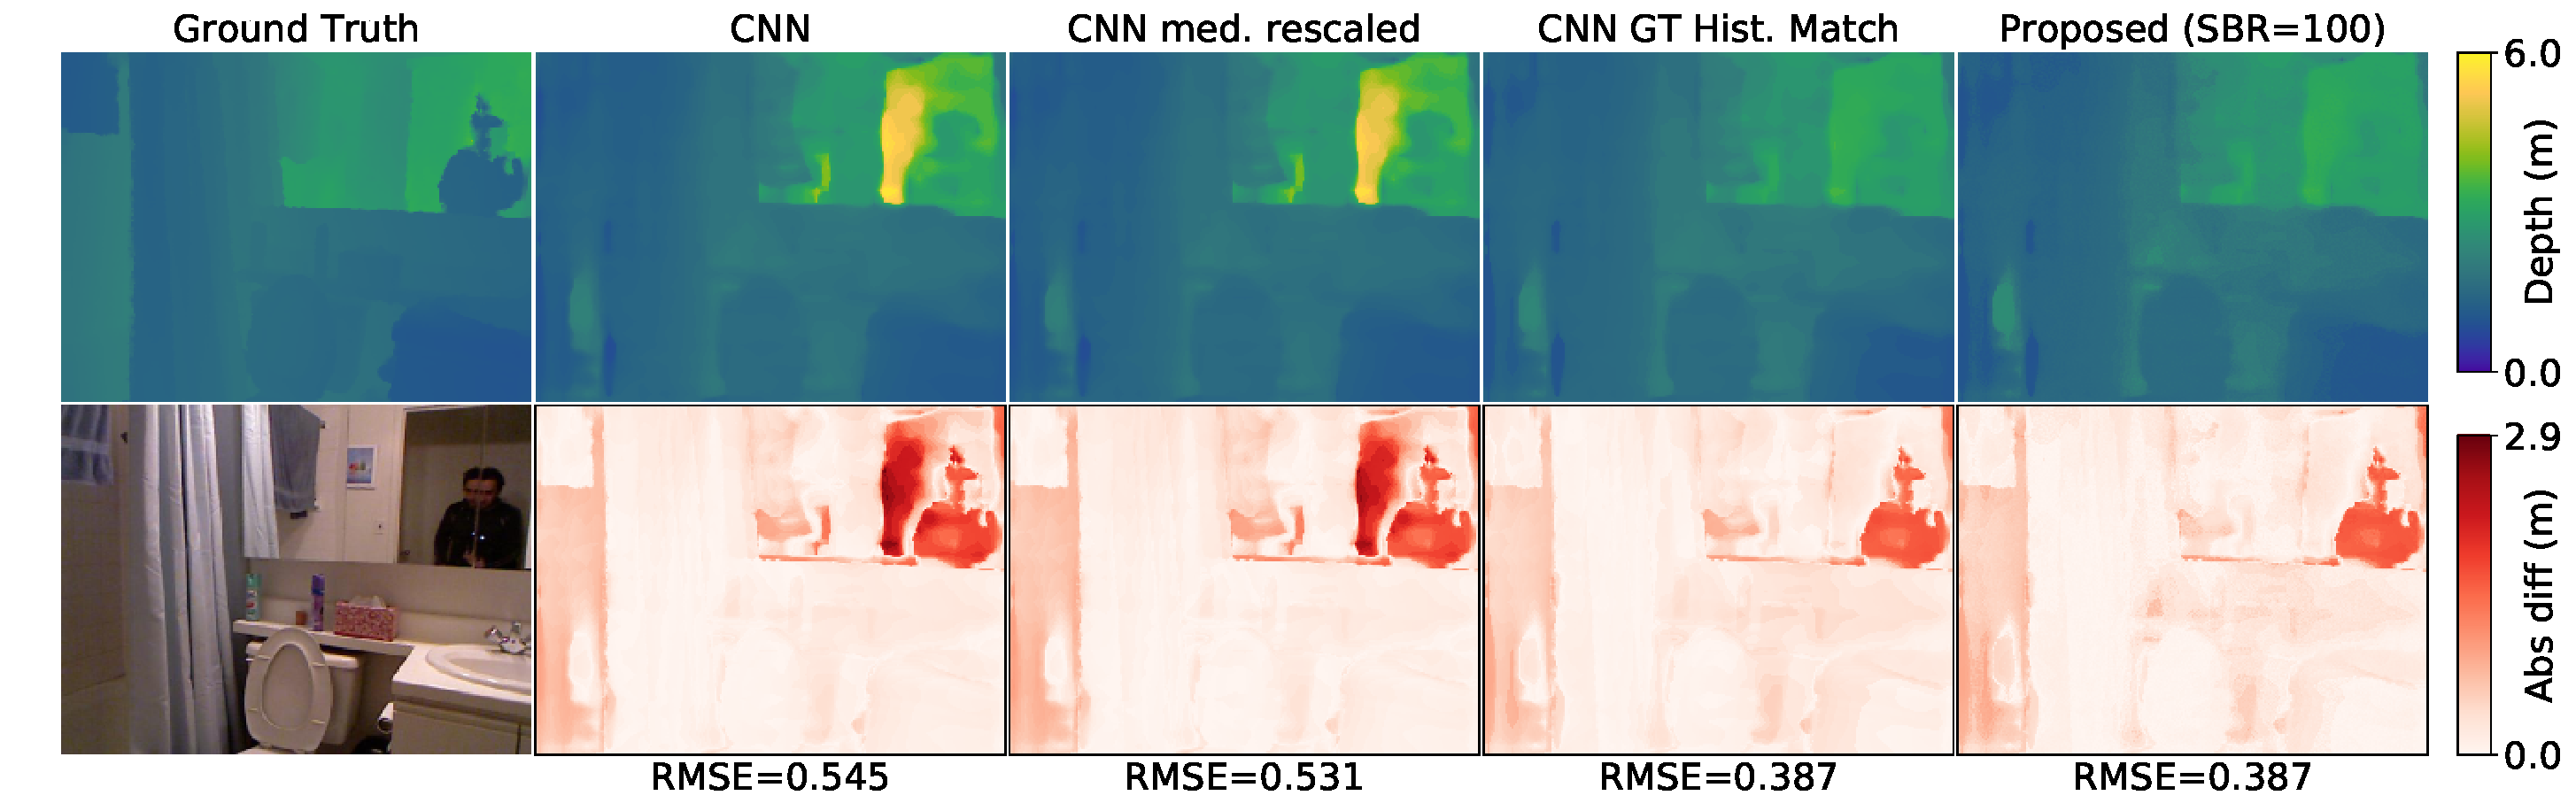
\includegraphics[width=\textwidth]{sections/figures/comparison/dorn_26_comparison.png}
  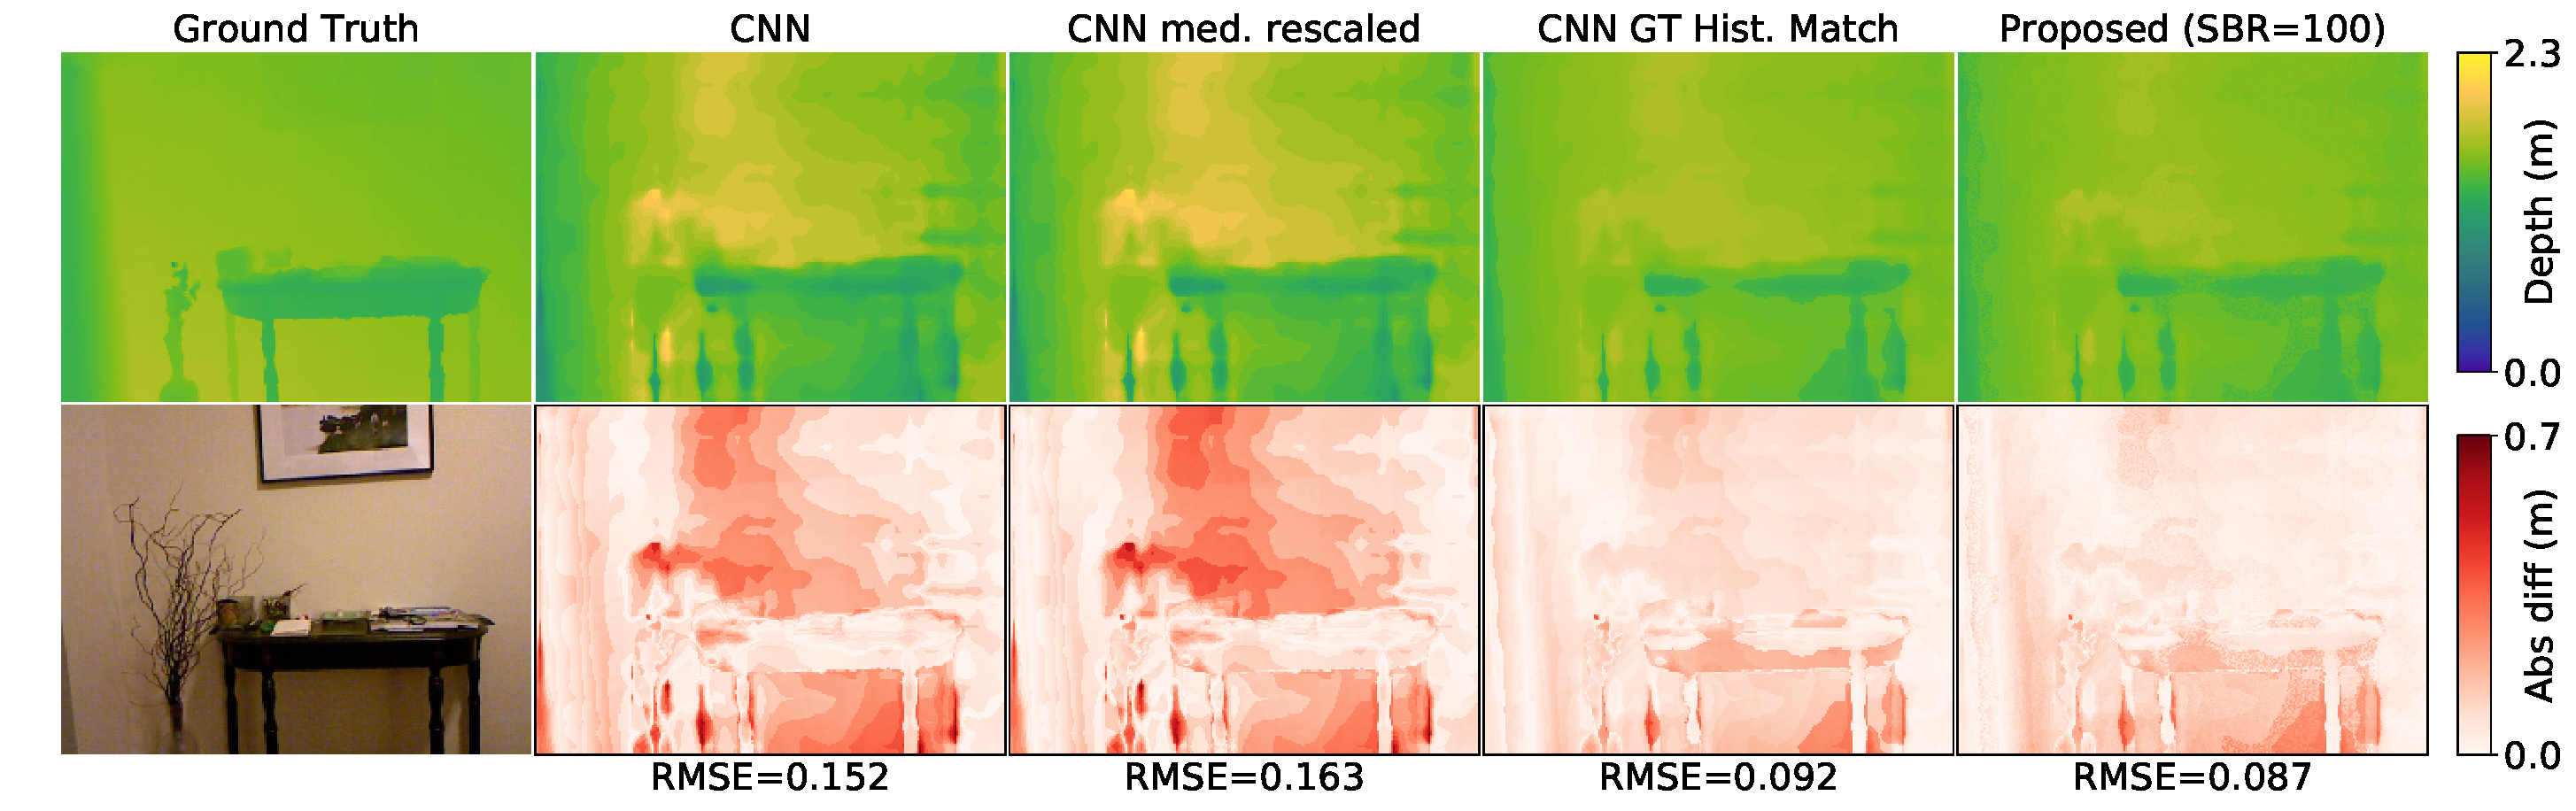
\includegraphics[width=\textwidth]{sections/figures/comparison/dorn_63_comparison.png}
  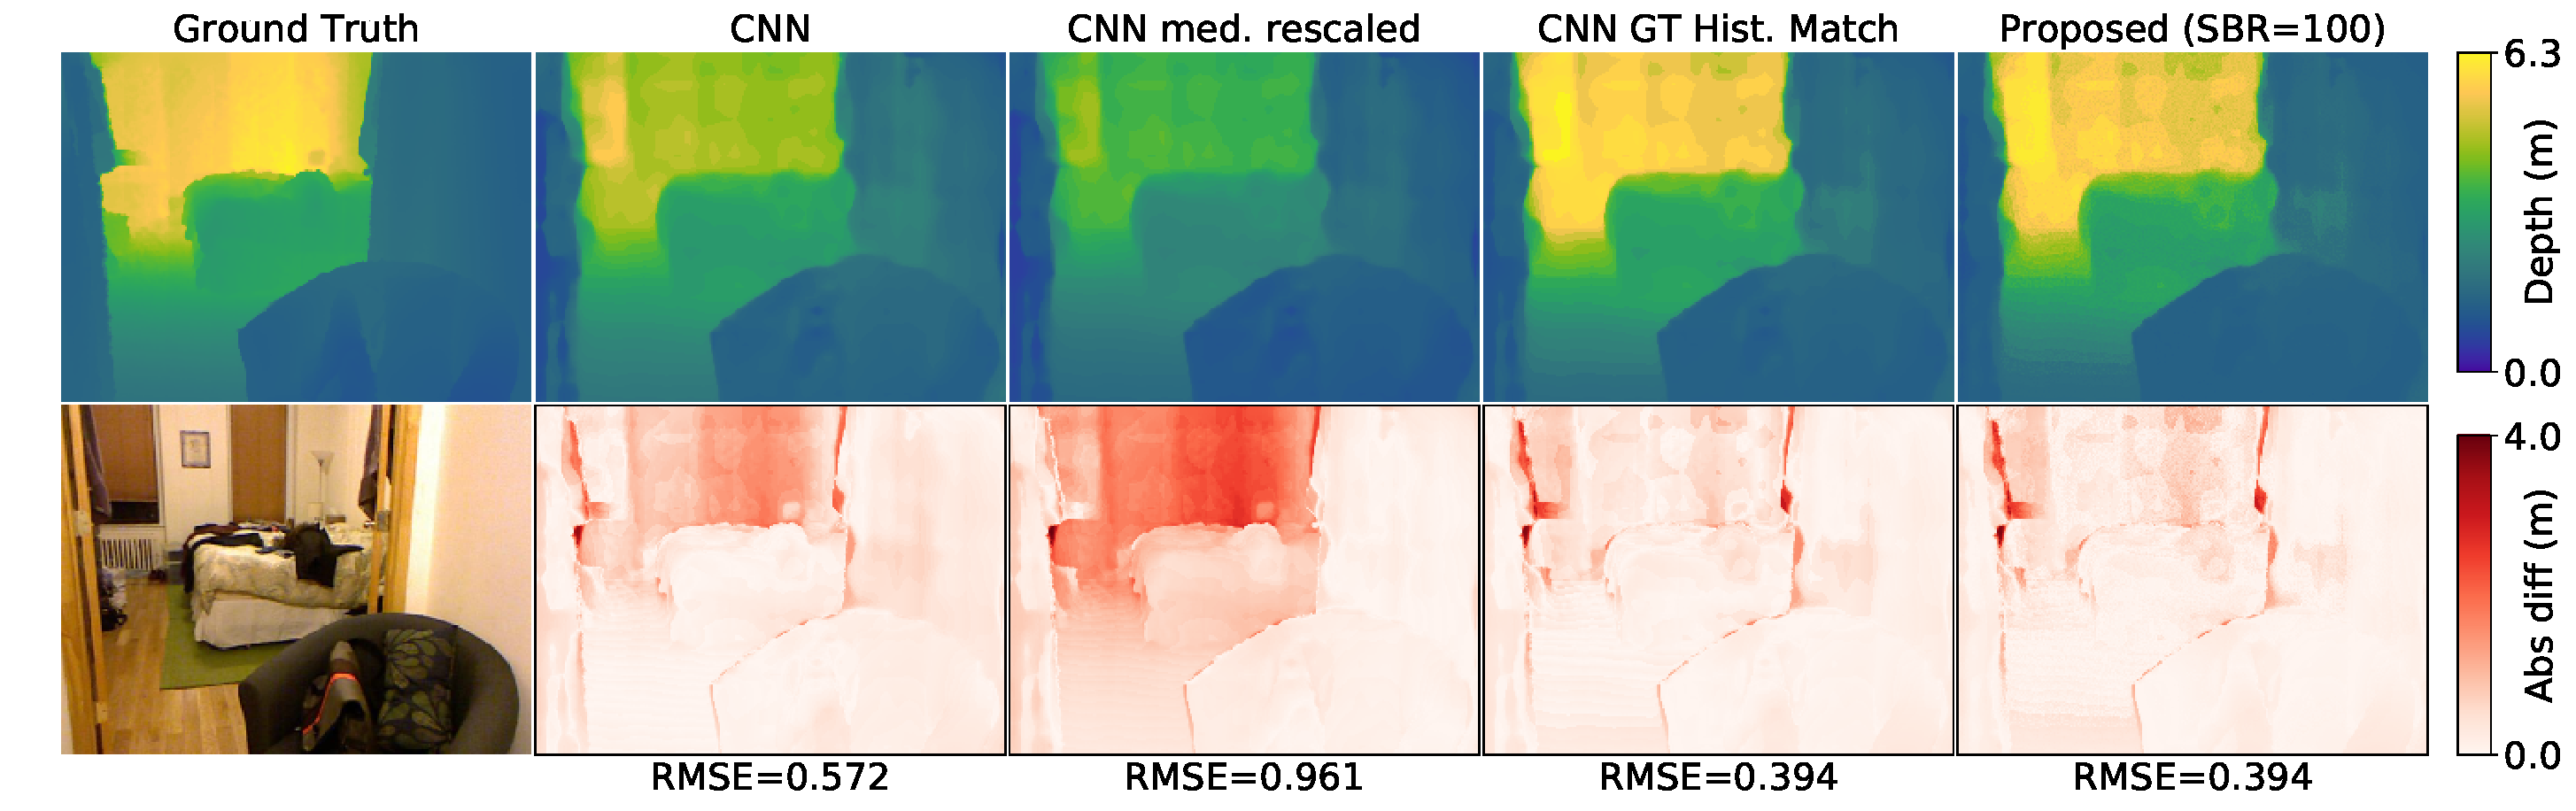
\includegraphics[width=\textwidth]{sections/figures/comparison/dorn_67_comparison.png}
  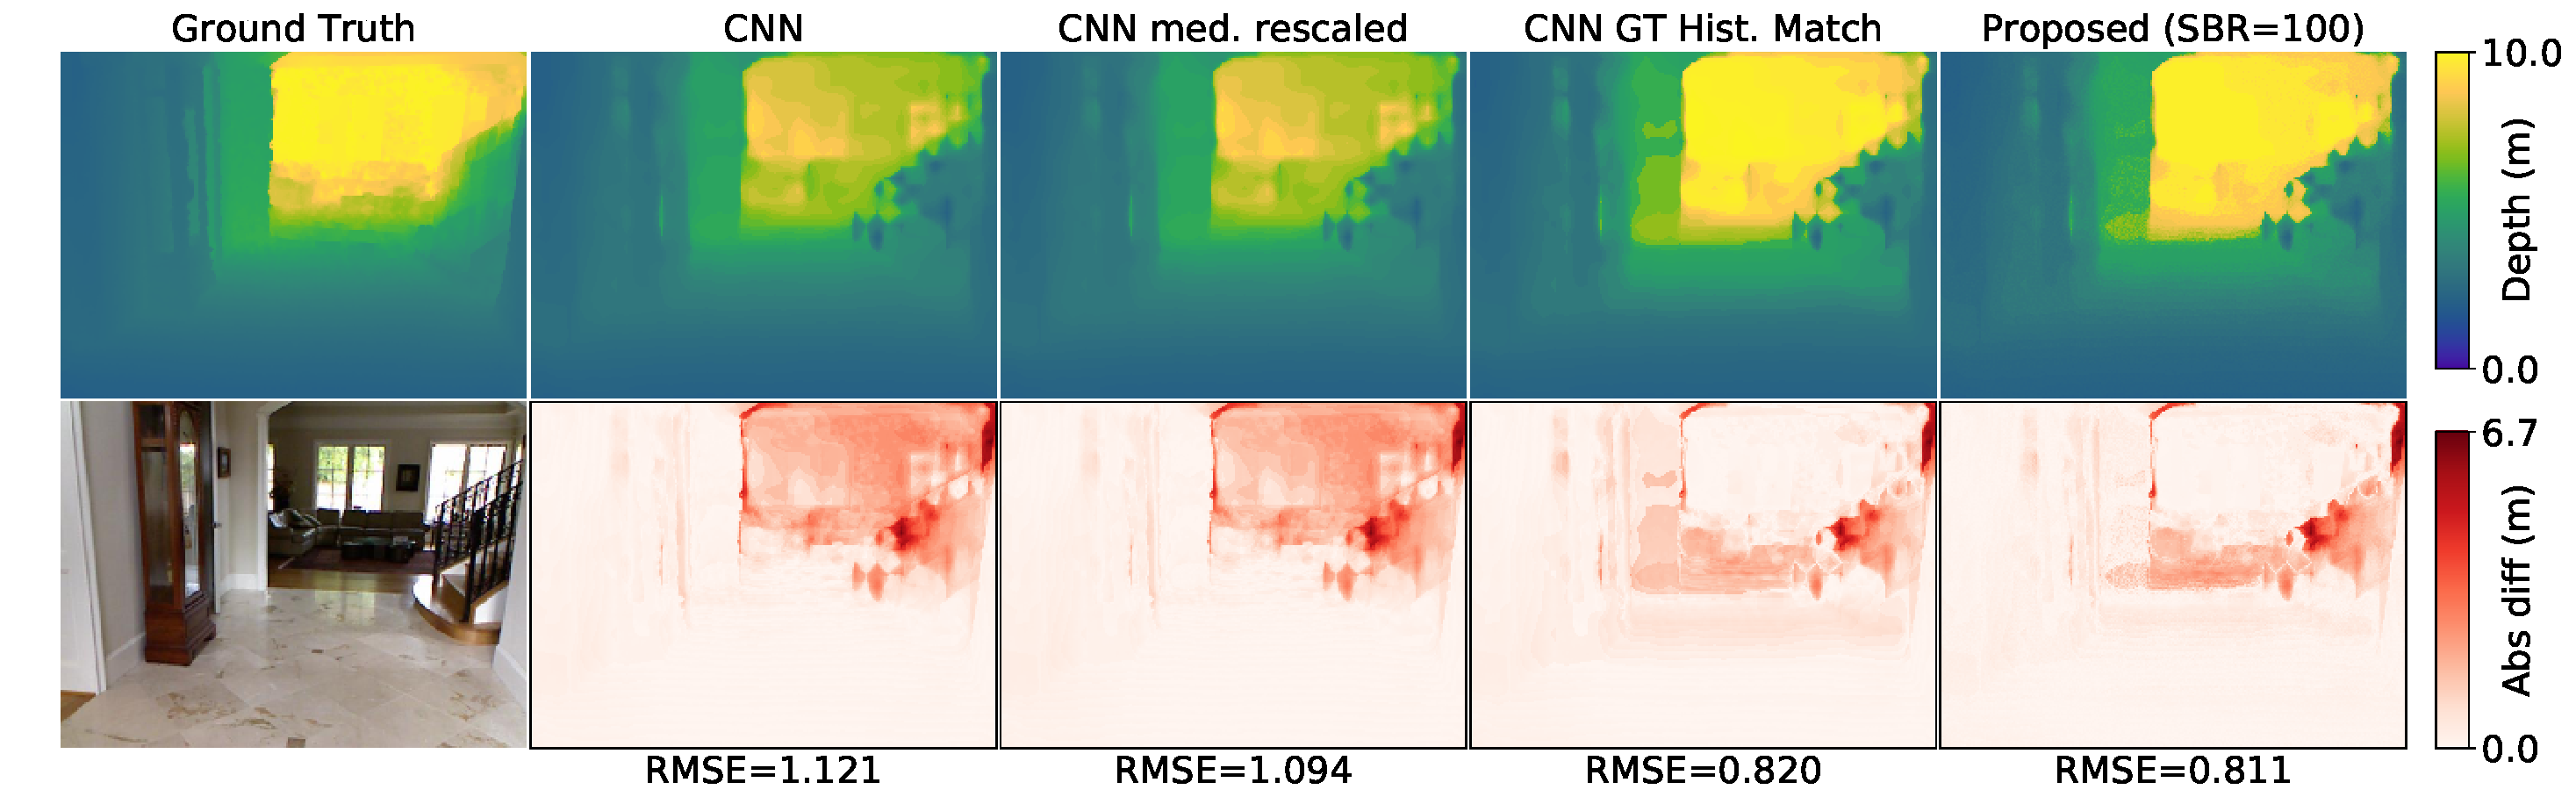
\includegraphics[width=\textwidth]{sections/figures/comparison/dorn_140_comparison.png}
  \caption{Results on DORN}
\end{figure*}
\begin{figure*}
  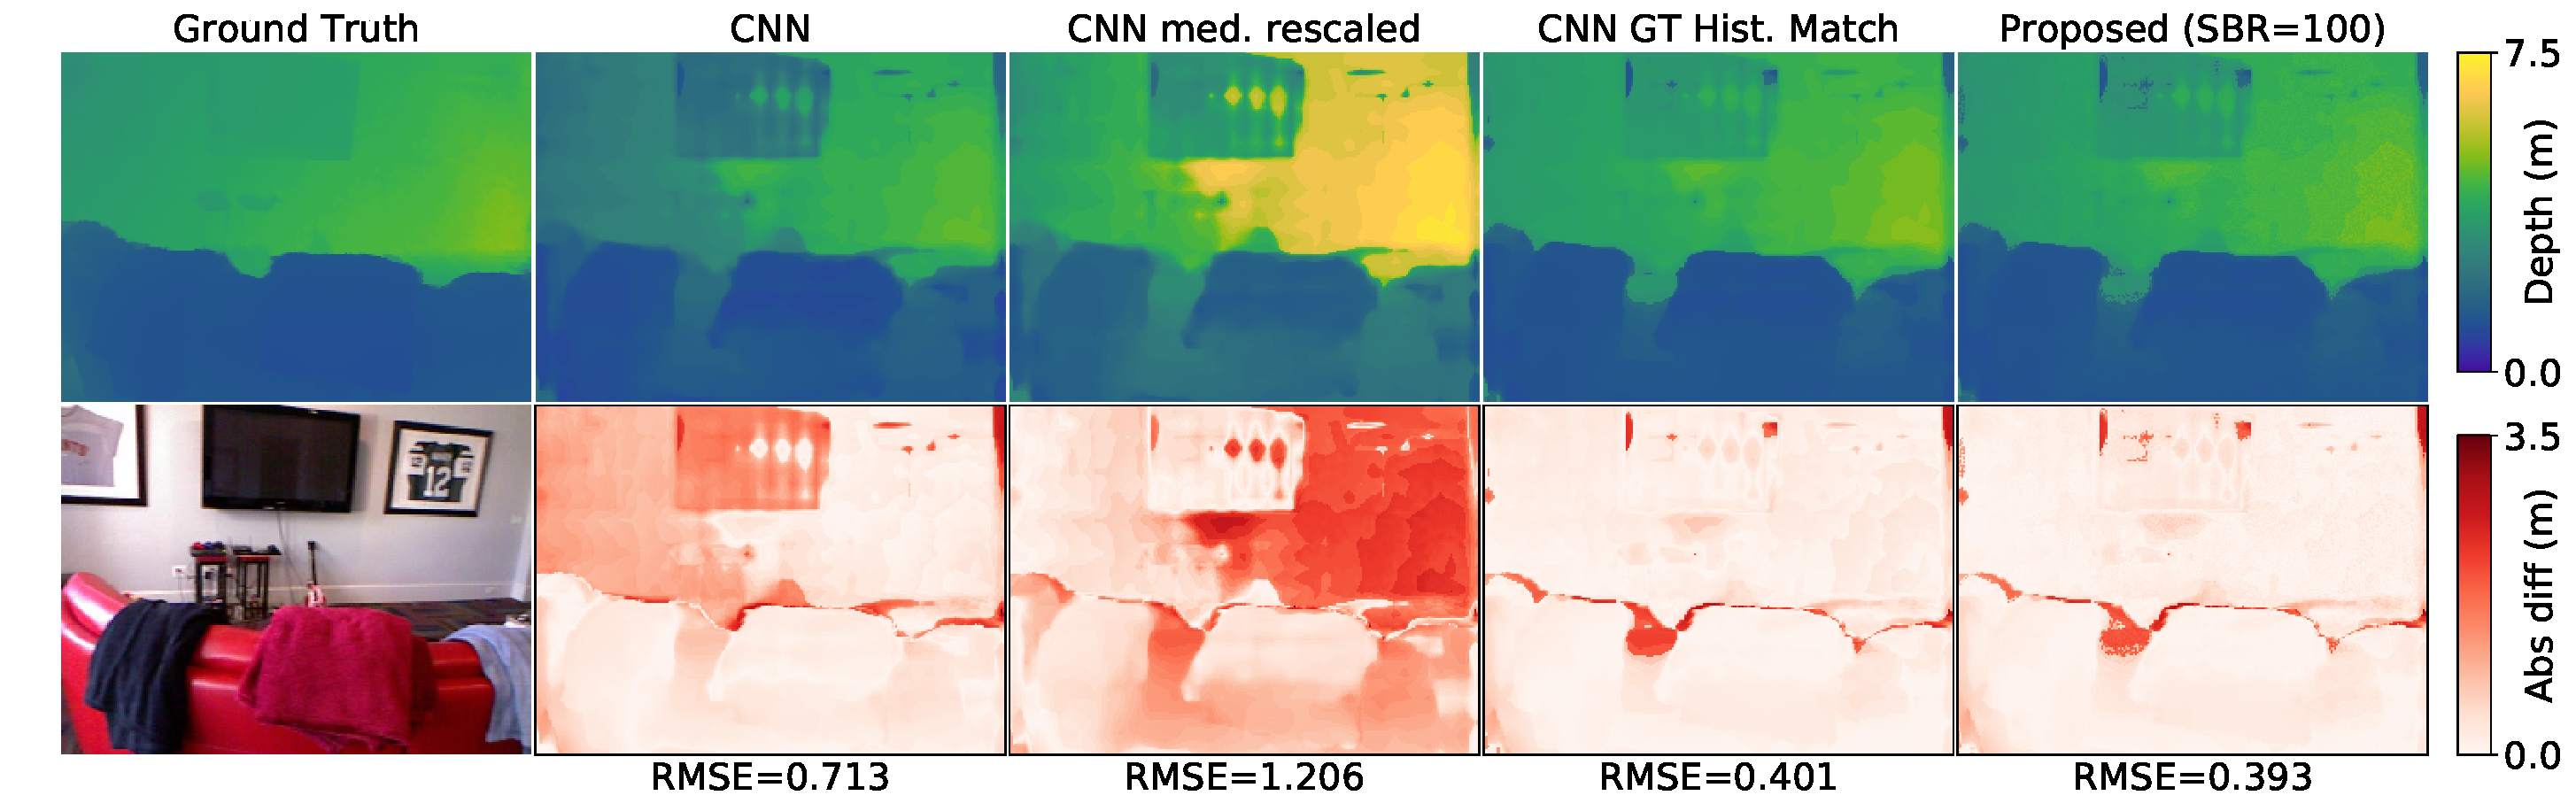
\includegraphics[width=\textwidth]{sections/figures/comparison/dorn_170_comparison.png}
  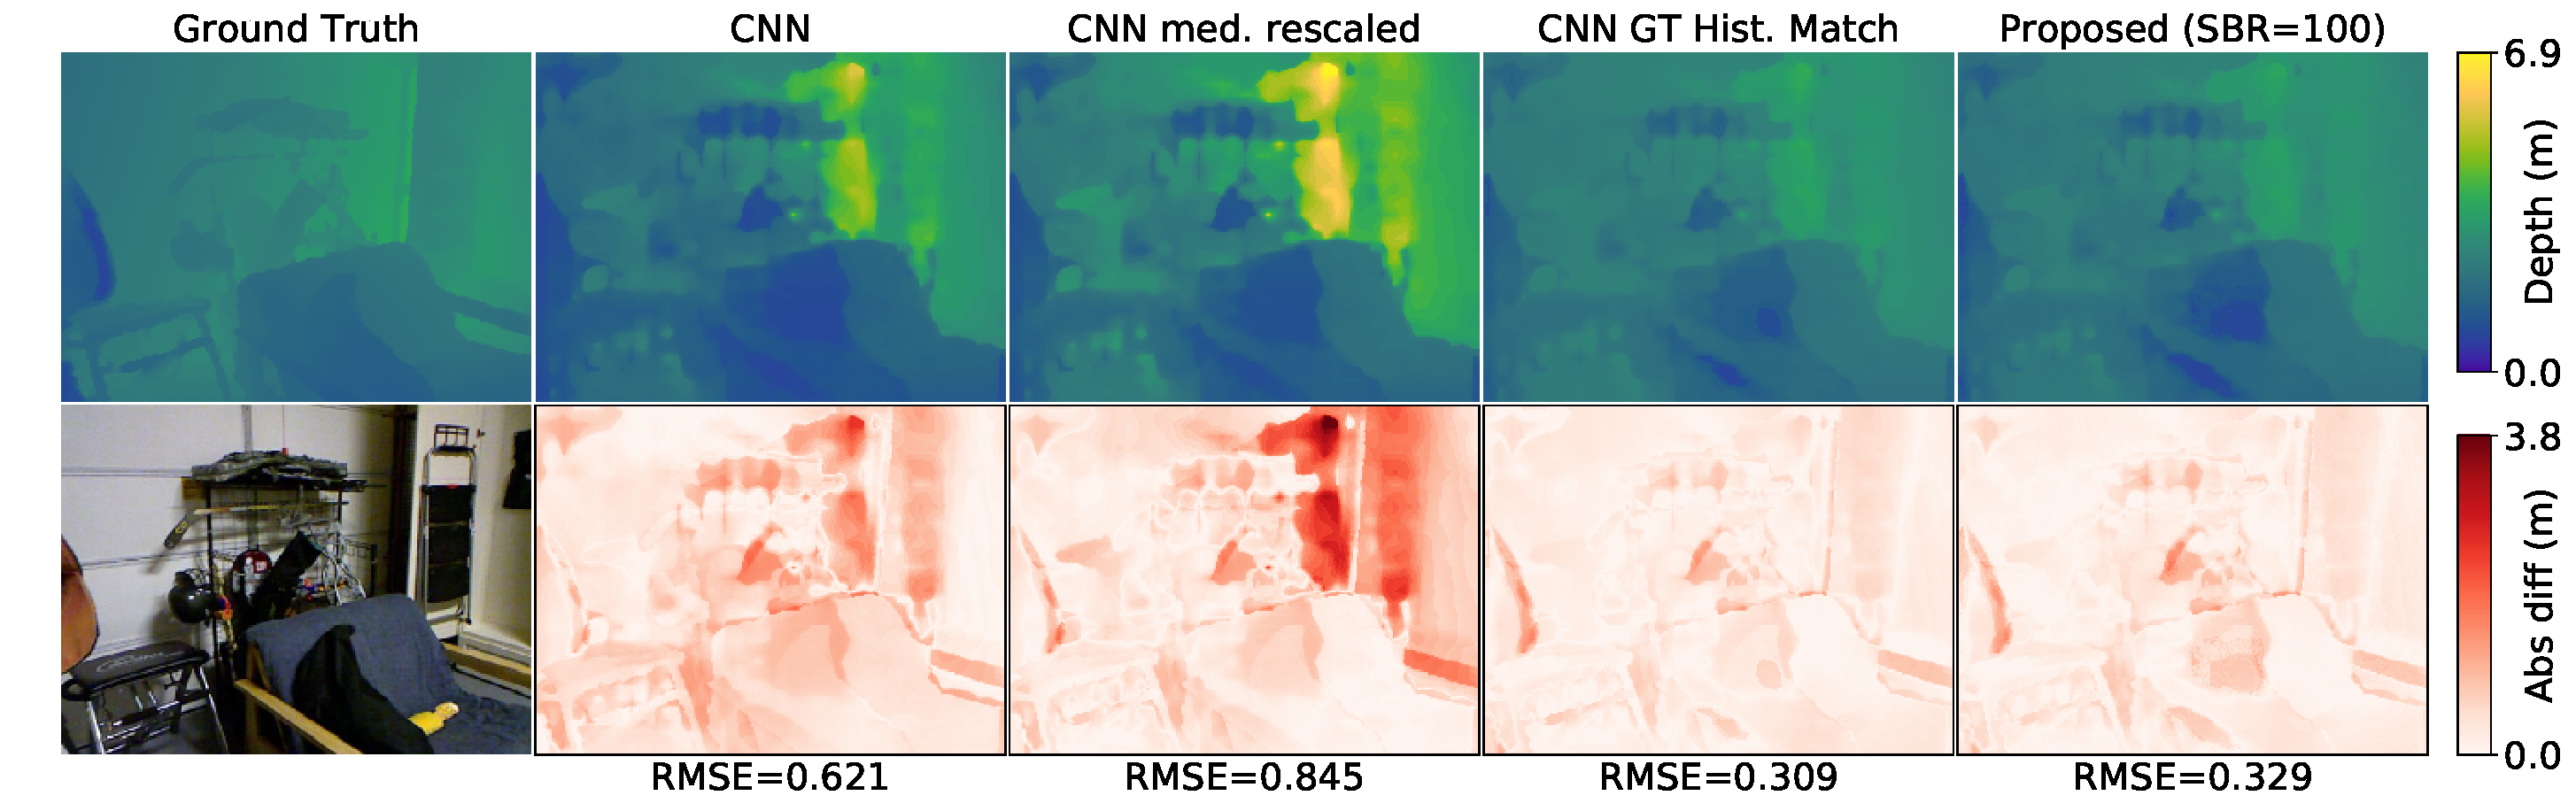
\includegraphics[width=\textwidth]{sections/figures/comparison/dorn_522_comparison.png}
  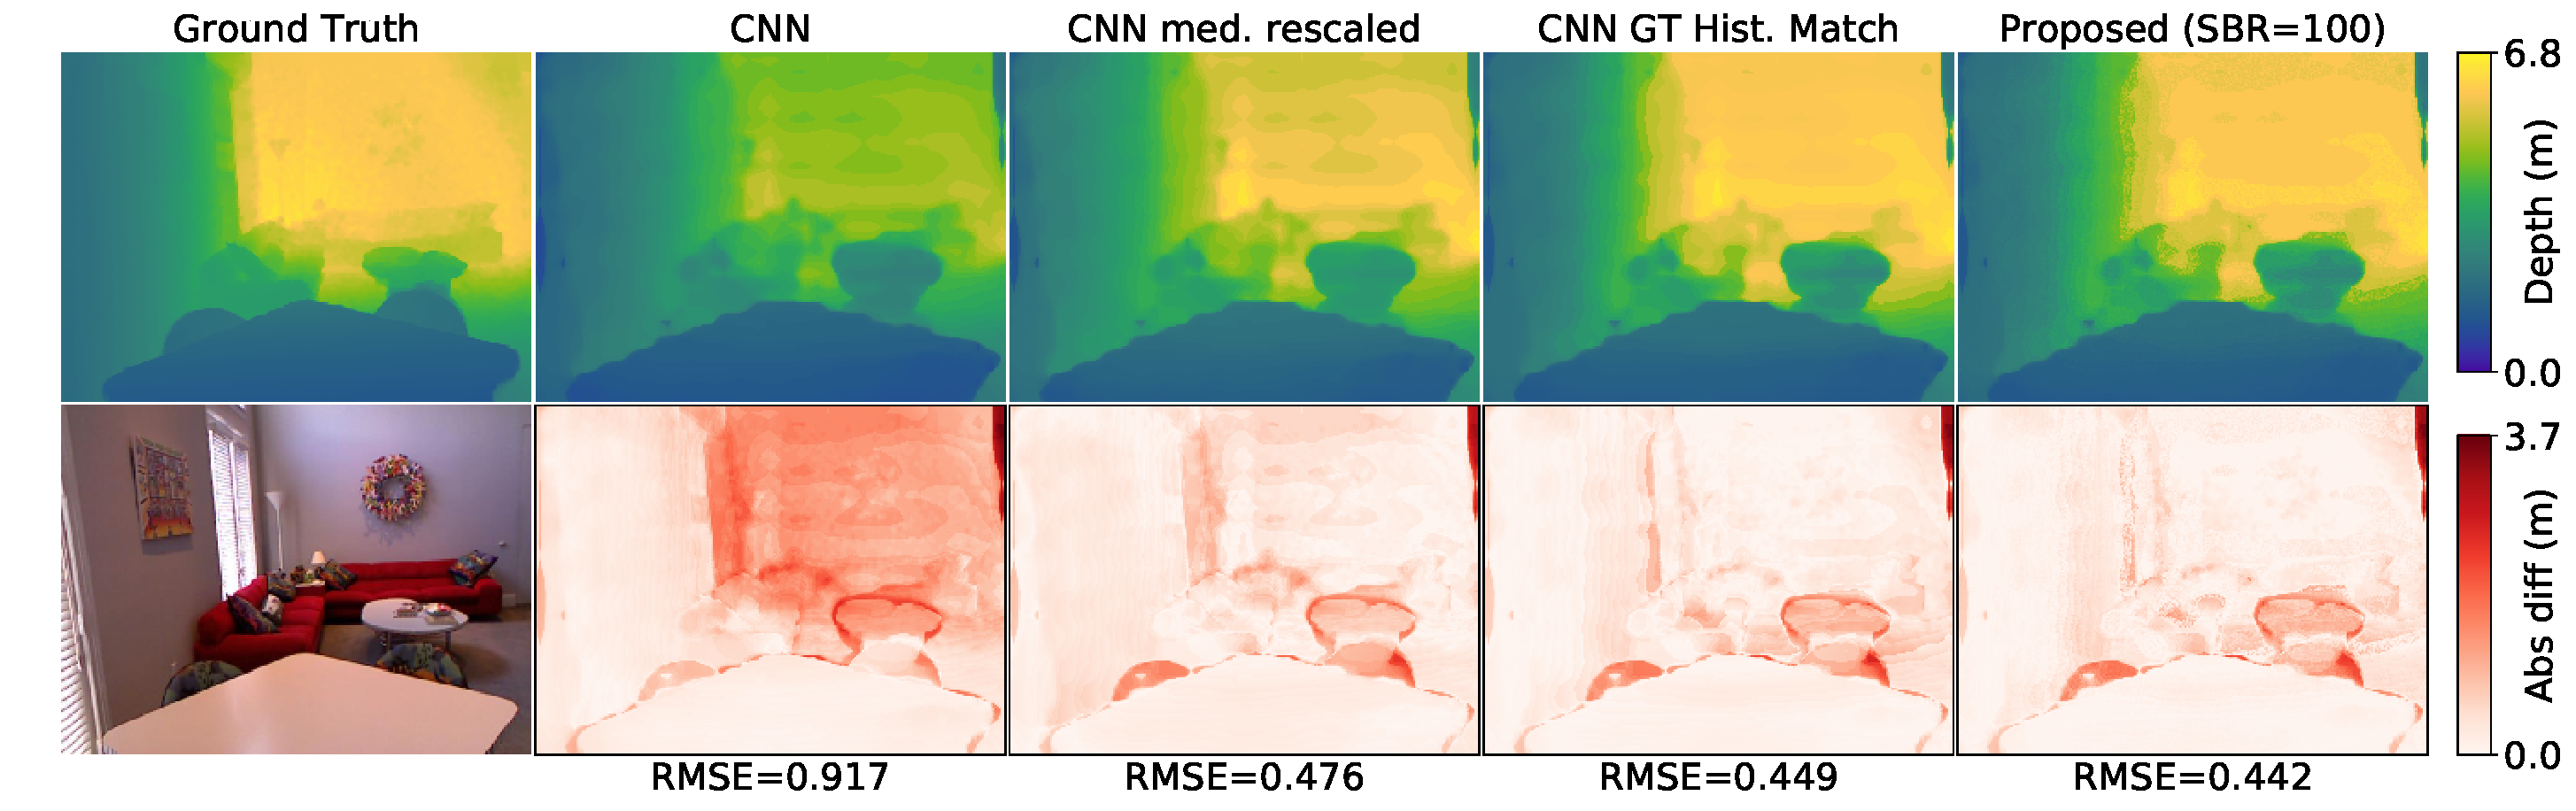
\includegraphics[width=\textwidth]{sections/figures/comparison/dorn_548_comparison.png}
  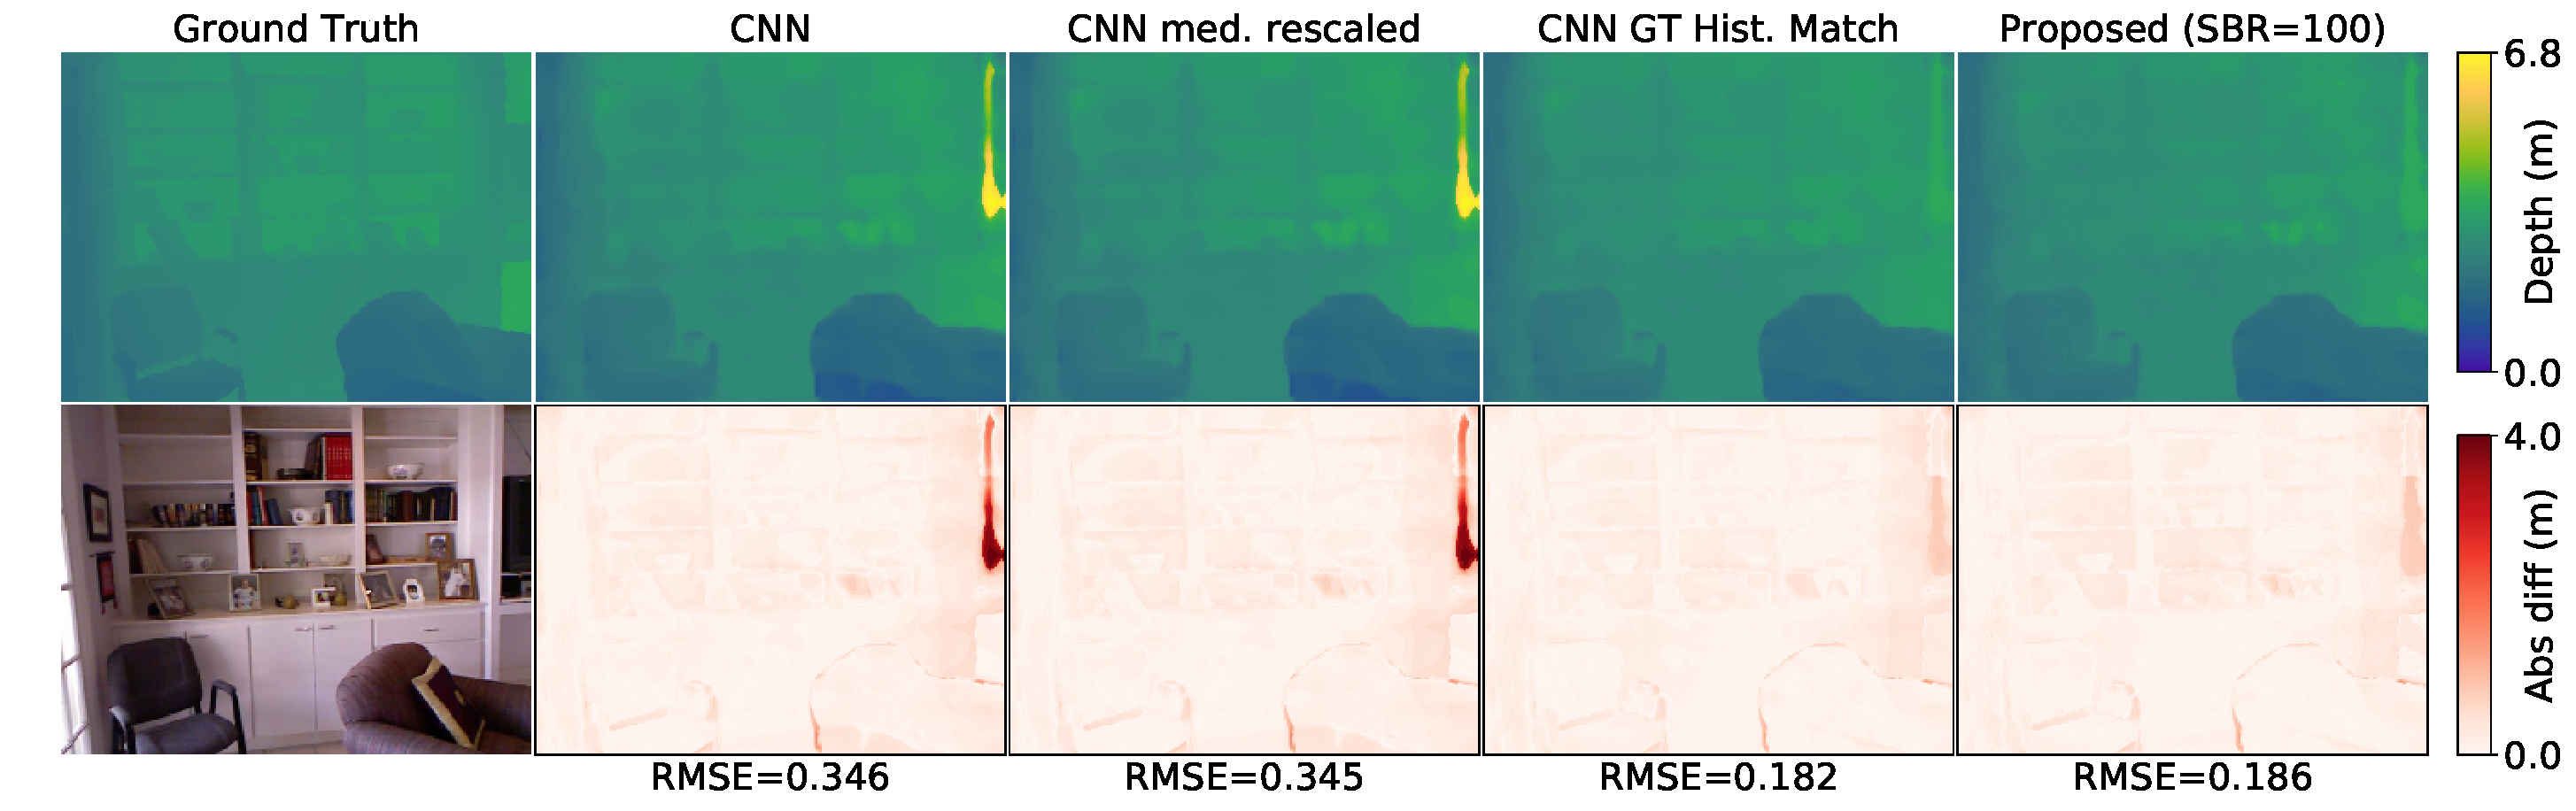
\includegraphics[width=\textwidth]{sections/figures/comparison/dorn_569_comparison.png}
  \caption{Results on DORN}
\end{figure*}
\begin{figure*}
  \includegraphics[width=\textwidth]{sections/figures/comparison/dorn_585_comparison.png}
  \includegraphics[width=\textwidth]{sections/figures/comparison/dorn_633_comparison.png}
  \includegraphics[width=\textwidth]{sections/figures/comparison/dorn_105_comparison.png}
  \includegraphics[width=\textwidth]{sections/figures/comparison/dorn_220_comparison.png}
  \caption{Results on DORN}
\end{figure*}
\begin{figure*}
  \includegraphics[width=\textwidth]{sections/figures/comparison/dorn_252_comparison.png}
  \includegraphics[width=\textwidth]{sections/figures/comparison/dorn_259_comparison.png}
  \includegraphics[width=\textwidth]{sections/figures/comparison/dorn_178_comparison.png}
  \includegraphics[width=\textwidth]{sections/figures/comparison/dorn_219_comparison.png}
  \caption{Results on DORN}
\end{figure*}
\begin{figure*}
  \includegraphics[width=\textwidth]{sections/figures/comparison/dorn_280_comparison.png}
  \includegraphics[width=\textwidth]{sections/figures/comparison/dorn_293_comparison.png}
  \includegraphics[width=\textwidth]{sections/figures/comparison/dorn_313_comparison.png}
  \includegraphics[width=\textwidth]{sections/figures/comparison/dorn_413_comparison.png}
  \caption{Results on DORN}
\end{figure*}
\begin{figure*}
  \includegraphics[width=\textwidth]{sections/figures/comparison/dorn_477_comparison.png}
  \includegraphics[width=\textwidth]{sections/figures/comparison/dorn_502_comparison.png}
%  \includegraphics[width=\textwidth]{sections/figures/comparison/dorn_428_comparison.png}
%  \includegraphics[width=\textwidth]{sections/figures/comparison/dorn_428_comparison.png}
  \caption{Results on DORN}
\end{figure*}
>>>>>>> ac23c73116b7fdd108ca4951a414a00ea9b25df3
% Densedepth:
% - Office: 18, 21
% - Bathroom: 25, 194, 285
% - Bookstore: 42
% - Kitchen: 52, 53, 103, 224, 226, 352, 362, 379
% - Office: 107, 187
% - Living Room: 140, 244, 527, 529
% - Dining Room: 219, 329, 346, 616
% - Bedroom: 390, 412, 420, 428, 457*, 468*, 477, 499
% Failure Cases: 258, 338(?), 341, 537 649 (minor)
% 
% DORN:
% - Office: 8, 14, 15, 23, 26
% - Living room: 63, 67, 140, 170, 522, 548, 569, 585, 633
% - Office: 105, 220, 252, 259* (interesting)
% - Kitchen: 178
% - Dining Room: 219
% - Bathroom: 280, 293, 313
% - Bedroom: 413, 477, 502
% 
% Failure Cases: 96, 266(?)
 

% \begin{figure}
%   \includegraphics[width=\textwidth/2]{sections/figures/comparison.jpeg}
%   \caption{\textbf{Comparing our results with other methods}}
% \end{figure}

  


